%! BibTeX Compiler = biber
\documentclass{article}
\usepackage{xcolor}
\definecolor{BLUELINK}{HTML}{0645AD}
\definecolor{DARKBLUELINK}{HTML}{0B0080}
\definecolor{LIGHTBLUELINK}{HTML}{3366BB}
\definecolor{PURPLELINK}{HTML}{663366}
\PassOptionsToPackage{hyphens}{url}
\usepackage[colorlinks=false ]{hyperref}
% for linking between references, figures, TOC, etc in the pdf document
\hypersetup{colorlinks,
linkcolor=DARKBLUELINK,
anchorcolor=DARKBLUELINK,
citecolor=DARKBLUELINK,
filecolor=DARKBLUELINK,
menucolor=DARKBLUELINK,
urlcolor=BLUELINK
} % Color citation links in purple
\PassOptionsToPackage{unicode}{hyperref}
\PassOptionsToPackage{naturalnames}{hyperref}

\usepackage[margin=60pt]{geometry}
\usepackage{amssymb,amsfonts,amsmath,amsthm,mathtools}
\usepackage{lmodern}
\usepackage{bm,bbold}
\usepackage{verbatim}
\usepackage{float}
\usepackage{listings, enumerate, enumitem}
\usepackage[export]{adjustbox}
\usepackage{tabu}
\usepackage{longtable}
\tabulinesep=0.6mm
\newcommand\cellwidth{\TX@col@width}
\usepackage{hhline}
\setlength{\arrayrulewidth}{1.2pt}
\usepackage{multicol,multirow,array}
\usepackage{etoolbox}
\AtBeginEnvironment{tabu}{\footnotesize}
\usepackage{booktabs}

\usepackage{graphicx}
\graphicspath{{artworks/}}
\makeatletter
\def\input@path{{artworks/}}
\makeatother
\pdfstringdefDisableCommands{%
\renewcommand*{\bm}[1]{#1}%
% any other necessary redefinitions
}
\newcommand{\specialcell}[2][c]{%
    \begin{tabular}[#1]{@{}c@{}}#2\end{tabular}}

\usepackage{xfrac, nicefrac}
\usepackage[backend=biber,style=nature]{biblatex}
\addbibresource{codon_models.bib}
\pdfinclusioncopyfonts=1

\begin{document}
\part*{Supplementary materials}
\tableofcontents
 
\pagebreak

\section{Rate of adaptation enrichment}
\subsection{Method summary}

\begin{center}
    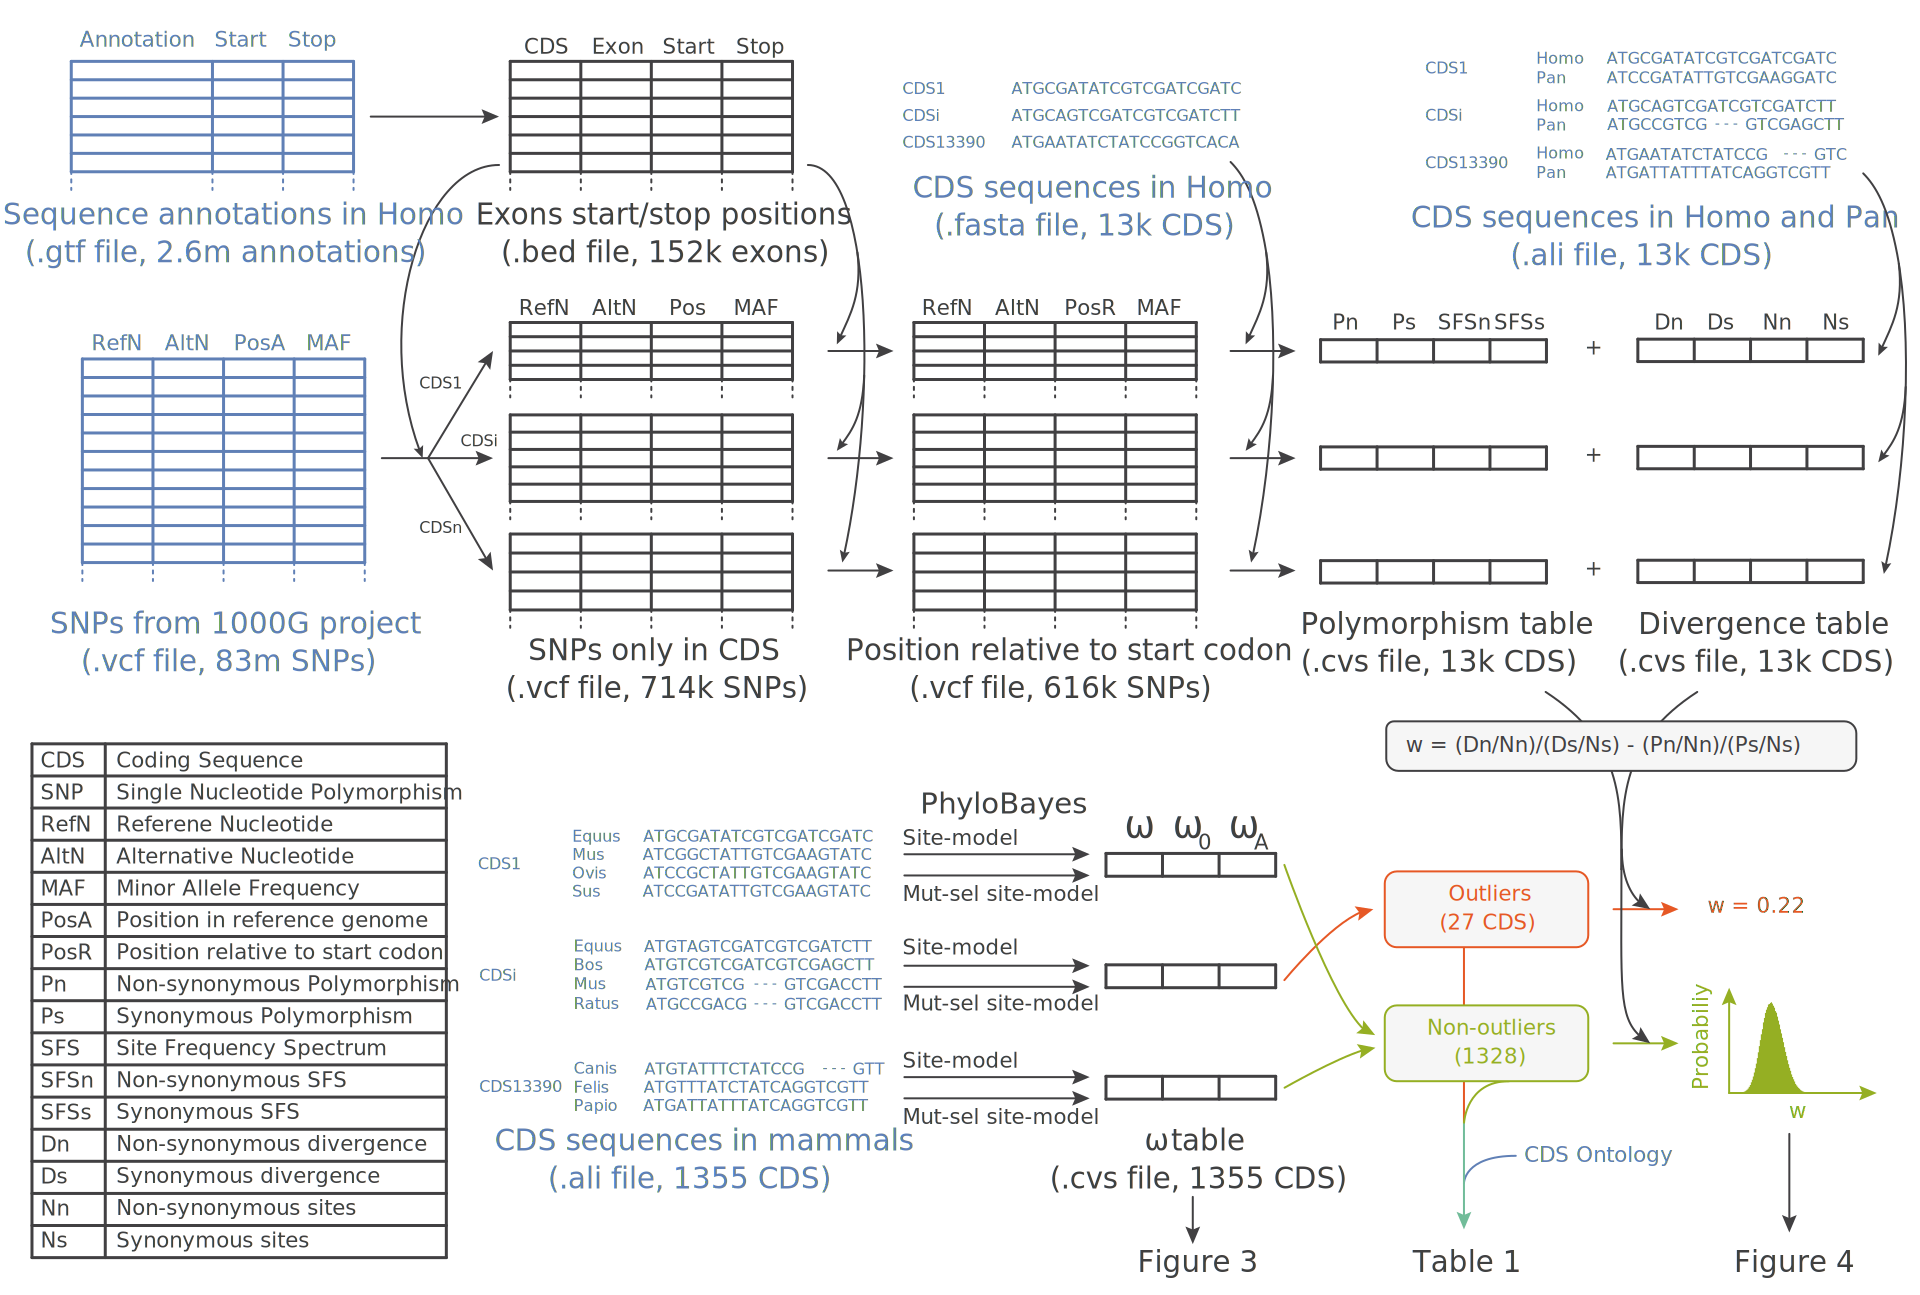
\includegraphics[width=\linewidth]{pipeline}
\end{center}

\subsection{Comparison - MK/PolyDFE/grapes}

\begin{center}
    \includegraphics[width=\linewidth]{results.pval}
    \includegraphics[width=\linewidth]{results.delta_wa} \\
    $\Delta \omega_{\text{A}} = \omega_{\text{A}}^{\text{Adaptive set}} - \omega_{\text{A}}^{\text{Nearly-neutral set}}$
\end{center}

\subsection{Mutation-selection codon model at gene level ($\bm{\alpha=0.005}$)}
\begin{center}
    \includegraphics[width=\linewidth]{no_control/gene-MutSel-0.0025-unfolded-MK-wA.pdf}
    \begin{adjustbox}{width = 1\textwidth}
        \begin{tabular}{|l|l|r|r|r|r|r|r|r|}
            \toprule
            Population & Species & \specialcell{$\omega_{\mathrm{A}}$ \\ Adaptive}                & \specialcell{$\left< \omega_{\mathrm{A}} \right>$ \\ Nearly-neutral}                & $\Delta \omega_{\mathrm{A}} $    & $p_{\mathrm{v}}$ & $p_{\mathrm{v}}^{\mathrm{adj}}$ & $\frac{\Delta\omega_{\mathrm{A}}}{\Delta\omega_{\mathrm{A}}^{\mathrm{phy}}}$ & $\pi_{\textrm{S}}$    \\
            \midrule
            Diverse (Equus)                    & Equus caballus          & $ 0.101$ & $-0.024$ & $ 0.125$ & $0.0$ & $\bm{0.0{^*}}$ & $ 1.029$ & $ 0.002$ \\
            Diverse (Canis)                  & Canis familiaris          & $ 0.084$ & $-0.006$ & $ 0.090$ & $0.0$ & $\bm{0.0{^*}}$ & $ 0.722$ & $ 0.004$ \\
            Iran (IRBT)               & Bos taurus        & $ 0.105$ & $ 0.058$ & $ 0.046$ & $ 0.002$    & $\bm{ 0.014{^*}}$    & $ 0.381$ & $ 0.008$ \\
            Uganda (UGBT)                  & Bos taurus        & $ 0.105$ & $ 0.059$ & $ 0.046$ & $ 0.001$ & $\bm{ 0.010{^*}}$ & $ 0.382$ & $ 0.008$ \\
            Australia (AUCH)                    & Capra hircus      & $ 0.088$ & $ 0.013$ & $ 0.075$ & $0.0$    & $\bm{0.0{^*}}$    & $ 0.611$ & $ 0.003$ \\
            France (FRCH)                    & Capra hircus        & $ 0.082$ & $ 0.012$ & $ 0.070$ & $ 0.001$    & $\bm{ 0.010{^*}}$    & $ 0.573$ & $ 0.003$ \\
            Iran (IRCA)                   & Capra aegagrus        & $ 0.103$ & $ 0.031$ & $ 0.073$ & $0.0$    & $\bm{0.0{^*}}$    & $ 0.593$ & $ 0.004$ \\
            Iran (IRCH)                 & Capra hircus        & $ 0.102$ & $ 0.020$ & $ 0.081$ & $0.0$    & $\bm{0.0{^*}}$    & $ 0.662$ & $ 0.004$ \\
            Italy (ITCH)                    & Capra hircus          & $ 0.080$ & $ 0.010$ & $ 0.070$ & $0.0$    & $\bm{0.0{^*}}$    & $ 0.571$ & $ 0.003$ \\
            Morocco (MOCH)                    & Capra hircus     & $ 0.078$ & $ 0.016$ & $ 0.062$ & $0.0$    & $\bm{0.0{^*}}$    & $ 0.504$ & $ 0.004$ \\
            Iran (IROA)                    & Ovis aries         & $ 0.172$ & $ 0.059$ & $ 0.113$ & $0.0$    & $\bm{0.0{^*}}$    & $ 0.919$ & $ 0.007$ \\
            Iran (IROO)                 & Ovis orientalis          & $ 0.166$ & $ 0.062$ & $ 0.104$ & $0.0$    & $\bm{0.0{^*}}$    & $ 0.841$ & $ 0.009$ \\
            Iran (IROV)                 & Ovis vignei          & $ 0.169$ & $ 0.079$ & $ 0.090$ & $0.0$    & $\bm{0.0{^*}}$    & $ 0.726$ & $ 0.005$ \\
            Various (ISGC)                       & Ovis aries & $ 0.167$ & $ 0.062$ & $ 0.105$ & $0.0$    & $\bm{0.0{^*}}$    & $ 0.847$ & $ 0.008$ \\
            Morocco (MOOA) & Ovis aries & $ 0.174$ & $ 0.060$ & $ 0.113$ & $0.0$ & $\bm{0.0{^*}}$ & $ 0.916$ & $ 0.008$ \\
            Barbados                       & Chlorocebus sabaeus & $ 0.096$ & $ 0.003$ & $ 0.093$ & $0.0$    & $\bm{0.0{^*}}$    & $ 0.755$ & $ 0.003$ \\
            Central African Republic (CAR)                         & Chlorocebus sabaeus & $ 0.076$ & $ 0.020$ & $ 0.056$ & $0.0$    & $\bm{0.0{^*}}$    & $ 0.451$ & $ 0.006$ \\
            Ethiopia                          & Chlorocebus sabaeus & $ 0.051$ & $-0.011$ & $ 0.062$ & $0.0$    & $\bm{0.0{^*}}$    & $ 0.504$ & $ 0.005$ \\
            Gambia                          & Chlorocebus sabaeus & $ 0.062$ & $ 0.010$ & $ 0.052$ & $0.0$ & $\bm{0.0{^*}}$        & $ 0.423$ & $ 0.005$ \\
            Kenya              & Chlorocebus sabaeus & $ 0.079$ & $ 0.018$ & $ 0.061$ & $0.0$    & $\bm{0.0{^*}}$ & $ 0.497$ & $ 0.004$ \\
            Nevis               & Chlorocebus sabaeus & $ 0.045$ & $ 0.006$ & $ 0.039$ & $ 0.014$ & $ 0.070~~$ & $ 0.319$ & $ 0.003$ \\
            South Africa (SA)                         & Chlorocebus sabaeus & $ 0.075$ & $ 0.002$ & $ 0.072$ & $0.0$    & $\bm{0.0{^*}}$    & $ 0.587$ & $ 0.006$ \\
            Saint Kitts (SK)                  & Chlorocebus sabaeus        & $ 0.049$ & $ 0.001$ & $ 0.047$ & $ 0.002$ & $\bm{ 0.014{^*}}$        & $ 0.384$ & $ 0.004$ \\
            Zambia        & Chlorocebus sabaeus        & $ 0.077$ & $ 0.004$ & $ 0.073$ & $0.0$ & $\bm{0.0{^*}}$ & $ 0.589$ & $ 0.006$ \\
            African (AFR)               & Homo sapiens        & $ 0.003$ & $-0.033$ & $ 0.036$ & $ 0.071$ & $ 0.174~~$        & $ 0.289$ & $ 0.002$ \\
            Ad Mixed American (AMR)                 & Homo sapiens        & $ 0.004$ & $-0.047$ & $ 0.051$ & $ 0.033$ & $ 0.132~~$        & $ 0.415$ & $ 0.002$ \\
            East Asian (EAS)              & Homo sapiens        & $-0.008$ & $-0.036$ & $ 0.028$ & $ 0.186$ & $ 0.186~~$ & $ 0.227$ & $ 0.002$ \\
            European (EUR)              & Homo sapiens        & $-0.003$ & $-0.049$ & $ 0.046$ & $ 0.058$ & $ 0.174~~$ & $ 0.376$ & $ 0.002$ \\
            South Asian (SAS)              & Homo sapiens        & $ 0.040$ & $-0.045$ & $ 0.084$ & $ 0.001$ & $\bm{ 0.010{^*}}$ & $ 0.688$ & $ 0.002$ \\
            \bottomrule
        \end{tabular}
    \end{adjustbox}
    \newpage
\end{center}

\subsection{Mutation-selection codon model at site level ($\bm{\alpha=0.005}$)}
\begin{center}
    \includegraphics[width=\linewidth]{no_control/site-MutSel-0.0025-unfolded-MK-wA.pdf}
    \begin{adjustbox}{width = 1\textwidth}
        \begin{tabular}{|l|l|r|r|r|r|r|r|r|}
            \toprule
            Population & Species & \specialcell{$\omega_{\mathrm{A}}$ \\ Adaptive}                & \specialcell{$\left< \omega_{\mathrm{A}} \right>$ \\ Nearly-neutral}                & $\Delta \omega_{\mathrm{A}} $    & $p_{\mathrm{v}}$ & $p_{\mathrm{v}}^{\mathrm{adj}}$   & $\frac{\Delta\omega_{\mathrm{A}}}{\Delta\omega_{\mathrm{A}}^{\mathrm{phy}}}$ & $\pi_{\textrm{S}}$    \\
            \midrule
            Diverse (Equus)                    & Equus caballus          & $ 0.646$ & $-0.028$   & $ 0.674$ & $0.0$    & $\bm{0.0{^*}}$ & $ 0.567$ & $ 0.002$ \\
            Diverse (Canis)                  & Canis familiaris          & $ 0.484$ & $-0.003$   & $ 0.487$ & $0.0$    & $\bm{0.0{^*}}$ & $ 0.406$ & $ 0.004$ \\
            Iran (IRBT)               & Bos taurus        & $ 0.495$ & $ 0.072$   & $ 0.423$ & $0.0$ & $\bm{0.0{^*}}$     & $ 0.356$ & $ 0.008$ \\
            Uganda (UGBT)                  & Bos taurus        & $ 0.455$ & $ 0.065$   & $ 0.390$ & $0.0$    & $\bm{0.0{^*}}$ & $ 0.328$ & $ 0.008$ \\
            Australia (AUCH)                    & Capra hircus      & $ 0.143$ & $ 0.001$   & $ 0.142$ & $ 0.043$    & $ 0.258~~$ & $ 0.119$ & $ 0.003$ \\
            France (FRCH)                    & Capra hircus        & $ 0.250$ & $ 0.017$   & $ 0.233$ & $0.0$    & $\bm{0.0{^*}}$ & $ 0.196$ & $ 0.003$ \\
            Iran (IRCA)                   & Capra aegagrus        & $ 0.285$ & $ 0.021$   & $ 0.264$ & $0.0$    & $\bm{0.0{^*}}$ & $ 0.222$ & $ 0.004$ \\
            Iran (IRCH)                 & Capra hircus        & $ 0.288$ & $ 0.012$   & $ 0.276$ & $0.0$    & $\bm{0.0{^*}}$ & $ 0.233$ & $ 0.004$ \\
            Italy (ITCH)                    & Capra hircus          & $ 0.275$ & $ 0.015$   & $ 0.260$ & $0.0$    & $\bm{0.0{^*}}$ & $ 0.219$ & $ 0.003$ \\
            Morocco (MOCH)                    & Capra hircus     & $ 0.299$ & $ 0.012$   & $ 0.287$ & $0.0$    & $\bm{0.0{^*}}$ & $ 0.242$ & $ 0.004$ \\
            Iran (IROA)                    & Ovis aries         & $ 0.349$ & $ 0.070$   & $ 0.279$ & $0.0$    & $\bm{0.0{^*}}$ & $ 0.235$ & $ 0.007$ \\
            Iran (IROO)                 & Ovis orientalis          & $ 0.326$ & $ 0.078$   & $ 0.248$ & $0.0$    & $\bm{0.0{^*}}$ & $ 0.209$ & $ 0.009$ \\
            Iran (IROV)                 & Ovis vignei          & $ 0.279$ & $ 0.106$   & $ 0.174$ & $0.0$    & $\bm{0.0{^*}}$ & $ 0.146$ & $ 0.005$ \\
            Various (ISGC)                       & Ovis aries & $ 0.284$ & $ 0.072$   & $ 0.211$ & $0.0$    & $\bm{0.0{^*}}$ & $ 0.178$ & $ 0.008$ \\
            Morocco (MOOA) & Ovis aries & $ 0.376$ & $ 0.074$   & $ 0.302$ & $0.0$ & $\bm{0.0{^*}}$ & $ 0.254$ & $ 0.008$ \\
            Barbados                       & Chlorocebus sabaeus & $ 0.490$ & $-0.031$   & $ 0.521$ & $0.0$    & $\bm{0.0{^*}}$ & $ 0.438$ & $ 0.003$ \\
            Central African Republic (CAR)                         & Chlorocebus sabaeus & $ 0.467$ & $-0.006$   & $ 0.473$ & $0.0$    & $\bm{0.0{^*}}$ & $ 0.398$ & $ 0.006$ \\
            Ethiopia                          & Chlorocebus sabaeus & $ 0.390$ & $-0.032$ & $ 0.422$ & $0.0$    & $\bm{0.0{^*}}$ & $ 0.355$ & $ 0.005$ \\
            Gambia                          & Chlorocebus sabaeus & $ 0.356$ & $-0.031$   & $ 0.388$ & $0.0$    & $\bm{0.0{^*}}$ & $ 0.326$ & $ 0.005$ \\
            Kenya              & Chlorocebus sabaeus & $ 0.367$ & $-0.00077$   & $ 0.368$ & $0.0$    & $\bm{0.0{^*}}$ & $ 0.310$ & $ 0.004$ \\
            Nevis               & Chlorocebus sabaeus & $ 0.399$ & $-0.045$   & $ 0.444$ & $0.0$    & $\bm{0.0{^*}}$ & $ 0.373$ & $ 0.003$ \\
            South Africa (SA)                         & Chlorocebus sabaeus & $ 0.405$ & $-0.017$   & $ 0.422$ & $0.0$    & $\bm{0.0{^*}}$ & $ 0.355$ & $ 0.006$ \\
            Saint Kitts (SK)                  & Chlorocebus sabaeus        & $ 0.388$ & $-0.048$   & $ 0.436$ & $0.0$ & $\bm{0.0{^*}}$     & $ 0.366$ & $ 0.004$ \\
            Zambia        & Chlorocebus sabaeus        & $ 0.288$ & $-0.028$   & $ 0.315$ & $0.0$ & $\bm{0.0{^*}}$ & $ 0.265$ & $ 0.006$ \\
            African (AFR)               & Homo sapiens        & $ 0.002$ & $-0.034$   & $ 0.036$ & $ 0.423$ & $ 0.794~~$     & $ 0.030$ & $ 0.002$ \\
            Ad Mixed American (AMR)                 & Homo sapiens        & $ 0.086$ & $-0.041$   & $ 0.127$ & $ 0.170$ & $ 0.510~~$     & $ 0.107$ & $ 0.002$ \\
            East Asian (EAS)              & Homo sapiens        & $ 0.111$ & $-0.052$   & $ 0.164$ & $ 0.107$ & $ 0.428~~$     & $ 0.138$ & $ 0.002$ \\
            European (EUR)              & Homo sapiens        & $ 0.167$ & $-0.045$   & $ 0.212$ & $ 0.059$ & $ 0.295~~$     & $ 0.178$ & $ 0.002$ \\
            South Asian (SAS)              & Homo sapiens        & $ 0.017$ & $-0.031$   & $ 0.048$ & $ 0.397$ & $ 0.794~~$     & $ 0.040$ & $ 0.002$ \\
            \bottomrule
        \end{tabular}
    \end{adjustbox}
    \newpage
\end{center}

\subsection{Summary}
\begin{center}
    \includegraphics[width=\linewidth]{no_control/results.pval.pdf}
    \includegraphics[width=\linewidth]{no_control/results.delta_wa.pdf}
\end{center}


\section{Genes ontology enrichment}

\subsection{Gene adaptive}
Only the first entries are shown below, the full table is available at:
\url{https://github.com/ThibaultLatrille/AdaptaPop/blob/master/Contrasts/ontology/gene_adaptive_table.tsv}.
490 tests performed with 243 genes detected as adaptive and 1164 as nearly-neutral.
\scriptsize
\begin{longtable}{|l|r|r|r|r|r|}
\toprule
                                Gene Ontology & $n_{\mathrm{Observed}}$ & $n_{\mathrm{Expected}}$ & Odds ratio &     $p_{\mathrm{value}}$ &      $p_{\mathrm{value}}^{\mathrm{adjusted}}$ \\
\midrule
\endhead
\midrule
\multicolumn{6}{r}{{Continued on next page}} \\
\midrule
\endfoot

\bottomrule
\endlastfoot
                        immune system process &                      38 &                   4.868 &      7.806 & 1.6$\times 10^{-14}$ &  7.9$\times 10^{-12}$$\bm{^*}$ \\
                       innate immune response &                      32 &                   4.253 &      7.524 &   3$\times 10^{-12}$ &   1.5$\times 10^{-9}$$\bm{^*}$ \\
                          extracellular space &                      60 &                    20.3 &      2.962 &  4.3$\times 10^{-9}$ &   2.1$\times 10^{-6}$$\bm{^*}$ \\
                         extracellular region &                      73 &                    29.3 &      2.494 &  4.3$\times 10^{-8}$ &   2.1$\times 10^{-5}$$\bm{^*}$ \\
                                 cell surface &                      29 &                   6.634 &      4.371 &    8$\times 10^{-8}$ &   3.9$\times 10^{-5}$$\bm{^*}$ \\
             external side of plasma membrane &                      17 &                   2.354 &      7.221 &  4.7$\times 10^{-7}$ &               0.00023$\bm{^*}$ \\
                          blood microparticle &                      14 &                   1.385 &       10.1 &  5.5$\times 10^{-7}$ &               0.00027$\bm{^*}$ \\
          regulation of complement activation &                      10 &                   0.401 &       24.9 &  9.6$\times 10^{-7}$ &               0.00046$\bm{^*}$ \\
                    defense response to virus &                      12 &                   0.997 &       12.0 &  1.5$\times 10^{-6}$ &               0.00073$\bm{^*}$ \\
                              plasma membrane &                      98 &                    48.8 &      2.009 &  2.2$\times 10^{-6}$ &                 0.001$\bm{^*}$ \\
                              immune response &                      22 &                   5.447 &      4.039 &  6.2$\times 10^{-6}$ &                 0.003$\bm{^*}$ \\
                       platelet degranulation &                      11 &                   1.001 &       11.0 &  6.5$\times 10^{-6}$ &                 0.003$\bm{^*}$ \\
        integral component of plasma membrane &                      46 &                    19.5 &      2.355 &  1.6$\times 10^{-5}$ &                 0.008$\bm{^*}$ \\
                                   chemotaxis &                      11 &                   1.404 &      7.837 &  3.4$\times 10^{-5}$ &                 0.016$\bm{^*}$ \\
                                  proteolysis &                      25 &                   7.959 &      3.141 &  3.5$\times 10^{-5}$ &                 0.016$\bm{^*}$ \\
                receptor-mediated endocytosis &                      10 &                   1.207 &      8.283 &    6$\times 10^{-5}$ &                 0.029$\bm{^*}$ \\
 positive regulation of ERK1 and ERK2 cascade &                      13 &                   2.396 &      5.426 &  6.6$\times 10^{-5}$ &                 0.031$\bm{^*}$ \\
      cell surface receptor signaling pathway &                      17 &                   4.354 &      3.905 &  8.8$\times 10^{-5}$ &                 0.041$\bm{^*}$ \\
                        extracellular exosome &                      66 &                    34.5 &      1.912 &  8.9$\times 10^{-5}$ &                 0.042$\bm{^*}$ \\
                     adaptive immune response &                      12 &                   2.204 &      5.445 &              0.00012 &                        0.058~~ \\
           serine-type endopeptidase activity &                      14 &                   3.192 &      4.386 &              0.00016 &                        0.073~~ \\
                        inflammatory response &                      20 &                   6.304 &      3.173 &              0.00017 &                        0.081~~ \\
                       apical plasma membrane &                      16 &                   4.373 &      3.659 &              0.00023 &                        0.110~~ \\
           cellular protein metabolic process &                      10 &                   1.612 &      6.202 &              0.00024 &                        0.111~~ \\
                             receptor binding &                      19 &                   6.129 &      3.100 &              0.00031 &                        0.143~~ \\
         toll-like receptor signaling pathway &                       7 &                   0.610 &       11.5 &              0.00032 &                        0.148~~ \\
                        extracellular vesicle &                       8 &                   1.014 &      7.891 &              0.00041 &                        0.192~~ \\
                          leukocyte migration &                      10 &                   1.816 &      5.508 &              0.00043 &                        0.198~~ \\
                         amyloid-beta binding &                       6 &                   0.408 &       14.7 &              0.00052 &                        0.238~~ \\
                    metallopeptidase activity &                      10 &                   2.019 &      4.953 &              0.00073 &                        0.335~~ \\
                            receptor activity &                      10 &                   2.223 &      4.499 &                0.001 &                        0.542~~ \\
                           peptidase activity &                      19 &                   7.354 &      2.584 &                0.002 &                        0.722~~ \\
\end{longtable}


\subsection{Gene epistasis}
Only the first entries are shown below, the full table is available at:
\url{https://github.com/ThibaultLatrille/AdaptaPop/blob/master/Contrasts/ontology/gene_epistasis_table.tsv}.

1364 tests performed with 1751 genes detected as epistasis and 1164 as nearly-neutral.
\scriptsize
\begin{longtable}{lrrrrr}
\toprule
                                     Gene Ontology & $n_{\mathrm{Observed}}$ & $n_{\mathrm{Expected}}$ & Odds ratio & $p_{\mathrm{value}}$ & $e_{\mathrm{value}}$ \\
\midrule
\endhead
\midrule
\multicolumn{6}{r}{{Continued on next page}} \\
\midrule
\endfoot

\bottomrule
\endlastfoot
                                     transcription &                     299 &                    85.9 &      3.482 &         5.1e$^{-22}$ &           7e$^{-19}$ \\
                       regulation of transcription &                     310 &                    93.6 &      3.312 &         1.6e$^{-21}$ &         2.2e$^{-18}$ \\
                                       DNA binding &                     267 &                    93.5 &      2.855 &         8.6e$^{-16}$ &         1.2e$^{-12}$ \\
   RNA polymerase II transcription factor activity &                     138 &                    26.8 &      5.156 &         3.2e$^{-15}$ &         4.3e$^{-12}$ \\
         DNA binding transcription factor activity &                     129 &                    26.9 &      4.793 &         1.2e$^{-13}$ &         1.6e$^{-10}$ \\
                                           nucleus &                     675 &                   378.7 &      1.783 &           1e$^{-12}$ &          1.4e$^{-9}$ \\
                                   protein binding &                    1119 &                   693.5 &      1.614 &           3e$^{-10}$ &          4.2e$^{-7}$ \\
 regulation of transcription from RNA polymeras... &                     110 &                    30.1 &      3.648 &          1.3e$^{-9}$ &          1.8e$^{-6}$ \\
     transcription from RNA polymerase II promoter &                      82 &                    17.4 &      4.717 &          4.4e$^{-9}$ &            6e$^{-6}$ \\
                multicellular organism development &                     157 &                    61.1 &      2.568 &          8.3e$^{-9}$ &          1.1e$^{-5}$ \\
                     sequence-specific DNA binding &                      83 &                    18.8 &      4.406 &          9.1e$^{-9}$ &          1.2e$^{-5}$ \\
                                           binding &                      66 &                    11.7 &      5.660 &          2.1e$^{-8}$ &          2.8e$^{-5}$ \\
                              nucleic acid binding &                     149 &                    61.5 &      2.425 &          8.4e$^{-8}$ &              0.00011 \\
 positive regulation of transcription from RNA ... &                     140 &                    55.8 &      2.507 &          8.9e$^{-8}$ &              0.00012 \\
                                     cell junction &                     112 &                    41.9 &      2.674 &          4.4e$^{-7}$ &               0.0006 \\
 negative regulation of transcription from RNA ... &                      95 &                    31.9 &      2.978 &          5.2e$^{-7}$ &              0.00071 \\
                                 metal ion binding &                     406 &                   252.5 &      1.608 &          5.8e$^{-7}$ &              0.00079 \\
                                         cytoplasm &                     692 &                   478.0 &      1.448 &            2e$^{-6}$ &                0.003 \\
                            protein ubiquitination &                      66 &                    19.0 &      3.468 &          4.6e$^{-6}$ &                0.006 \\
                                       nucleoplasm &                     338 &                   212.2 &      1.593 &            5e$^{-6}$ &                0.007 \\
                         GTPase activator activity &                      48 &                    10.3 &      4.659 &          8.4e$^{-6}$ &                0.011 \\
 RNA polymerase II proximal promoter sequence-s... &                      56 &                    14.7 &      3.813 &          9.7e$^{-6}$ &                0.013 \\
            ubiquitin-protein transferase activity &                      47 &                    10.3 &      4.559 &          1.2e$^{-5}$ &                0.017 \\
 RNA polymerase II regulatory region sequence-s... &                      34 &                   5.921 &      5.743 &          6.1e$^{-5}$ &                0.083 \\
                      transcription factor binding &                      37 &                   7.394 &      5.004 &          6.2e$^{-5}$ &                0.085 \\
              positive regulation of transcription &                      77 &                    30.8 &      2.504 &          6.3e$^{-5}$ &                0.085 \\
                transcriptional activator activity &                      33 &                   5.924 &      5.570 &          9.2e$^{-5}$ &                0.126 \\
                           protein phosphorylation &                      82 &                    35.1 &      2.334 &          9.9e$^{-5}$ &                0.135 \\
                transcriptional activator activity &                      26 &                   2.969 &      8.757 &              0.00011 &                0.152 \\
                                      cytoskeleton &                     170 &                    99.6 &      1.706 &              0.00014 &                0.188 \\
                                       endocytosis &                      32 &                   5.928 &      5.398 &              0.00014 &                0.189 \\
                           protein kinase activity &                      74 &                    30.8 &      2.402 &              0.00015 &                0.200 \\
                 intracellular signal transduction &                      76 &                    32.3 &      2.355 &              0.00016 &                0.212 \\
                                           cytosol &                     505 &                   370.9 &      1.362 &              0.00022 &                0.303 \\
                                           synapse &                      72 &                    30.8 &      2.334 &              0.00026 &                0.348 \\
            positive regulation of GTPase activity &                      49 &                    16.2 &      3.018 &              0.00026 &                0.354 \\
                 extracellular matrix organization &                      44 &                    13.3 &      3.308 &              0.00026 &                0.358 \\
                              cell differentiation &                     119 &                    64.1 &      1.856 &              0.00027 &                0.366 \\
              negative regulation of transcription &                      65 &                    26.5 &      2.455 &              0.00028 &                0.386 \\
 regulation of small GTPase mediated signal tra... &                      27 &                   4.455 &      6.061 &               0.0003 &                0.415 \\
                        nervous system development &                      64 &                    26.5 &      2.415 &              0.00038 &                0.513 \\
                                 chromatin binding &                      44 &                    14.8 &      2.975 &               0.0006 &                0.814 \\
\end{longtable}


\section{Sites ontology enrichment}

\subsection{Site strongly adaptive}
Only the first entries are shown below, the full table is available at:
\url{https://github.com/ThibaultLatrille/AdaptaPop/blob/master/Contrasts/ontology/site_strongly-adaptive_table.tsv}.
9272 tests performed with 82185 sites detected as strongly adaptive and 707544 as nearly-neutral.
\scriptsize
\begin{longtable}{|l|r|r|r|r|r|}
\toprule
                                     Gene Ontology & $n_{\mathrm{Observed}}$ & $n_{\mathrm{Expected}}$ & Odds ratio &      $p_{\mathrm{v}}$ &       $p_{\mathrm{v-adjusted}}$ \\
\midrule
\endhead
\midrule
\multicolumn{6}{r}{{Continued on next page}} \\
\midrule
\endfoot

\bottomrule
\endlastfoot
                             immune system process &                    5426 &                  2206.7 &      2.459 &                   0.0 &                    0.0$\bm{^*}$ \\
                  basal ectoplasmic specialization &                     739 &                    63.0 &       11.7 &                   0.0 &                    0.0$\bm{^*}$ \\
                            innate immune response &                    4627 &                  1909.9 &      2.423 &                   0.0 &                    0.0$\bm{^*}$ \\
                         defense response to virus &                    1894 &                   715.7 &      2.646 & 6.2$\times 10^{-247}$ &  5.7$\times 10^{-243}$$\bm{^*}$ \\
               regulation of complement activation &                    1281 &                   397.5 &      3.223 & 5.3$\times 10^{-227}$ &  4.9$\times 10^{-223}$$\bm{^*}$ \\
 positive regulation of double-strand break rep... &                     502 &                    56.4 &      8.904 & 2.3$\times 10^{-221}$ &  2.1$\times 10^{-217}$$\bm{^*}$ \\
 RNA polymerase III transcriptional preinitiati... &                     676 &                   126.1 &      5.360 & 1.5$\times 10^{-208}$ &  1.4$\times 10^{-204}$$\bm{^*}$ \\
         TFIIIC-class transcription factor binding &                     676 &                   127.5 &      5.302 & 1.3$\times 10^{-206}$ &  1.2$\times 10^{-202}$$\bm{^*}$ \\
                             complement activation &                    1023 &                   289.9 &      3.529 & 1.2$\times 10^{-204}$ &  1.1$\times 10^{-200}$$\bm{^*}$ \\
               transcription factor TFIIIB complex &                     676 &                   134.4 &      5.029 & 2.8$\times 10^{-197}$ &  2.6$\times 10^{-193}$$\bm{^*}$ \\
         TFIIIB-type transcription factor activity &                     676 &                   134.4 &      5.029 & 2.8$\times 10^{-197}$ &  2.6$\times 10^{-193}$$\bm{^*}$ \\
              NAD+ ADP-ribosyltransferase activity &                     938 &                   255.8 &      3.666 & 8.7$\times 10^{-197}$ &  8.1$\times 10^{-193}$$\bm{^*}$ \\
             ubiquitin-like protein ligase binding &                     502 &                    68.6 &      7.314 &   4$\times 10^{-196}$ &  3.7$\times 10^{-192}$$\bm{^*}$ \\
          positive regulation of chromatin binding &                     506 &                    75.7 &      6.686 & 6.9$\times 10^{-186}$ &  6.4$\times 10^{-182}$$\bm{^*}$ \\
                                 acrosomal vesicle &                    1273 &                   455.7 &      2.793 &   8$\times 10^{-183}$ &  7.4$\times 10^{-179}$$\bm{^*}$ \\
 regulation of transcription from RNA polymeras... &                     949 &                   283.8 &      3.344 & 1.6$\times 10^{-177}$ &  1.5$\times 10^{-173}$$\bm{^*}$ \\
                        double-strand break repair &                    1686 &                   727.3 &      2.318 & 1.8$\times 10^{-172}$ &  1.6$\times 10^{-168}$$\bm{^*}$ \\
                          protein ADP-ribosylation &                     793 &                   211.2 &      3.755 & 1.5$\times 10^{-171}$ &  1.4$\times 10^{-167}$$\bm{^*}$ \\
 positive regulation of tyrosine phosphorylatio... &                    1054 &                   354.7 &      2.971 &   5$\times 10^{-167}$ &  4.6$\times 10^{-163}$$\bm{^*}$ \\
                                        DNA repair &                    4666 &                  2915.7 &      1.600 &   6$\times 10^{-165}$ &  5.5$\times 10^{-161}$$\bm{^*}$ \\
                       STAT family protein binding &                     509 &                    91.5 &      5.561 & 1.6$\times 10^{-162}$ &  1.5$\times 10^{-158}$$\bm{^*}$ \\
                  external side of plasma membrane &                    2237 &                  1135.4 &      1.970 & 7.8$\times 10^{-157}$ &  7.2$\times 10^{-153}$$\bm{^*}$ \\
                               blood microparticle &                    1377 &                   581.8 &      2.367 & 1.8$\times 10^{-147}$ &  1.7$\times 10^{-143}$$\bm{^*}$ \\
        regulation of response to interferon-gamma &                     296 &                    26.7 &       11.1 & 2.6$\times 10^{-147}$ &  2.4$\times 10^{-143}$$\bm{^*}$ \\
                              ADP-D-ribose binding &                     296 &                    26.7 &       11.1 & 2.6$\times 10^{-147}$ &  2.4$\times 10^{-143}$$\bm{^*}$ \\
 NAD biosynthesis via nicotinamide riboside sal... &                     334 &                    40.9 &      8.175 & 9.3$\times 10^{-141}$ &  8.6$\times 10^{-137}$$\bm{^*}$ \\
                     regulation of immune response &                     976 &                   350.4 &      2.785 & 2.8$\times 10^{-140}$ &  2.6$\times 10^{-136}$$\bm{^*}$ \\
                          adaptive immune response &                    1295 &                   552.4 &      2.344 & 2.5$\times 10^{-136}$ &  2.3$\times 10^{-132}$$\bm{^*}$ \\
                                site of DNA damage &                     345 &                    51.0 &      6.759 &   2$\times 10^{-128}$ &  1.9$\times 10^{-124}$$\bm{^*}$ \\
 positive regulation of defense response to vir... &                     773 &                   254.3 &      3.040 & 2.1$\times 10^{-127}$ &  1.9$\times 10^{-123}$$\bm{^*}$ \\
 positive regulation of protein localization to... &                     528 &                   128.4 &      4.111 & 3.5$\times 10^{-127}$ &  3.2$\times 10^{-123}$$\bm{^*}$ \\
                                   cilium movement &                    1413 &                   665.3 &      2.124 & 2.1$\times 10^{-120}$ &  1.9$\times 10^{-116}$$\bm{^*}$ \\
          cellular response to DNA damage stimulus &                    5237 &                  3634.0 &      1.441 &   1$\times 10^{-115}$ &  9.6$\times 10^{-112}$$\bm{^*}$ \\
 positive regulation of interleukin-4-mediated ... &                     356 &                    64.1 &      5.552 & 3.5$\times 10^{-114}$ &  3.3$\times 10^{-110}$$\bm{^*}$ \\
                                   immune response &                    2221 &                  1259.8 &      1.763 & 1.1$\times 10^{-113}$ &    1$\times 10^{-109}$$\bm{^*}$ \\
                                 receptor activity &                    2114 &                  1196.7 &      1.767 & 4.5$\times 10^{-109}$ &  4.2$\times 10^{-105}$$\bm{^*}$ \\
 negative regulation of tyrosine phosphorylatio... &                     356 &                    67.9 &      5.240 & 8.5$\times 10^{-109}$ &  7.9$\times 10^{-105}$$\bm{^*}$ \\
                               DNA damage response &                     908 &                   365.1 &      2.487 & 7.5$\times 10^{-108}$ &  6.9$\times 10^{-104}$$\bm{^*}$ \\
                    natural killer cell activation &                     405 &                    90.6 &      4.470 &   9$\times 10^{-107}$ &  8.3$\times 10^{-103}$$\bm{^*}$ \\
 positive regulation of interferon-gamma-mediat... &                     311 &                    52.0 &      5.982 & 4.5$\times 10^{-106}$ &  4.2$\times 10^{-102}$$\bm{^*}$ \\
    transcription from RNA polymerase III promoter &                     755 &                   276.0 &      2.736 & 4.8$\times 10^{-106}$ &  4.5$\times 10^{-102}$$\bm{^*}$ \\
 negative regulation of interferon-gamma-mediat... &                     365 &                    74.7 &      4.889 & 6.6$\times 10^{-105}$ &    6$\times 10^{-101}$$\bm{^*}$ \\
                               leukocyte migration &                    1253 &                   597.2 &      2.098 & 3.6$\times 10^{-104}$ &  3.3$\times 10^{-100}$$\bm{^*}$ \\
                               other organism cell &                     197 &                    19.0 &       10.4 &  1.6$\times 10^{-95}$ &   1.4$\times 10^{-91}$$\bm{^*}$ \\
                        regulation of opsonization &                     197 &                    19.0 &       10.4 &  1.6$\times 10^{-95}$ &   1.4$\times 10^{-91}$$\bm{^*}$ \\
      negative regulation of complement activation &                     197 &                    19.0 &       10.4 &  1.6$\times 10^{-95}$ &   1.4$\times 10^{-91}$$\bm{^*}$ \\
 detection of chemical stimulus involved in sen... &                     407 &                   103.9 &      3.916 &  1.6$\times 10^{-93}$ &   1.5$\times 10^{-89}$$\bm{^*}$ \\
                                 response to virus &                     965 &                   431.7 &      2.235 &  6.3$\times 10^{-93}$ &   5.8$\times 10^{-89}$$\bm{^*}$ \\
 attachment of spindle microtubules to kinetoch... &                     256 &                    40.2 &      6.368 &  7.6$\times 10^{-92}$ &     7$\times 10^{-88}$$\bm{^*}$ \\
          condensed nuclear chromosome kinetochore &                     256 &                    40.2 &      6.368 &  7.6$\times 10^{-92}$ &     7$\times 10^{-88}$$\bm{^*}$ \\
                                    enzyme binding &                    2582 &                  1629.5 &      1.585 &  1.8$\times 10^{-90}$ &   1.7$\times 10^{-86}$$\bm{^*}$ \\
                         enzyme inhibitor activity &                     537 &                   175.7 &      3.057 &  5.8$\times 10^{-90}$ &   5.3$\times 10^{-86}$$\bm{^*}$ \\
                                        hemostasis &                    1112 &                   538.4 &      2.065 &  1.9$\times 10^{-89}$ &   1.8$\times 10^{-85}$$\bm{^*}$ \\
   negative regulation of viral genome replication &                     551 &                   185.6 &      2.969 &  1.9$\times 10^{-88}$ &   1.8$\times 10^{-84}$$\bm{^*}$ \\
                transcriptional repressor activity &                     297 &                    59.2 &      5.018 &  9.1$\times 10^{-88}$ &   8.4$\times 10^{-84}$$\bm{^*}$ \\
                        dynein light chain binding &                    1246 &                   646.1 &      1.929 &  3.4$\times 10^{-84}$ &   3.2$\times 10^{-80}$$\bm{^*}$ \\
                            apical plasma membrane &                    3439 &                  2355.1 &      1.460 &  2.7$\times 10^{-83}$ &   2.5$\times 10^{-79}$$\bm{^*}$ \\
 regulation of double-strand break repair via h... &                     662 &                   259.4 &      2.552 &  4.8$\times 10^{-83}$ &   4.4$\times 10^{-79}$$\bm{^*}$ \\
                    antimicrobial humoral response &                     331 &                    78.3 &      4.228 &  6.4$\times 10^{-83}$ &   5.9$\times 10^{-79}$$\bm{^*}$ \\
                             complement activation &                     496 &                   166.0 &      2.988 &  1.4$\times 10^{-80}$ &   1.3$\times 10^{-76}$$\bm{^*}$ \\
 positive regulation of interferon-gamma produc... &                     616 &                   235.9 &      2.612 &  1.5$\times 10^{-80}$ &   1.3$\times 10^{-76}$$\bm{^*}$ \\
                               strand displacement &                    1121 &                   569.5 &      1.968 &  3.8$\times 10^{-80}$ &   3.5$\times 10^{-76}$$\bm{^*}$ \\
                      condensed nuclear chromosome &                     291 &                    63.4 &      4.593 &  2.4$\times 10^{-79}$ &   2.2$\times 10^{-75}$$\bm{^*}$ \\
                        histone H2B ubiquitination &                     209 &                    30.8 &      6.779 &  9.7$\times 10^{-79}$ &   8.9$\times 10^{-75}$$\bm{^*}$ \\
                        histone monoubiquitination &                     209 &                    30.8 &      6.779 &  9.7$\times 10^{-79}$ &   8.9$\times 10^{-75}$$\bm{^*}$ \\
 positive regulation of receptor catabolic process &                     206 &                    29.8 &      6.916 &  1.1$\times 10^{-78}$ &   9.7$\times 10^{-75}$$\bm{^*}$ \\
 positive regulation of NAD+ ADP-ribosyltransfe... &                     206 &                    29.8 &      6.916 &  1.1$\times 10^{-78}$ &   9.7$\times 10^{-75}$$\bm{^*}$ \\
                        histone H2A ubiquitination &                     206 &                    29.8 &      6.916 &  1.1$\times 10^{-78}$ &   9.7$\times 10^{-75}$$\bm{^*}$ \\
                                    dynein complex &                    1200 &                   629.7 &      1.906 &  1.2$\times 10^{-78}$ &   1.1$\times 10^{-74}$$\bm{^*}$ \\
                               extracellular space &                    8347 &                  6587.1 &      1.267 &  1.2$\times 10^{-78}$ &   1.1$\times 10^{-74}$$\bm{^*}$ \\
                                meiotic cell cycle &                    1939 &                  1181.2 &      1.642 &  1.5$\times 10^{-78}$ &   1.4$\times 10^{-74}$$\bm{^*}$ \\
 positive regulation of transforming growth fac... &                     185 &                    24.2 &      7.635 &  1.3$\times 10^{-75}$ &   1.2$\times 10^{-71}$$\bm{^*}$ \\
                                chemokine activity &                     317 &                    78.8 &      4.025 &  1.6$\times 10^{-75}$ &   1.5$\times 10^{-71}$$\bm{^*}$ \\
                    chordate embryonic development &                     793 &                   358.6 &      2.211 &  4.3$\times 10^{-75}$ &     4$\times 10^{-71}$$\bm{^*}$ \\
                           centromeric DNA binding &                     273 &                    59.7 &      4.576 &  2.7$\times 10^{-74}$ &   2.5$\times 10^{-70}$$\bm{^*}$ \\
               T-helper 17 cell lineage commitment &                     138 &                    11.0 &       12.5 &  9.7$\times 10^{-74}$ &   8.9$\times 10^{-70}$$\bm{^*}$ \\
                           membrane attack complex &                     476 &                   164.8 &      2.889 &  1.1$\times 10^{-73}$ &     1$\times 10^{-69}$$\bm{^*}$ \\
             CENP-A containing nucleosome assembly &                     629 &                   257.4 &      2.444 &  4.2$\times 10^{-73}$ &   3.9$\times 10^{-69}$$\bm{^*}$ \\
          ATP-dependent microtubule motor activity &                    1066 &                   551.7 &      1.932 &  9.1$\times 10^{-73}$ &   8.4$\times 10^{-69}$$\bm{^*}$ \\
              DNA synthesis involved in DNA repair &                    1128 &                   596.4 &      1.891 &  1.3$\times 10^{-72}$ &   1.2$\times 10^{-68}$$\bm{^*}$ \\
           dynein light intermediate chain binding &                    1074 &                   565.3 &      1.900 &  4.2$\times 10^{-70}$ &   3.9$\times 10^{-66}$$\bm{^*}$ \\
                                 DNA recombination &                    1564 &                   929.0 &      1.684 &  7.5$\times 10^{-70}$ &   6.9$\times 10^{-66}$$\bm{^*}$ \\
                              kinetochore assembly &                     290 &                    71.7 &      4.044 &  1.3$\times 10^{-69}$ &   1.2$\times 10^{-65}$$\bm{^*}$ \\
                                         cytolysis &                     477 &                   171.6 &      2.779 &  1.4$\times 10^{-69}$ &   1.3$\times 10^{-65}$$\bm{^*}$ \\
                            platelet degranulation &                    1441 &                   847.6 &      1.700 &  9.7$\times 10^{-67}$ &     9$\times 10^{-63}$$\bm{^*}$ \\
                                  inner dynein arm &                     536 &                   212.4 &      2.523 &  2.5$\times 10^{-66}$ &   2.3$\times 10^{-62}$$\bm{^*}$ \\
 negative regulation of single stranded viral R... &                     101 &                   4.757 &       21.2 &  5.3$\times 10^{-66}$ &   4.9$\times 10^{-62}$$\bm{^*}$ \\
                          DNA cytosine deamination &                     101 &                   4.757 &       21.2 &  5.3$\times 10^{-66}$ &   4.9$\times 10^{-62}$$\bm{^*}$ \\
              negative regulation of viral process &                     101 &                   4.757 &       21.2 &  5.3$\times 10^{-66}$ &   4.9$\times 10^{-62}$$\bm{^*}$ \\
                    integral component of membrane &                   24998 &      2.2$\times 10^{4}$ &      1.148 &  1.3$\times 10^{-65}$ &   1.2$\times 10^{-61}$$\bm{^*}$ \\
 regulation of transcription from RNA polymeras... &                     169 &                    24.7 &      6.843 &  1.9$\times 10^{-64}$ &   1.8$\times 10^{-60}$$\bm{^*}$ \\
 fusion of sperm to egg plasma membrane involve... &                     306 &                    85.3 &      3.589 &    4$\times 10^{-64}$ &   3.6$\times 10^{-60}$$\bm{^*}$ \\
                           virus receptor activity &                     759 &                   362.2 &      2.096 &  5.5$\times 10^{-64}$ &   5.1$\times 10^{-60}$$\bm{^*}$ \\
                              microvillus membrane &                     462 &                   172.7 &      2.675 &  1.8$\times 10^{-63}$ &   1.7$\times 10^{-59}$$\bm{^*}$ \\
            telomere maintenance via recombination &                     700 &                   325.7 &      2.149 &  1.3$\times 10^{-62}$ &   1.2$\times 10^{-58}$$\bm{^*}$ \\
                                  response to UV-C &                     672 &                   307.4 &      2.186 &  1.8$\times 10^{-62}$ &   1.6$\times 10^{-58}$$\bm{^*}$ \\
                             inflammatory response &                    2465 &                  1678.7 &      1.468 &  1.8$\times 10^{-62}$ &   1.7$\times 10^{-58}$$\bm{^*}$ \\
                            platelet alpha granule &                     471 &                   180.0 &      2.617 &  2.5$\times 10^{-62}$ &   2.3$\times 10^{-58}$$\bm{^*}$ \\
                            macromolecular complex &                    3572 &                  2603.2 &      1.372 &  3.8$\times 10^{-62}$ &   3.4$\times 10^{-58}$$\bm{^*}$ \\
                                copper ion binding &                     724 &                   343.2 &      2.110 &  4.5$\times 10^{-62}$ &   4.1$\times 10^{-58}$$\bm{^*}$ \\
                             complement activation &                     555 &                   232.9 &      2.383 &  8.6$\times 10^{-62}$ &   7.9$\times 10^{-58}$$\bm{^*}$ \\
 negative regulation of transcription by compet... &                     169 &                    26.6 &      6.365 &  2.9$\times 10^{-61}$ &   2.7$\times 10^{-57}$$\bm{^*}$ \\
 negative regulation of ubiquitin-protein trans... &                     210 &                    43.1 &      4.870 &  5.4$\times 10^{-61}$ &   4.9$\times 10^{-57}$$\bm{^*}$ \\
                                      brush border &                    1084 &                   605.2 &      1.791 &  7.4$\times 10^{-60}$ &   6.8$\times 10^{-56}$$\bm{^*}$ \\
                binding of sperm to zona pellucida &                     389 &                   136.3 &      2.854 &  1.6$\times 10^{-59}$ &   1.5$\times 10^{-55}$$\bm{^*}$ \\
               type I interferon signaling pathway &                     444 &                   168.8 &      2.631 &  2.1$\times 10^{-59}$ &     2$\times 10^{-55}$$\bm{^*}$ \\
       defense response to Gram-negative bacterium &                     541 &                   228.9 &      2.364 &  2.3$\times 10^{-59}$ &   2.1$\times 10^{-55}$$\bm{^*}$ \\
                     male meiotic nuclear division &                     692 &                   328.3 &      2.108 &  2.7$\times 10^{-59}$ &   2.4$\times 10^{-55}$$\bm{^*}$ \\
                 dynein intermediate chain binding &                    1076 &                   601.2 &      1.790 &  2.7$\times 10^{-59}$ &   2.5$\times 10^{-55}$$\bm{^*}$ \\
                              single fertilization &                     744 &                   365.2 &      2.037 &  9.7$\times 10^{-59}$ &   8.9$\times 10^{-55}$$\bm{^*}$ \\
            negative regulation of gene expression &                    1368 &                   824.1 &      1.660 &  1.5$\times 10^{-58}$ &   1.4$\times 10^{-54}$$\bm{^*}$ \\
                                          synapsis &                    1011 &                   556.1 &      1.818 &  1.7$\times 10^{-58}$ &   1.5$\times 10^{-54}$$\bm{^*}$ \\
                         inner dynein arm assembly &                     660 &                   308.7 &      2.138 &  1.7$\times 10^{-58}$ &   1.6$\times 10^{-54}$$\bm{^*}$ \\
                               O-glycan processing &                     567 &                   248.4 &      2.282 &  5.4$\times 10^{-58}$ &   4.9$\times 10^{-54}$$\bm{^*}$ \\
                             extracellular exosome &                   12333 &        1$\times 10^{4}$ &      1.184 &  7.3$\times 10^{-58}$ &   6.7$\times 10^{-54}$$\bm{^*}$ \\
      positive regulation of macrophage activation &                     281 &                    79.7 &      3.525 &  8.5$\times 10^{-58}$ &   7.8$\times 10^{-54}$$\bm{^*}$ \\
  positive regulation of interleukin-10 production &                     422 &                   159.0 &      2.655 &    2$\times 10^{-57}$ &   1.9$\times 10^{-53}$$\bm{^*}$ \\
        COPII-coated ER to Golgi transport vesicle &                     537 &                   230.6 &      2.328 &    3$\times 10^{-57}$ &   2.7$\times 10^{-53}$$\bm{^*}$ \\
        polymeric immunoglobulin receptor activity &                     162 &                    26.6 &      6.100 &  5.2$\times 10^{-57}$ &   4.8$\times 10^{-53}$$\bm{^*}$ \\
 immunoglobulin transcytosis in epithelial cell... &                     162 &                    26.6 &      6.100 &  5.2$\times 10^{-57}$ &   4.8$\times 10^{-53}$$\bm{^*}$ \\
               axonemal central apparatus assembly &                     543 &                   235.0 &      2.310 &  5.4$\times 10^{-57}$ &   4.9$\times 10^{-53}$$\bm{^*}$ \\
                                    cell periphery &                     325 &                   104.0 &      3.124 &  5.7$\times 10^{-57}$ &   5.2$\times 10^{-53}$$\bm{^*}$ \\
 intrinsic apoptotic signaling pathway in respo... &                     871 &                   461.4 &      1.888 &  2.4$\times 10^{-56}$ &   2.2$\times 10^{-52}$$\bm{^*}$ \\
 endoplasmic reticulum-Golgi intermediate compa... &                     634 &                   297.6 &      2.130 &  8.1$\times 10^{-56}$ &   7.5$\times 10^{-52}$$\bm{^*}$ \\
                                   spermatogenesis &                    3381 &                  2489.1 &      1.358 &  1.2$\times 10^{-55}$ &   1.1$\times 10^{-51}$$\bm{^*}$ \\
 regulation of cyclin-dependent protein serine/... &                     510 &                   218.4 &      2.335 &  8.6$\times 10^{-55}$ &   7.9$\times 10^{-51}$$\bm{^*}$ \\
                                            cilium &                    3226 &                  2370.1 &      1.361 &  6.3$\times 10^{-54}$ &   5.7$\times 10^{-50}$$\bm{^*}$ \\
          negative regulation of blood coagulation &                     285 &                    86.9 &      3.279 &  1.5$\times 10^{-53}$ &   1.4$\times 10^{-49}$$\bm{^*}$ \\
                                        cell aging &                     685 &                   339.1 &      2.020 &  3.5$\times 10^{-53}$ &   3.2$\times 10^{-49}$$\bm{^*}$ \\
   positive regulation of interleukin-1 production &                     192 &                    41.9 &      4.587 &  5.9$\times 10^{-53}$ &   5.4$\times 10^{-49}$$\bm{^*}$ \\
                                hydrolase activity &                     101 &                   8.702 &       11.6 &  1.3$\times 10^{-52}$ &   1.2$\times 10^{-48}$$\bm{^*}$ \\
                                   DNA replication &                     142 &                    22.0 &      6.444 &  3.2$\times 10^{-52}$ &   2.9$\times 10^{-48}$$\bm{^*}$ \\
 single-stranded DNA-dependent ATP-dependent DN... &                     142 &                    22.0 &      6.444 &  3.2$\times 10^{-52}$ &   2.9$\times 10^{-48}$$\bm{^*}$ \\
  regulation of DNA double-strand break processing &                     142 &                    22.0 &      6.444 &  3.2$\times 10^{-52}$ &   2.9$\times 10^{-48}$$\bm{^*}$ \\
         ATP-dependent 5'-3' DNA helicase activity &                     142 &                    22.2 &      6.410 &    5$\times 10^{-52}$ &   4.6$\times 10^{-48}$$\bm{^*}$ \\
                      platelet alpha granule lumen &                    1081 &                   631.7 &      1.711 &  8.1$\times 10^{-52}$ &   7.4$\times 10^{-48}$$\bm{^*}$ \\
     positive regulation of histone H4 acetylation &                     169 &                    33.0 &      5.114 &  1.3$\times 10^{-51}$ &   1.2$\times 10^{-47}$$\bm{^*}$ \\
                                   lateral element &                     908 &                   506.4 &      1.793 &  1.1$\times 10^{-50}$ &   9.7$\times 10^{-47}$$\bm{^*}$ \\
            regulation of T cell apoptotic process &                     156 &                    28.4 &      5.490 &  1.1$\times 10^{-50}$ &     1$\times 10^{-46}$$\bm{^*}$ \\
 positive regulation of vascular endothelial gr... &                     659 &                   328.0 &      2.009 &  1.3$\times 10^{-50}$ &   1.2$\times 10^{-46}$$\bm{^*}$ \\
 positive regulation of cell-cell adhesion medi... &                     120 &                    15.7 &      7.662 &  8.7$\times 10^{-50}$ &   7.9$\times 10^{-46}$$\bm{^*}$ \\
 negative regulation of intrinsic apoptotic sig... &                     181 &                    40.1 &      4.511 &    3$\times 10^{-49}$ &   2.8$\times 10^{-45}$$\bm{^*}$ \\
       negative regulation of mast cell activation &                     158 &                    30.5 &      5.180 &  6.7$\times 10^{-49}$ &   6.1$\times 10^{-45}$$\bm{^*}$ \\
                     leukocyte adhesive activation &                     123 &                    17.2 &      7.164 &  7.4$\times 10^{-49}$ &   6.8$\times 10^{-45}$$\bm{^*}$ \\
 negative regulation of cellular response to hy... &                     123 &                    17.2 &      7.164 &  7.4$\times 10^{-49}$ &   6.8$\times 10^{-45}$$\bm{^*}$ \\
                                retina homeostasis &                     452 &                   193.6 &      2.335 &  8.8$\times 10^{-49}$ &     8$\times 10^{-45}$$\bm{^*}$ \\
               positive regulation of angiogenesis &                    1198 &                   734.7 &      1.631 &  1.9$\times 10^{-48}$ &   1.7$\times 10^{-44}$$\bm{^*}$ \\
  positive regulation of interleukin-12 production &                     465 &                   203.2 &      2.288 &  3.4$\times 10^{-48}$ &   3.1$\times 10^{-44}$$\bm{^*}$ \\
                         peptide catabolic process &                     318 &                   113.3 &      2.806 &  8.8$\times 10^{-48}$ &   8.1$\times 10^{-44}$$\bm{^*}$ \\
          folic acid import across plasma membrane &                     329 &                   120.0 &      2.741 &  1.4$\times 10^{-47}$ &   1.2$\times 10^{-43}$$\bm{^*}$ \\
                  steroid hormone receptor binding &                     329 &                   120.0 &      2.741 &  1.4$\times 10^{-47}$ &   1.2$\times 10^{-43}$$\bm{^*}$ \\
 positive regulation of oligodendrocyte progeni... &                     329 &                   120.0 &      2.741 &  1.4$\times 10^{-47}$ &   1.2$\times 10^{-43}$$\bm{^*}$ \\
 positive regulation of lysosomal protein catab... &                     329 &                   120.0 &      2.741 &  1.4$\times 10^{-47}$ &   1.2$\times 10^{-43}$$\bm{^*}$ \\
                             extracellular vesicle &                     718 &                   378.7 &      1.896 &  2.2$\times 10^{-47}$ &     2$\times 10^{-43}$$\bm{^*}$ \\
                        viral entry into host cell &                     767 &                   414.1 &      1.852 &  2.2$\times 10^{-47}$ &     2$\times 10^{-43}$$\bm{^*}$ \\
                                        chromosome &                    3599 &                  2743.1 &      1.312 &  2.4$\times 10^{-47}$ &   2.2$\times 10^{-43}$$\bm{^*}$ \\
 double-strand break repair via homologous reco... &                    1398 &                   896.8 &      1.559 &  2.5$\times 10^{-47}$ &   2.3$\times 10^{-43}$$\bm{^*}$ \\
             H4 histone acetyltransferase activity &                     473 &                   211.1 &      2.241 &  5.8$\times 10^{-47}$ &   5.3$\times 10^{-43}$$\bm{^*}$ \\
                             BRCA2-MAGE-D1 complex &                     473 &                   211.1 &      2.241 &  5.8$\times 10^{-47}$ &   5.3$\times 10^{-43}$$\bm{^*}$ \\
 mitotic recombination-dependent replication fo... &                     473 &                   211.1 &      2.241 &  5.8$\times 10^{-47}$ &   5.3$\times 10^{-43}$$\bm{^*}$ \\
  glycerophosphodiester phosphodiesterase activity &                     148 &                    28.1 &      5.273 &  1.3$\times 10^{-46}$ &   1.2$\times 10^{-42}$$\bm{^*}$ \\
                       cytidine deaminase activity &                     104 &                    12.1 &      8.619 &  1.7$\times 10^{-46}$ &   1.5$\times 10^{-42}$$\bm{^*}$ \\
                              cytidine deamination &                     104 &                    12.1 &      8.619 &  1.7$\times 10^{-46}$ &   1.5$\times 10^{-42}$$\bm{^*}$ \\
                    neuron projection arborization &                     329 &                   122.7 &      2.681 &  5.9$\times 10^{-46}$ &   5.4$\times 10^{-42}$$\bm{^*}$ \\
                                 blood coagulation &                    1383 &                   892.6 &      1.549 &  1.1$\times 10^{-45}$ &   9.6$\times 10^{-42}$$\bm{^*}$ \\
             H3 histone acetyltransferase activity &                     473 &                   214.0 &      2.211 &  1.2$\times 10^{-45}$ &   1.1$\times 10^{-41}$$\bm{^*}$ \\
 establishment of protein localization to telomere &                     473 &                   214.1 &      2.209 &  1.3$\times 10^{-45}$ &   1.2$\times 10^{-41}$$\bm{^*}$ \\
                         enzyme activator activity &                     541 &                   259.9 &      2.082 &  1.5$\times 10^{-45}$ &   1.4$\times 10^{-41}$$\bm{^*}$ \\
                       double-stranded RNA binding &                     546 &                   263.5 &      2.072 &  1.8$\times 10^{-45}$ &   1.6$\times 10^{-41}$$\bm{^*}$ \\
                serine-type endopeptidase activity &                    1224 &                   768.3 &      1.593 &  2.1$\times 10^{-45}$ &   1.9$\times 10^{-41}$$\bm{^*}$ \\
           cell surface receptor signaling pathway &                    2015 &                  1410.0 &      1.429 &  2.7$\times 10^{-45}$ &   2.5$\times 10^{-41}$$\bm{^*}$ \\
                   glomerular endothelium fenestra &                     113 &                    15.7 &      7.215 &  3.1$\times 10^{-45}$ &   2.8$\times 10^{-41}$$\bm{^*}$ \\
                    extracellular exosome assembly &                     113 &                    15.7 &      7.215 &  3.1$\times 10^{-45}$ &   2.8$\times 10^{-41}$$\bm{^*}$ \\
  negative regulation of cellular response to heat &                     113 &                    15.7 &      7.215 &  3.1$\times 10^{-45}$ &   2.8$\times 10^{-41}$$\bm{^*}$ \\
 metanephric glomerular mesangial cell differen... &                     113 &                    15.7 &      7.215 &  3.1$\times 10^{-45}$ &   2.8$\times 10^{-41}$$\bm{^*}$ \\
                    mesangial cell-matrix adhesion &                     113 &                    15.7 &      7.215 &  3.1$\times 10^{-45}$ &   2.8$\times 10^{-41}$$\bm{^*}$ \\
 positive regulation of granulocyte colony-stim... &                     113 &                    15.7 &      7.215 &  3.1$\times 10^{-45}$ &   2.8$\times 10^{-41}$$\bm{^*}$ \\
                      interleukin-1 beta secretion &                     226 &                    66.4 &      3.402 &  6.9$\times 10^{-45}$ &   6.2$\times 10^{-41}$$\bm{^*}$ \\
                            amyloid-beta clearance &                     235 &                    71.2 &      3.302 &  7.1$\times 10^{-45}$ &   6.4$\times 10^{-41}$$\bm{^*}$ \\
                       replication fork protection &                     574 &                   284.5 &      2.018 &  8.6$\times 10^{-45}$ &   7.8$\times 10^{-41}$$\bm{^*}$ \\
                                tissue homeostasis &                     486 &                   225.4 &      2.156 &    2$\times 10^{-44}$ &   1.8$\times 10^{-40}$$\bm{^*}$ \\
          2'-5'-oligoadenylate synthetase activity &                     220 &                    64.0 &      3.438 &  2.6$\times 10^{-44}$ &   2.4$\times 10^{-40}$$\bm{^*}$ \\
 negative regulation of interferon-gamma produc... &                     407 &                   174.2 &      2.336 &  3.4$\times 10^{-44}$ &   3.1$\times 10^{-40}$$\bm{^*}$ \\
        positive regulation of chemokine secretion &                     313 &                   116.3 &      2.690 &  4.7$\times 10^{-44}$ &   4.3$\times 10^{-40}$$\bm{^*}$ \\
                                  rRNA (adenine-N6 &                     111 &                    15.8 &      7.035 &  9.7$\times 10^{-44}$ &   8.8$\times 10^{-40}$$\bm{^*}$ \\
 transcription initiation from mitochondrial pr... &                     111 &                    15.8 &      7.035 &  9.7$\times 10^{-44}$ &   8.8$\times 10^{-40}$$\bm{^*}$ \\
                                    endosome lumen &                     358 &                   145.2 &      2.466 &  3.2$\times 10^{-43}$ &   2.9$\times 10^{-39}$$\bm{^*}$ \\
 negative regulation of mammary gland epithelia... &                     473 &                   220.4 &      2.146 &  6.8$\times 10^{-43}$ &   6.2$\times 10^{-39}$$\bm{^*}$ \\
                    response to lipopolysaccharide &                    1166 &                   737.4 &      1.581 &  3.9$\times 10^{-42}$ &   3.5$\times 10^{-38}$$\bm{^*}$ \\
 stimulatory C-type lectin receptor signaling p... &                     471 &                   221.2 &      2.129 &  5.5$\times 10^{-42}$ &     5$\times 10^{-38}$$\bm{^*}$ \\
    negative regulation of interleukin-2 secretion &                     114 &                    17.9 &      6.380 &  5.5$\times 10^{-42}$ &     5$\times 10^{-38}$$\bm{^*}$ \\
                                  receptor binding &                    2231 &                  1617.0 &      1.380 &  2.4$\times 10^{-41}$ &   2.2$\times 10^{-37}$$\bm{^*}$ \\
 positive regulation of glial cell-derived neur... &                     113 &                    18.0 &      6.284 &  3.5$\times 10^{-41}$ &   3.2$\times 10^{-37}$$\bm{^*}$ \\
                             response to bacterium &                     243 &                    80.6 &      3.016 &  4.7$\times 10^{-41}$ &   4.2$\times 10^{-37}$$\bm{^*}$ \\
 posttranscriptional regulation of gene expression &                     326 &                   129.4 &      2.519 &    5$\times 10^{-41}$ &   4.6$\times 10^{-37}$$\bm{^*}$ \\
                      transition metal ion binding &                     402 &                   177.9 &      2.259 &  6.8$\times 10^{-41}$ &   6.2$\times 10^{-37}$$\bm{^*}$ \\
                                   lipase activity &                     230 &                    73.9 &      3.114 &    1$\times 10^{-40}$ &   9.2$\times 10^{-37}$$\bm{^*}$ \\
                           lipid metabolic process &                    3396 &                  2625.5 &      1.293 &  1.1$\times 10^{-40}$ &     1$\times 10^{-36}$$\bm{^*}$ \\
 antimicrobial humoral immune response mediated... &                      91 &                    10.8 &      8.432 &  2.1$\times 10^{-40}$ &   1.9$\times 10^{-36}$$\bm{^*}$ \\
 positive regulation of transcription from RNA ... &                     171 &                    44.0 &      3.890 &  3.8$\times 10^{-40}$ &   3.5$\times 10^{-36}$$\bm{^*}$ \\
  nucleobase-containing compound metabolic process &                     477 &                   229.9 &      2.075 &  4.1$\times 10^{-40}$ &   3.8$\times 10^{-36}$$\bm{^*}$ \\
                        lipopolysaccharide binding &                     368 &                   157.8 &      2.332 &  5.2$\times 10^{-40}$ &   4.7$\times 10^{-36}$$\bm{^*}$ \\
                          neutrophil degranulation &                    2482 &                  1841.5 &      1.348 &  7.3$\times 10^{-40}$ &   6.6$\times 10^{-36}$$\bm{^*}$ \\
                cellular response to interleukin-6 &                     215 &                    67.0 &      3.208 &    1$\times 10^{-39}$ &   9.2$\times 10^{-36}$$\bm{^*}$ \\
 attachment of mitotic spindle microtubules to ... &                     279 &                   103.9 &      2.686 &  2.2$\times 10^{-39}$ &     2$\times 10^{-35}$$\bm{^*}$ \\
       intestinal epithelial structure maintenance &                     138 &                    29.5 &      4.684 &  2.5$\times 10^{-39}$ &   2.3$\times 10^{-35}$$\bm{^*}$ \\
                               detection of fungus &                     138 &                    29.5 &      4.684 &  2.5$\times 10^{-39}$ &   2.3$\times 10^{-35}$$\bm{^*}$ \\
 positive regulation of oxidative stress-induce... &                     138 &                    29.5 &      4.684 &  2.5$\times 10^{-39}$ &   2.3$\times 10^{-35}$$\bm{^*}$ \\
 positive regulation of nucleotide-binding olig... &                     138 &                    29.5 &      4.684 &  2.5$\times 10^{-39}$ &   2.3$\times 10^{-35}$$\bm{^*}$ \\
  negative regulation of interleukin-23 production &                     138 &                    29.5 &      4.684 &  2.5$\times 10^{-39}$ &   2.3$\times 10^{-35}$$\bm{^*}$ \\
 positive regulation of nucleotide-binding olig... &                     138 &                    29.5 &      4.684 &  2.5$\times 10^{-39}$ &   2.3$\times 10^{-35}$$\bm{^*}$ \\
 cytokine production involved in inflammatory r... &                     158 &                    38.6 &      4.091 &    3$\times 10^{-39}$ &   2.7$\times 10^{-35}$$\bm{^*}$ \\
                              extracellular region &                   11824 &        1$\times 10^{4}$ &      1.150 &    3$\times 10^{-39}$ &   2.7$\times 10^{-35}$$\bm{^*}$ \\
                            chromosome segregation &                     887 &                   533.5 &      1.663 &  5.1$\times 10^{-39}$ &   4.6$\times 10^{-35}$$\bm{^*}$ \\
 positive regulation of MHC class II biosynthet... &                     147 &                    33.8 &      4.355 &  5.3$\times 10^{-39}$ &   4.8$\times 10^{-35}$$\bm{^*}$ \\
                  innate immune response in mucosa &                     116 &                    20.5 &      5.649 &  5.3$\times 10^{-39}$ &   4.8$\times 10^{-35}$$\bm{^*}$ \\
                                 rRNA modification &                     113 &                    19.5 &      5.797 &  8.4$\times 10^{-39}$ &   7.6$\times 10^{-35}$$\bm{^*}$ \\
      positive regulation of inflammatory response &                     546 &                   281.7 &      1.938 &  1.1$\times 10^{-38}$ &   9.7$\times 10^{-35}$$\bm{^*}$ \\
               retinyl-palmitate esterase activity &                     193 &                    56.7 &      3.404 &  1.3$\times 10^{-38}$ &   1.1$\times 10^{-34}$$\bm{^*}$ \\
  B cell proliferation involved in immune response &                     154 &                    37.6 &      4.098 &  2.3$\times 10^{-38}$ &   2.1$\times 10^{-34}$$\bm{^*}$ \\
       regulation of parathyroid hormone secretion &                     135 &                    29.0 &      4.655 &  2.7$\times 10^{-38}$ &   2.5$\times 10^{-34}$$\bm{^*}$ \\
                   mu-type opioid receptor binding &                     135 &                    29.0 &      4.655 &  2.7$\times 10^{-38}$ &   2.5$\times 10^{-34}$$\bm{^*}$ \\
                 post-embryonic body morphogenesis &                     135 &                    29.0 &      4.655 &  2.7$\times 10^{-38}$ &   2.5$\times 10^{-34}$$\bm{^*}$ \\
 corticotropin-releasing hormone receptor 1 bin... &                     135 &                    29.0 &      4.655 &  2.7$\times 10^{-38}$ &   2.5$\times 10^{-34}$$\bm{^*}$ \\
                                genetic imprinting &                     135 &                    29.0 &      4.655 &  2.7$\times 10^{-38}$ &   2.5$\times 10^{-34}$$\bm{^*}$ \\
                beta-2 adrenergic receptor binding &                     135 &                    29.0 &      4.655 &  2.7$\times 10^{-38}$ &   2.5$\times 10^{-34}$$\bm{^*}$ \\
           sensory perception of chemical stimulus &                     135 &                    29.0 &      4.655 &  2.7$\times 10^{-38}$ &   2.5$\times 10^{-34}$$\bm{^*}$ \\
                                 chaperone binding &                     707 &                   400.5 &      1.765 &  3.7$\times 10^{-38}$ &   3.3$\times 10^{-34}$$\bm{^*}$ \\
         negative regulation of catalytic activity &                     436 &                   207.0 &      2.106 &  4.3$\times 10^{-38}$ &   3.9$\times 10^{-34}$$\bm{^*}$ \\
 positive regulation of NLRP3 inflammasome comp... &                     226 &                    75.4 &      2.999 &  5.2$\times 10^{-38}$ &   4.7$\times 10^{-34}$$\bm{^*}$ \\
                   hair follicle placode formation &                     135 &                    29.2 &      4.618 &  5.2$\times 10^{-38}$ &   4.7$\times 10^{-34}$$\bm{^*}$ \\
              toll-like receptor signaling pathway &                     531 &                   273.4 &      1.942 &  6.9$\times 10^{-38}$ &   6.2$\times 10^{-34}$$\bm{^*}$ \\
                             lymphocyte chemotaxis &                     106 &                    17.4 &      6.090 &  7.1$\times 10^{-38}$ &   6.4$\times 10^{-34}$$\bm{^*}$ \\
                                   sulfate binding &                     123 &                    24.2 &      5.073 &  8.5$\times 10^{-38}$ &   7.7$\times 10^{-34}$$\bm{^*}$ \\
                       vitamin D metabolic process &                     558 &                   293.3 &      1.903 &  1.2$\times 10^{-37}$ &   1.1$\times 10^{-33}$$\bm{^*}$ \\
                         phospholipase A2 activity &                     394 &                   179.9 &      2.190 &  1.2$\times 10^{-37}$ &   1.1$\times 10^{-33}$$\bm{^*}$ \\
        maintenance of gastrointestinal epithelium &                     168 &                    45.1 &      3.724 &  1.3$\times 10^{-37}$ &   1.2$\times 10^{-33}$$\bm{^*}$ \\
         cilium movement involved in cell motility &                     433 &                   206.4 &      2.098 &  1.7$\times 10^{-37}$ &   1.5$\times 10^{-33}$$\bm{^*}$ \\
                       pericentric heterochromatin &                     271 &                   102.4 &      2.648 &    2$\times 10^{-37}$ &   1.8$\times 10^{-33}$$\bm{^*}$ \\
                     Fc receptor signaling pathway &                     173 &                    47.9 &      3.612 &  2.3$\times 10^{-37}$ &   2.1$\times 10^{-33}$$\bm{^*}$ \\
                                 helicase activity &                    1480 &                  1015.6 &      1.457 &  2.6$\times 10^{-37}$ &   2.3$\times 10^{-33}$$\bm{^*}$ \\
         phosphatidylcholine acyl-chain remodeling &                     394 &                   180.7 &      2.180 &  2.8$\times 10^{-37}$ &   2.5$\times 10^{-33}$$\bm{^*}$ \\
 positive regulation of protein localization to... &                     207 &                    66.0 &      3.137 &  3.4$\times 10^{-37}$ &     3$\times 10^{-33}$$\bm{^*}$ \\
 positive regulation of natural killer cell med... &                     225 &                    76.1 &      2.958 &  3.9$\times 10^{-37}$ &   3.6$\times 10^{-33}$$\bm{^*}$ \\
                   rRNA methyltransferase activity &                     138 &                    31.4 &      4.390 &  5.2$\times 10^{-37}$ &   4.7$\times 10^{-33}$$\bm{^*}$ \\
               ATP-dependent DNA helicase activity &                     460 &                   227.0 &      2.026 &  1.1$\times 10^{-36}$ &     1$\times 10^{-32}$$\bm{^*}$ \\
      ventricular compact myocardium morphogenesis &                     341 &                   147.5 &      2.312 &  1.4$\times 10^{-36}$ &   1.2$\times 10^{-32}$$\bm{^*}$ \\
        hemolysis by symbiont of host erythrocytes &                     150 &                    37.5 &      4.004 &  1.6$\times 10^{-36}$ &   1.4$\times 10^{-32}$$\bm{^*}$ \\
 positive regulation of myeloid dendritic cell ... &                      93 &                    13.6 &      6.850 &  2.8$\times 10^{-36}$ &   2.5$\times 10^{-32}$$\bm{^*}$ \\
                            angiotensin maturation &                     207 &                    67.3 &      3.078 &    3$\times 10^{-36}$ &   2.7$\times 10^{-32}$$\bm{^*}$ \\
 negative regulation of tumor necrosis factor p... &                     490 &                   249.9 &      1.961 &    6$\times 10^{-36}$ &   5.4$\times 10^{-32}$$\bm{^*}$ \\
         positive regulation of hydrolase activity &                     220 &                    75.0 &      2.933 &  6.7$\times 10^{-36}$ &   6.1$\times 10^{-32}$$\bm{^*}$ \\
 positive regulation of NF-kappaB import into n... &                     311 &                   129.9 &      2.394 &    8$\times 10^{-36}$ &   7.2$\times 10^{-32}$$\bm{^*}$ \\
                 protein localization to nucleolus &                     353 &                   157.1 &      2.247 &  9.7$\times 10^{-36}$ &   8.7$\times 10^{-32}$$\bm{^*}$ \\
                      D1 dopamine receptor binding &                     136 &                    31.9 &      4.263 &  1.8$\times 10^{-35}$ &   1.6$\times 10^{-31}$$\bm{^*}$ \\
             phospholipase A2 activity consuming 1 &                     331 &                   143.8 &      2.301 &  2.8$\times 10^{-35}$ &   2.5$\times 10^{-31}$$\bm{^*}$ \\
            phospholipase A2 activity (consuming 1 &                     331 &                   143.8 &      2.301 &  2.8$\times 10^{-35}$ &   2.5$\times 10^{-31}$$\bm{^*}$ \\
               lipopolysaccharide receptor complex &                     138 &                    33.1 &      4.174 &  3.2$\times 10^{-35}$ &   2.9$\times 10^{-31}$$\bm{^*}$ \\
                         guanyl nucleotide binding &                     143 &                    35.5 &      4.029 &  3.9$\times 10^{-35}$ &   3.5$\times 10^{-31}$$\bm{^*}$ \\
 maintenance of epithelial cell apical/basal po... &                     156 &                    41.9 &      3.725 &  4.4$\times 10^{-35}$ &     4$\times 10^{-31}$$\bm{^*}$ \\
                             macrophage activation &                     233 &                    83.9 &      2.776 &  6.1$\times 10^{-35}$ &   5.5$\times 10^{-31}$$\bm{^*}$ \\
                           axonemal dynein complex &                     629 &                   353.8 &      1.778 &  6.4$\times 10^{-35}$ &   5.8$\times 10^{-31}$$\bm{^*}$ \\
  positive regulation of interleukin-17 production &                     260 &                   100.6 &      2.584 &  1.4$\times 10^{-34}$ &   1.3$\times 10^{-30}$$\bm{^*}$ \\
                               mitotic cytokinesis &                     602 &                   335.4 &      1.795 &  1.9$\times 10^{-34}$ &   1.7$\times 10^{-30}$$\bm{^*}$ \\
                                          lysosome &                    2132 &                  1584.5 &      1.346 &  2.8$\times 10^{-34}$ &   2.5$\times 10^{-30}$$\bm{^*}$ \\
              positive regulation of odontogenesis &                     114 &                    23.3 &      4.888 &  4.7$\times 10^{-34}$ &   4.2$\times 10^{-30}$$\bm{^*}$ \\
 positive regulation of protein targeting to mi... &                     465 &                   237.7 &      1.956 &  4.9$\times 10^{-34}$ &   4.4$\times 10^{-30}$$\bm{^*}$ \\
 regulation of type I interferon-mediated signa... &                     136 &                    33.3 &      4.085 &  5.5$\times 10^{-34}$ &     5$\times 10^{-30}$$\bm{^*}$ \\
                                      fibrinolysis &                     392 &                   187.4 &      2.092 &  6.1$\times 10^{-34}$ &   5.5$\times 10^{-30}$$\bm{^*}$ \\
                                  protease binding &                    1011 &                   653.3 &      1.548 &  6.9$\times 10^{-34}$ &   6.2$\times 10^{-30}$$\bm{^*}$ \\
                    metalloaminopeptidase activity &                     313 &                   135.3 &      2.314 &  8.1$\times 10^{-34}$ &   7.3$\times 10^{-30}$$\bm{^*}$ \\
 positive regulation of interferon-alpha produc... &                     222 &                    79.4 &      2.795 &  9.9$\times 10^{-34}$ &   8.9$\times 10^{-30}$$\bm{^*}$ \\
                       beta-galactosidase activity &                     101 &                    18.2 &      5.544 &  1.1$\times 10^{-33}$ &   9.8$\times 10^{-30}$$\bm{^*}$ \\
                         cellular defense response &                     347 &                   158.0 &      2.197 &  1.3$\times 10^{-33}$ &   1.2$\times 10^{-29}$$\bm{^*}$ \\
      positive regulation of macrophage chemotaxis &                     188 &                    60.5 &      3.105 &  1.7$\times 10^{-33}$ &   1.5$\times 10^{-29}$$\bm{^*}$ \\
                  CXCR3 chemokine receptor binding &                      89 &                    13.8 &      6.445 &  2.2$\times 10^{-33}$ &     2$\times 10^{-29}$$\bm{^*}$ \\
                        membrane raft polarization &                     101 &                    18.5 &      5.474 &  2.3$\times 10^{-33}$ &   2.1$\times 10^{-29}$$\bm{^*}$ \\
               nuclear pericentric heterochromatin &                     296 &                   125.4 &      2.360 &  2.6$\times 10^{-33}$ &   2.4$\times 10^{-29}$$\bm{^*}$ \\
                inner cell mass cell proliferation &                     483 &                   252.6 &      1.912 &  2.8$\times 10^{-33}$ &   2.5$\times 10^{-29}$$\bm{^*}$ \\
                           renal water homeostasis &                     158 &                    44.9 &      3.520 &  2.9$\times 10^{-33}$ &   2.6$\times 10^{-29}$$\bm{^*}$ \\
                            plasminogen activation &                     278 &                   114.4 &      2.430 &  4.1$\times 10^{-33}$ &   3.7$\times 10^{-29}$$\bm{^*}$ \\
                              transdifferentiation &                     113 &                    23.7 &      4.774 &  4.4$\times 10^{-33}$ &     4$\times 10^{-29}$$\bm{^*}$ \\
               secondary heart field specification &                     335 &                   151.4 &      2.213 &  5.3$\times 10^{-33}$ &   4.7$\times 10^{-29}$$\bm{^*}$ \\
 cellular response to oxidised low-density lipo... &                     154 &                    43.2 &      3.569 &  5.3$\times 10^{-33}$ &   4.8$\times 10^{-29}$$\bm{^*}$ \\
 positive regulation of heterotypic cell-cell a... &                     242 &                    92.5 &      2.616 &  5.8$\times 10^{-33}$ &   5.2$\times 10^{-29}$$\bm{^*}$ \\
                                 blood coagulation &                     128 &                    30.5 &      4.195 &  5.8$\times 10^{-33}$ &   5.2$\times 10^{-29}$$\bm{^*}$ \\
                     defense response to bacterium &                    1041 &                   683.3 &      1.524 &  1.1$\times 10^{-32}$ &   9.8$\times 10^{-29}$$\bm{^*}$ \\
                         vitamin metabolic process &                     337 &                   153.4 &      2.196 &  1.1$\times 10^{-32}$ &     1$\times 10^{-28}$$\bm{^*}$ \\
                          inner acrosomal membrane &                     102 &                    19.5 &      5.232 &  1.8$\times 10^{-32}$ &   1.6$\times 10^{-28}$$\bm{^*}$ \\
                             lipoprotein transport &                     668 &                   392.0 &      1.704 &    2$\times 10^{-32}$ &   1.8$\times 10^{-28}$$\bm{^*}$ \\
                    pulmonary artery morphogenesis &                     387 &                   188.1 &      2.058 &  2.7$\times 10^{-32}$ &   2.4$\times 10^{-28}$$\bm{^*}$ \\
                glomerular endothelium development &                     113 &                    24.4 &      4.638 &  3.1$\times 10^{-32}$ &   2.8$\times 10^{-28}$$\bm{^*}$ \\
 sequestering of extracellular ligand from rece... &                      72 &                   8.589 &      8.383 &  3.3$\times 10^{-32}$ &     3$\times 10^{-28}$$\bm{^*}$ \\
 macrophage colony-stimulating factor signaling... &                     170 &                    52.7 &      3.228 &  4.7$\times 10^{-32}$ &   4.2$\times 10^{-28}$$\bm{^*}$ \\
                                CSF1-CSF1R complex &                     170 &                    52.7 &      3.228 &  4.7$\times 10^{-32}$ &   4.2$\times 10^{-28}$$\bm{^*}$ \\
                outflow tract septum morphogenesis &                     333 &                   152.3 &      2.187 &  5.2$\times 10^{-32}$ &   4.7$\times 10^{-28}$$\bm{^*}$ \\
              alpha DNA polymerase:primase complex &                     156 &                    45.4 &      3.439 &  5.6$\times 10^{-32}$ &     5$\times 10^{-28}$$\bm{^*}$ \\
                                nuclear chromosome &                    1248 &                   856.6 &      1.457 &  8.6$\times 10^{-32}$ &   7.7$\times 10^{-28}$$\bm{^*}$ \\
 positive regulation of interleukin-8 biosynthe... &                     144 &                    39.4 &      3.651 &  8.6$\times 10^{-32}$ &   7.7$\times 10^{-28}$$\bm{^*}$ \\
 negative regulation of double-strand break rep... &                     279 &                   117.8 &      2.369 &    1$\times 10^{-31}$ &   9.2$\times 10^{-28}$$\bm{^*}$ \\
                  axonemal central pair projection &                     342 &                   159.2 &      2.148 &  1.3$\times 10^{-31}$ &   1.2$\times 10^{-27}$$\bm{^*}$ \\
                       response to gamma radiation &                     583 &                   331.1 &      1.761 &  1.3$\times 10^{-31}$ &   1.2$\times 10^{-27}$$\bm{^*}$ \\
                  CCR10 chemokine receptor binding &                      65 &                   6.732 &      9.655 &  1.6$\times 10^{-31}$ &   1.4$\times 10^{-27}$$\bm{^*}$ \\
                                cell proliferation &                    2611 &                  2023.0 &      1.291 &  1.7$\times 10^{-31}$ &   1.5$\times 10^{-27}$$\bm{^*}$ \\
                  heterotrimeric G-protein complex &                     147 &                    41.3 &      3.559 &  1.7$\times 10^{-31}$ &   1.6$\times 10^{-27}$$\bm{^*}$ \\
                         epithelial tube formation &                      80 &                    11.7 &      6.825 &  2.3$\times 10^{-31}$ &     2$\times 10^{-27}$$\bm{^*}$ \\
               positive regulation of neurogenesis &                     385 &                   189.2 &      2.035 &  2.6$\times 10^{-31}$ &   2.3$\times 10^{-27}$$\bm{^*}$ \\
 negative regulation of intracellular estrogen ... &                     355 &                   169.0 &      2.101 &  3.3$\times 10^{-31}$ &     3$\times 10^{-27}$$\bm{^*}$ \\
                   detection of lipopolysaccharide &                     144 &                    40.1 &      3.588 &  3.7$\times 10^{-31}$ &   3.3$\times 10^{-27}$$\bm{^*}$ \\
                                      drug binding &                     710 &                   429.2 &      1.654 &    4$\times 10^{-31}$ &   3.6$\times 10^{-27}$$\bm{^*}$ \\
                              DNA duplex unwinding &                     473 &                   252.5 &      1.873 &  6.3$\times 10^{-31}$ &   5.7$\times 10^{-27}$$\bm{^*}$ \\
                              condensed chromosome &                     795 &                   496.3 &      1.602 &  6.8$\times 10^{-31}$ &   6.1$\times 10^{-27}$$\bm{^*}$ \\
 positive regulation of type I interferon-media... &                     164 &                    51.0 &      3.213 &  8.4$\times 10^{-31}$ &   7.6$\times 10^{-27}$$\bm{^*}$ \\
                    bile acid biosynthetic process &                     275 &                   117.3 &      2.344 &  1.1$\times 10^{-30}$ &     1$\times 10^{-26}$$\bm{^*}$ \\
                 killing by host of symbiont cells &                      58 &                   5.108 &       11.4 &  1.3$\times 10^{-30}$ &   1.2$\times 10^{-26}$$\bm{^*}$ \\
 negative regulation of growth of symbiont on o... &                      58 &                   5.108 &       11.4 &  1.3$\times 10^{-30}$ &   1.2$\times 10^{-26}$$\bm{^*}$ \\
                                 oocyte maturation &                     493 &                   268.3 &      1.838 &  1.6$\times 10^{-30}$ &   1.4$\times 10^{-26}$$\bm{^*}$ \\
                                 endocytic vesicle &                     689 &                   416.0 &      1.656 &  2.1$\times 10^{-30}$ &   1.9$\times 10^{-26}$$\bm{^*}$ \\
              induction of bacterial agglutination &                     188 &                    64.9 &      2.895 &  2.3$\times 10^{-30}$ &     2$\times 10^{-26}$$\bm{^*}$ \\
                 T cell receptor signaling pathway &                     646 &                   383.2 &      1.686 &  2.4$\times 10^{-30}$ &   2.2$\times 10^{-26}$$\bm{^*}$ \\
                                       hemopoiesis &                     885 &                   570.3 &      1.552 &    3$\times 10^{-30}$ &   2.7$\times 10^{-26}$$\bm{^*}$ \\
 regulation of systemic arterial blood pressure... &                     141 &                    39.8 &      3.543 &  4.1$\times 10^{-30}$ &   3.6$\times 10^{-26}$$\bm{^*}$ \\
            oxysterol 7-alpha-hydroxylase activity &                      89 &                    15.9 &      5.598 &  4.1$\times 10^{-30}$ &   3.7$\times 10^{-26}$$\bm{^*}$ \\
           prostate gland epithelium morphogenesis &                      89 &                    15.9 &      5.598 &  4.1$\times 10^{-30}$ &   3.7$\times 10^{-26}$$\bm{^*}$ \\
                                   DNA replication &                    1787 &                  1323.0 &      1.351 &  8.3$\times 10^{-30}$ &   7.5$\times 10^{-26}$$\bm{^*}$ \\
                       single-stranded DNA binding &                     923 &                   603.2 &      1.530 &  9.3$\times 10^{-30}$ &   8.4$\times 10^{-26}$$\bm{^*}$ \\
                     coronary artery morphogenesis &                     363 &                   178.1 &      2.038 &  9.5$\times 10^{-30}$ &   8.5$\times 10^{-26}$$\bm{^*}$ \\
                    3'-flap-structured DNA binding &                     183 &                    63.1 &      2.900 &  1.1$\times 10^{-29}$ &   9.5$\times 10^{-26}$$\bm{^*}$ \\
                                 MutLalpha complex &                     183 &                    63.1 &      2.900 &  1.1$\times 10^{-29}$ &   9.5$\times 10^{-26}$$\bm{^*}$ \\
            positive regulation of strand invasion &                     183 &                    63.1 &      2.900 &  1.1$\times 10^{-29}$ &   9.5$\times 10^{-26}$$\bm{^*}$ \\
                   T-helper 1 type immune response &                     140 &                    40.1 &      3.488 &  2.3$\times 10^{-29}$ &   2.1$\times 10^{-25}$$\bm{^*}$ \\
                   response to parathyroid hormone &                     148 &                    44.4 &      3.331 &  2.9$\times 10^{-29}$ &   2.6$\times 10^{-25}$$\bm{^*}$ \\
                         regulation of cytokinesis &                     698 &                   427.7 &      1.632 &    3$\times 10^{-29}$ &   2.7$\times 10^{-25}$$\bm{^*}$ \\
            angiotensin catabolic process in blood &                      97 &                    19.8 &      4.888 &  3.1$\times 10^{-29}$ &   2.8$\times 10^{-25}$$\bm{^*}$ \\
 intrinsic apoptotic signaling pathway in respo... &                     482 &                   264.5 &      1.822 &  3.3$\times 10^{-29}$ &   2.9$\times 10^{-25}$$\bm{^*}$ \\
                           toxic substance binding &                     189 &                    67.4 &      2.805 &  3.8$\times 10^{-29}$ &   3.4$\times 10^{-25}$$\bm{^*}$ \\
         positive regulation of mitotic cell cycle &                     496 &                   275.4 &      1.801 &  4.9$\times 10^{-29}$ &   4.4$\times 10^{-25}$$\bm{^*}$ \\
                               trachea development &                     345 &                   167.6 &      2.058 &    5$\times 10^{-29}$ &   4.5$\times 10^{-25}$$\bm{^*}$ \\
 negative regulation of mitochondrial RNA catab... &                     155 &                    48.5 &      3.197 &  5.2$\times 10^{-29}$ &   4.6$\times 10^{-25}$$\bm{^*}$ \\
 negative regulation of hematopoietic stem cell... &                     148 &                    45.1 &      3.280 &  1.1$\times 10^{-28}$ &   9.4$\times 10^{-25}$$\bm{^*}$ \\
            cellular response to lipoteichoic acid &                     202 &                    75.8 &      2.663 &  1.2$\times 10^{-28}$ &   1.1$\times 10^{-24}$$\bm{^*}$ \\
                      condensed nuclear chromosome &                     772 &                   488.5 &      1.580 &  1.4$\times 10^{-28}$ &   1.2$\times 10^{-24}$$\bm{^*}$ \\
              activation of innate immune response &                     269 &                   117.9 &      2.281 &  1.5$\times 10^{-28}$ &   1.4$\times 10^{-24}$$\bm{^*}$ \\
 nitric oxide production involved in inflammato... &                     139 &                    40.6 &      3.423 &  1.6$\times 10^{-28}$ &   1.4$\times 10^{-24}$$\bm{^*}$ \\
          positive regulation of acrosome reaction &                     200 &                    74.9 &      2.669 &  1.8$\times 10^{-28}$ &   1.6$\times 10^{-24}$$\bm{^*}$ \\
                                      HULC complex &                      67 &                   8.822 &      7.595 &  2.2$\times 10^{-28}$ &   1.9$\times 10^{-24}$$\bm{^*}$ \\
                      telomeric D-loop disassembly &                     402 &                   209.3 &      1.921 &  2.3$\times 10^{-28}$ &     2$\times 10^{-24}$$\bm{^*}$ \\
 positive regulation of protein serine/threonin... &                     276 &                   122.9 &      2.246 &  2.4$\times 10^{-28}$ &   2.2$\times 10^{-24}$$\bm{^*}$ \\
                        nucleotide-excision repair &                     814 &                   523.5 &      1.555 &  3.2$\times 10^{-28}$ &   2.9$\times 10^{-24}$$\bm{^*}$ \\
                        axonemal central apparatus &                     201 &                    76.2 &      2.638 &  4.5$\times 10^{-28}$ &     4$\times 10^{-24}$$\bm{^*}$ \\
             integral component of plasma membrane &                    7061 &                  6095.9 &      1.158 &  4.5$\times 10^{-28}$ &     4$\times 10^{-24}$$\bm{^*}$ \\
                      regulation of blood pressure &                     528 &                   302.7 &      1.744 &  5.2$\times 10^{-28}$ &   4.7$\times 10^{-24}$$\bm{^*}$ \\
                    antibacterial humoral response &                      72 &                    10.8 &      6.670 &  5.7$\times 10^{-28}$ &     5$\times 10^{-24}$$\bm{^*}$ \\
            regulation of adaptive immune response &                      93 &                    19.1 &      4.857 &    6$\times 10^{-28}$ &   5.4$\times 10^{-24}$$\bm{^*}$ \\
                      other organism cell membrane &                     130 &                    36.8 &      3.535 &    8$\times 10^{-28}$ &   7.1$\times 10^{-24}$$\bm{^*}$ \\
 negative regulation of MyD88-independent toll-... &                     172 &                    59.6 &      2.885 &  8.3$\times 10^{-28}$ &   7.4$\times 10^{-24}$$\bm{^*}$ \\
  regulation of dendritic cell cytokine production &                     172 &                    59.6 &      2.885 &  8.3$\times 10^{-28}$ &   7.4$\times 10^{-24}$$\bm{^*}$ \\
    pattern recognition receptor signaling pathway &                     113 &                    28.4 &      3.975 &  9.4$\times 10^{-28}$ &   8.4$\times 10^{-24}$$\bm{^*}$ \\
                                lysosomal membrane &                    1841 &                  1386.0 &      1.328 &  1.1$\times 10^{-27}$ &     1$\times 10^{-23}$$\bm{^*}$ \\
                        olfactory receptor binding &                      97 &                    21.1 &      4.593 &  1.1$\times 10^{-27}$ &     1$\times 10^{-23}$$\bm{^*}$ \\
 adenylate cyclase-activating adrenergic recept... &                     137 &                    40.7 &      3.364 &  1.5$\times 10^{-27}$ &   1.3$\times 10^{-23}$$\bm{^*}$ \\
                               platelet activation &                     705 &                   440.7 &      1.600 &  1.7$\times 10^{-27}$ &   1.5$\times 10^{-23}$$\bm{^*}$ \\
                                        chromosome &                    1582 &                  1166.4 &      1.356 &  2.6$\times 10^{-27}$ &   2.3$\times 10^{-23}$$\bm{^*}$ \\
                  lipoprotein transporter activity &                     422 &                   226.9 &      1.860 &  2.7$\times 10^{-27}$ &   2.4$\times 10^{-23}$$\bm{^*}$ \\
                           aminopeptidase activity &                     296 &                   139.0 &      2.129 &  4.1$\times 10^{-27}$ &   3.7$\times 10^{-23}$$\bm{^*}$ \\
                            protein polymerization &                     169 &                    59.0 &      2.862 &  4.8$\times 10^{-27}$ &   4.3$\times 10^{-23}$$\bm{^*}$ \\
                                 response to X-ray &                     559 &                   330.2 &      1.693 &  6.9$\times 10^{-27}$ &   6.1$\times 10^{-23}$$\bm{^*}$ \\
     cellular response to prostaglandin E stimulus &                     165 &                    57.1 &      2.891 &  7.8$\times 10^{-27}$ &     7$\times 10^{-23}$$\bm{^*}$ \\
 positive regulation of cytokine production inv... &                     249 &                   109.1 &      2.282 &  1.4$\times 10^{-26}$ &   1.3$\times 10^{-22}$$\bm{^*}$ \\
 positive regulation of reactive oxygen species... &                     159 &                    54.1 &      2.941 &  1.5$\times 10^{-26}$ &   1.3$\times 10^{-22}$$\bm{^*}$ \\
              regulation of chromatin organization &                     397 &                   211.6 &      1.876 &  2.2$\times 10^{-26}$ &     2$\times 10^{-22}$$\bm{^*}$ \\
                 positive regulation of exocytosis &                     422 &                   229.8 &      1.836 &  2.3$\times 10^{-26}$ &     2$\times 10^{-22}$$\bm{^*}$ \\
 positive regulation of hematopoietic stem cell... &                     197 &                    76.8 &      2.566 &  2.4$\times 10^{-26}$ &   2.2$\times 10^{-22}$$\bm{^*}$ \\
 negative regulation of T-helper 1 type immune ... &                     132 &                    39.7 &      3.327 &    3$\times 10^{-26}$ &   2.7$\times 10^{-22}$$\bm{^*}$ \\
       positive regulation of chemokine production &                     297 &                   141.9 &      2.093 &  3.4$\times 10^{-26}$ &     3$\times 10^{-22}$$\bm{^*}$ \\
               regulation of ribonuclease activity &                     124 &                    35.6 &      3.481 &  3.7$\times 10^{-26}$ &   3.3$\times 10^{-22}$$\bm{^*}$ \\
        complement component C3a receptor activity &                      89 &                    18.9 &      4.705 &  4.4$\times 10^{-26}$ &   3.9$\times 10^{-22}$$\bm{^*}$ \\
                      complement receptor activity &                      89 &                    18.9 &      4.705 &  4.4$\times 10^{-26}$ &   3.9$\times 10^{-22}$$\bm{^*}$ \\
    complement receptor mediated signaling pathway &                      89 &                    18.9 &      4.705 &  4.4$\times 10^{-26}$ &   3.9$\times 10^{-22}$$\bm{^*}$ \\
   signaling pattern recognition receptor activity &                     145 &                    47.0 &      3.086 &    5$\times 10^{-26}$ &   4.4$\times 10^{-22}$$\bm{^*}$ \\
      positive regulation of ERK1 and ERK2 cascade &                    1055 &                   731.2 &      1.443 &  5.2$\times 10^{-26}$ &   4.6$\times 10^{-22}$$\bm{^*}$ \\
                       3'-5' DNA helicase activity &                     185 &                    70.2 &      2.636 &  5.8$\times 10^{-26}$ &   5.2$\times 10^{-22}$$\bm{^*}$ \\
                                  defense response &                     505 &                   293.1 &      1.723 &  7.1$\times 10^{-26}$ &   6.3$\times 10^{-22}$$\bm{^*}$ \\
 negative regulation of cell adhesion mediated ... &                     199 &                    79.0 &      2.519 &  8.6$\times 10^{-26}$ &   7.7$\times 10^{-22}$$\bm{^*}$ \\
 positive regulation of epithelial cell prolife... &                      94 &                    21.5 &      4.378 &  1.1$\times 10^{-25}$ &   9.4$\times 10^{-22}$$\bm{^*}$ \\
       positive regulation of B cell proliferation &                     514 &                   300.6 &      1.710 &  1.1$\times 10^{-25}$ &   9.9$\times 10^{-22}$$\bm{^*}$ \\
                                  rRNA methylation &                     151 &                    50.9 &      2.965 &  1.3$\times 10^{-25}$ &   1.2$\times 10^{-21}$$\bm{^*}$ \\
 positive regulation of memory T cell different... &                     205 &                    83.3 &      2.462 &  1.8$\times 10^{-25}$ &   1.6$\times 10^{-21}$$\bm{^*}$ \\
                          female gonad development &                     520 &                   306.1 &      1.699 &  1.9$\times 10^{-25}$ &   1.7$\times 10^{-21}$$\bm{^*}$ \\
                                   cell projection &                    6315 &                  5453.9 &      1.158 &  2.1$\times 10^{-25}$ &   1.9$\times 10^{-21}$$\bm{^*}$ \\
 positive regulation of tumor necrosis factor b... &                     168 &                    61.0 &      2.753 &  2.2$\times 10^{-25}$ &   1.9$\times 10^{-21}$$\bm{^*}$ \\
                               metal ion transport &                     427 &                   236.8 &      1.804 &  2.4$\times 10^{-25}$ &   2.1$\times 10^{-21}$$\bm{^*}$ \\
 negative regulation of extrinsic apoptotic sig... &                     592 &                   362.3 &      1.634 &  3.3$\times 10^{-25}$ &   2.9$\times 10^{-21}$$\bm{^*}$ \\
               kynurenic acid biosynthetic process &                      69 &                    11.4 &      6.066 &  3.6$\times 10^{-25}$ &   3.2$\times 10^{-21}$$\bm{^*}$ \\
                                 swimming behavior &                      69 &                    11.4 &      6.066 &  3.6$\times 10^{-25}$ &   3.2$\times 10^{-21}$$\bm{^*}$ \\
 positive regulation of chronic inflammatory re... &                      69 &                    11.4 &      6.066 &  3.6$\times 10^{-25}$ &   3.2$\times 10^{-21}$$\bm{^*}$ \\
                               BRCA1-BARD1 complex &                     311 &                   154.2 &      2.017 &  3.7$\times 10^{-25}$ &   3.3$\times 10^{-21}$$\bm{^*}$ \\
                                   BRCA1-A complex &                     311 &                   154.2 &      2.017 &  3.7$\times 10^{-25}$ &   3.3$\times 10^{-21}$$\bm{^*}$ \\
 positive regulation of interferon-beta biosynt... &                     178 &                    67.5 &      2.637 &  4.7$\times 10^{-25}$ &   4.2$\times 10^{-21}$$\bm{^*}$ \\
        positive regulation of platelet activation &                     181 &                    69.4 &      2.609 &    5$\times 10^{-25}$ &   4.5$\times 10^{-21}$$\bm{^*}$ \\
                                acrosomal membrane &                     350 &                   182.0 &      1.923 &  5.1$\times 10^{-25}$ &   4.5$\times 10^{-21}$$\bm{^*}$ \\
 positive regulation of histone H4-K20 methylation &                     263 &                   122.5 &      2.148 &  9.6$\times 10^{-25}$ &   8.6$\times 10^{-21}$$\bm{^*}$ \\
                mitotic G2/M transition checkpoint &                     263 &                   122.5 &      2.148 &  9.6$\times 10^{-25}$ &   8.6$\times 10^{-21}$$\bm{^*}$ \\
            cellular response to indole-3-methanol &                     263 &                   122.5 &      2.148 &  9.6$\times 10^{-25}$ &   8.6$\times 10^{-21}$$\bm{^*}$ \\
  negative regulation of histone H3-K4 methylation &                     263 &                   122.5 &      2.148 &  9.6$\times 10^{-25}$ &   8.6$\times 10^{-21}$$\bm{^*}$ \\
  positive regulation of histone H3-K9 methylation &                     263 &                   122.5 &      2.148 &  9.6$\times 10^{-25}$ &   8.6$\times 10^{-21}$$\bm{^*}$ \\
  positive regulation of peptide hormone secretion &                     221 &                    95.0 &      2.327 &  1.1$\times 10^{-24}$ &   9.9$\times 10^{-21}$$\bm{^*}$ \\
                    ventricular system development &                     358 &                   188.8 &      1.896 &  1.2$\times 10^{-24}$ &   1.1$\times 10^{-20}$$\bm{^*}$ \\
  positive regulation of histone H3-K9 acetylation &                     303 &                   150.0 &      2.020 &  1.2$\times 10^{-24}$ &   1.1$\times 10^{-20}$$\bm{^*}$ \\
                         regulation of growth rate &                     192 &                    76.8 &      2.500 &  1.2$\times 10^{-24}$ &   1.1$\times 10^{-20}$$\bm{^*}$ \\
                                vagina development &                     341 &                   177.2 &      1.924 &  1.9$\times 10^{-24}$ &   1.7$\times 10^{-20}$$\bm{^*}$ \\
 anchored component of external side of plasma ... &                     326 &                   166.7 &      1.956 &    2$\times 10^{-24}$ &   1.8$\times 10^{-20}$$\bm{^*}$ \\
                              plasma membrane raft &                     147 &                    50.5 &      2.913 &  2.3$\times 10^{-24}$ &   2.1$\times 10^{-20}$$\bm{^*}$ \\
 negative regulation of male germ cell prolifer... &                      46 &                   4.179 &       11.0 &    3$\times 10^{-24}$ &   2.7$\times 10^{-20}$$\bm{^*}$ \\
                 prostaglandin J receptor activity &                      46 &                   4.179 &       11.0 &    3$\times 10^{-24}$ &   2.7$\times 10^{-20}$$\bm{^*}$ \\
                 prostaglandin D receptor activity &                      46 &                   4.179 &       11.0 &    3$\times 10^{-24}$ &   2.7$\times 10^{-20}$$\bm{^*}$ \\
              lipopolysaccharide receptor activity &                     196 &                    80.0 &      2.449 &  3.2$\times 10^{-24}$ &   2.8$\times 10^{-20}$$\bm{^*}$ \\
                            histone H4 acetylation &                     480 &                   280.4 &      1.712 &  3.4$\times 10^{-24}$ &     3$\times 10^{-20}$$\bm{^*}$ \\
 negative regulation of granulocyte macrophage ... &                      79 &                    16.1 &      4.897 &  3.7$\times 10^{-24}$ &   3.2$\times 10^{-20}$$\bm{^*}$ \\
 dosage compensation by inactivation of X chrom... &                     263 &                   123.8 &      2.124 &  3.7$\times 10^{-24}$ &   3.3$\times 10^{-20}$$\bm{^*}$ \\
                            replicative cell aging &                     183 &                    72.3 &      2.532 &  4.6$\times 10^{-24}$ &     4$\times 10^{-20}$$\bm{^*}$ \\
                        microtubule motor activity &                    1715 &                  1307.0 &      1.312 &  5.1$\times 10^{-24}$ &   4.5$\times 10^{-20}$$\bm{^*}$ \\
              regulation of chromosome segregation &                     420 &                   236.1 &      1.779 &  5.1$\times 10^{-24}$ &   4.5$\times 10^{-20}$$\bm{^*}$ \\
                                 blood coagulation &                     398 &                   220.1 &      1.808 &  6.2$\times 10^{-24}$ &   5.5$\times 10^{-20}$$\bm{^*}$ \\
                                   histone binding &                    1003 &                   701.1 &      1.431 &  7.6$\times 10^{-24}$ &   6.7$\times 10^{-20}$$\bm{^*}$ \\
                   cellular sodium ion homeostasis &                     142 &                    48.4 &      2.935 &  7.7$\times 10^{-24}$ &   6.8$\times 10^{-20}$$\bm{^*}$ \\
  negative regulation of interleukin-18 production &                      88 &                    20.4 &      4.308 &  8.3$\times 10^{-24}$ &   7.4$\times 10^{-20}$$\bm{^*}$ \\
                             astrocyte development &                     217 &                    94.5 &      2.296 &  1.2$\times 10^{-23}$ &     1$\times 10^{-19}$$\bm{^*}$ \\
            positive regulation of immune response &                      85 &                    19.3 &      4.412 &  1.4$\times 10^{-23}$ &   1.3$\times 10^{-19}$$\bm{^*}$ \\
      high-density lipoprotein particle remodeling &                     166 &                    62.9 &      2.640 &  1.6$\times 10^{-23}$ &   1.4$\times 10^{-19}$$\bm{^*}$ \\
                             sperm-egg recognition &                     193 &                    79.7 &      2.422 &    2$\times 10^{-23}$ &   1.8$\times 10^{-19}$$\bm{^*}$ \\
 positive regulation of osteoclast differentiation &                     344 &                   182.5 &      1.885 &  2.1$\times 10^{-23}$ &   1.8$\times 10^{-19}$$\bm{^*}$ \\
                                      cell killing &                      82 &                    18.1 &      4.529 &  2.4$\times 10^{-23}$ &   2.1$\times 10^{-19}$$\bm{^*}$ \\
                           other organism membrane &                      82 &                    18.1 &      4.529 &  2.4$\times 10^{-23}$ &   2.1$\times 10^{-19}$$\bm{^*}$ \\
                                 blood coagulation &                     178 &                    70.5 &      2.524 &  2.5$\times 10^{-23}$ &   2.2$\times 10^{-19}$$\bm{^*}$ \\
                               clathrin-coated pit &                     687 &                   446.0 &      1.540 &  2.9$\times 10^{-23}$ &   2.5$\times 10^{-19}$$\bm{^*}$ \\
                  negative regulation of cytolysis &                      47 &                   4.876 &      9.639 &  3.2$\times 10^{-23}$ &   2.9$\times 10^{-19}$$\bm{^*}$ \\
 granulocyte macrophage colony-stimulating fact... &                      47 &                   4.876 &      9.639 &  3.2$\times 10^{-23}$ &   2.9$\times 10^{-19}$$\bm{^*}$ \\
                       response to silicon dioxide &                      47 &                   4.876 &      9.639 &  3.2$\times 10^{-23}$ &   2.9$\times 10^{-19}$$\bm{^*}$ \\
                        epithelial fluid transport &                      47 &                   4.876 &      9.639 &  3.2$\times 10^{-23}$ &   2.9$\times 10^{-19}$$\bm{^*}$ \\
                               histamine secretion &                      47 &                   4.876 &      9.639 &  3.2$\times 10^{-23}$ &   2.9$\times 10^{-19}$$\bm{^*}$ \\
                  clathrin-coated vesicle membrane &                     636 &                   405.8 &      1.567 &  3.5$\times 10^{-23}$ &   3.1$\times 10^{-19}$$\bm{^*}$ \\
                                     motile cilium &                     796 &                   534.6 &      1.489 &  3.7$\times 10^{-23}$ &   3.3$\times 10^{-19}$$\bm{^*}$ \\
 positive regulation of interferon-beta production &                     310 &                   159.0 &      1.950 &  3.7$\times 10^{-23}$ &   3.3$\times 10^{-19}$$\bm{^*}$ \\
 positive regulation of macrophage derived foam... &                     244 &                   113.7 &      2.147 &  4.6$\times 10^{-23}$ &     4$\times 10^{-19}$$\bm{^*}$ \\
  negative regulation of interleukin-17 production &                     206 &                    88.7 &      2.322 &    5$\times 10^{-23}$ &   4.4$\times 10^{-19}$$\bm{^*}$ \\
 negative regulation of nitric oxide biosynthet... &                     164 &                    62.6 &      2.618 &  5.8$\times 10^{-23}$ &   5.1$\times 10^{-19}$$\bm{^*}$ \\
                  ISG15 activating enzyme activity &                     113 &                    33.8 &      3.346 &  6.9$\times 10^{-23}$ &   6.1$\times 10^{-19}$$\bm{^*}$ \\
                         ISG15-protein conjugation &                     113 &                    33.8 &      3.346 &  6.9$\times 10^{-23}$ &   6.1$\times 10^{-19}$$\bm{^*}$ \\
 xenobiotic transmembrane transporting ATPase a... &                     220 &                    98.2 &      2.239 &  7.7$\times 10^{-23}$ &   6.8$\times 10^{-19}$$\bm{^*}$ \\
                          DNA translocase activity &                     142 &                    49.9 &      2.846 &    8$\times 10^{-23}$ &   7.1$\times 10^{-19}$$\bm{^*}$ \\
          positive regulation of protein secretion &                     468 &                   276.5 &      1.693 &    8$\times 10^{-23}$ &   7.1$\times 10^{-19}$$\bm{^*}$ \\
 positive regulation of interferon-gamma secretion &                     152 &                    55.8 &      2.724 &    9$\times 10^{-23}$ &     8$\times 10^{-19}$$\bm{^*}$ \\
       insulin-like growth factor receptor binding &                     159 &                    60.0 &      2.651 &  9.2$\times 10^{-23}$ &   8.1$\times 10^{-19}$$\bm{^*}$ \\
                                t-circle formation &                     495 &                   297.9 &      1.662 &  1.2$\times 10^{-22}$ &   1.1$\times 10^{-18}$$\bm{^*}$ \\
                                        chromosome &                     923 &                   642.2 &      1.437 &  1.4$\times 10^{-22}$ &   1.2$\times 10^{-18}$$\bm{^*}$ \\
                             sperm principal piece &                     261 &                   126.4 &      2.065 &  1.4$\times 10^{-22}$ &   1.3$\times 10^{-18}$$\bm{^*}$ \\
          cellular response to mechanical stimulus &                     521 &                   318.4 &      1.636 &  1.6$\times 10^{-22}$ &   1.4$\times 10^{-18}$$\bm{^*}$ \\
                                 blood circulation &                     437 &                   254.2 &      1.719 &  1.7$\times 10^{-22}$ &   1.5$\times 10^{-18}$$\bm{^*}$ \\
                                 B cell chemotaxis &                     131 &                    44.1 &      2.971 &  1.7$\times 10^{-22}$ &   1.5$\times 10^{-18}$$\bm{^*}$ \\
                                   cell chemotaxis &                     323 &                   170.2 &      1.898 &  1.8$\times 10^{-22}$ &   1.6$\times 10^{-18}$$\bm{^*}$ \\
        negative regulation of histone acetylation &                     278 &                   138.6 &      2.006 &  2.1$\times 10^{-22}$ &   1.8$\times 10^{-18}$$\bm{^*}$ \\
                                       RNA binding &                    6994 &                  6140.8 &      1.139 &  2.4$\times 10^{-22}$ &   2.1$\times 10^{-18}$$\bm{^*}$ \\
            toll-like receptor 4 signaling pathway &                     159 &                    60.8 &      2.615 &  2.8$\times 10^{-22}$ &   2.5$\times 10^{-18}$$\bm{^*}$ \\
                                 T cell chemotaxis &                     121 &                    38.9 &      3.113 &  2.9$\times 10^{-22}$ &   2.6$\times 10^{-18}$$\bm{^*}$ \\
                             gamma-tubulin binding &                     691 &                   454.4 &      1.521 &  3.2$\times 10^{-22}$ &   2.8$\times 10^{-18}$$\bm{^*}$ \\
                           azurophil granule lumen &                     321 &                   169.5 &      1.894 &  3.2$\times 10^{-22}$ &   2.8$\times 10^{-18}$$\bm{^*}$ \\
    positive regulation of MDA-5 signaling pathway &                     170 &                    67.6 &      2.514 &  3.3$\times 10^{-22}$ &   2.9$\times 10^{-18}$$\bm{^*}$ \\
                       centromere complex assembly &                     109 &                    32.5 &      3.355 &  3.3$\times 10^{-22}$ &   2.9$\times 10^{-18}$$\bm{^*}$ \\
 positive regulation of interleukin-12 biosynth... &                     142 &                    51.2 &      2.775 &  5.4$\times 10^{-22}$ &   4.7$\times 10^{-18}$$\bm{^*}$ \\
 neutrophil mediated killing of gram-positive b... &                      53 &                   7.430 &      7.133 &  6.1$\times 10^{-22}$ &   5.4$\times 10^{-18}$$\bm{^*}$ \\
                        azurophil granule membrane &                     762 &                   513.6 &      1.484 &  6.5$\times 10^{-22}$ &   5.7$\times 10^{-18}$$\bm{^*}$ \\
       positive regulation of T cell proliferation &                     408 &                   234.6 &      1.739 &    7$\times 10^{-22}$ &   6.2$\times 10^{-18}$$\bm{^*}$ \\
                  regulation of cytokine secretion &                     224 &                   103.1 &      2.172 &  7.5$\times 10^{-22}$ &   6.6$\times 10^{-18}$$\bm{^*}$ \\
                                            uropod &                     138 &                    49.1 &      2.812 &  7.7$\times 10^{-22}$ &   6.8$\times 10^{-18}$$\bm{^*}$ \\
                              platelet aggregation &                     396 &                   226.3 &      1.750 &  1.1$\times 10^{-21}$ &   9.5$\times 10^{-18}$$\bm{^*}$ \\
           regulation of mitochondrial translation &                     150 &                    56.4 &      2.660 &  1.1$\times 10^{-21}$ &   9.5$\times 10^{-18}$$\bm{^*}$ \\
 negative regulation of growth of symbiont in host &                     147 &                    54.6 &      2.690 &  1.2$\times 10^{-21}$ &     1$\times 10^{-17}$$\bm{^*}$ \\
                                    nuclear matrix &                     866 &                   600.6 &      1.442 &  1.2$\times 10^{-21}$ &     1$\times 10^{-17}$$\bm{^*}$ \\
                            collagen type I trimer &                      65 &                    12.2 &      5.333 &  1.3$\times 10^{-21}$ &   1.1$\times 10^{-17}$$\bm{^*}$ \\
      G-protein beta/gamma-subunit complex binding &                     157 &                    60.9 &      2.578 &  1.6$\times 10^{-21}$ &   1.4$\times 10^{-17}$$\bm{^*}$ \\
    positive regulation of RIG-I signaling pathway &                     170 &                    69.0 &      2.463 &  1.9$\times 10^{-21}$ &   1.7$\times 10^{-17}$$\bm{^*}$ \\
                  protein K6-linked ubiquitination &                     319 &                   170.8 &      1.868 &  2.5$\times 10^{-21}$ &   2.2$\times 10^{-17}$$\bm{^*}$ \\
                       regulation of TOR signaling &                     333 &                   181.0 &      1.840 &  2.6$\times 10^{-21}$ &   2.3$\times 10^{-17}$$\bm{^*}$ \\
                    endosome to lysosome transport &                     221 &                   102.4 &      2.158 &  2.8$\times 10^{-21}$ &   2.4$\times 10^{-17}$$\bm{^*}$ \\
 positive regulation of macrophage cytokine pro... &                     165 &                    66.2 &      2.491 &  2.8$\times 10^{-21}$ &   2.5$\times 10^{-17}$$\bm{^*}$ \\
                                 secretory granule &                     832 &                   575.3 &      1.446 &  3.5$\times 10^{-21}$ &   3.1$\times 10^{-17}$$\bm{^*}$ \\
                               telomerase activity &                     198 &                    87.6 &      2.261 &    4$\times 10^{-21}$ &   3.6$\times 10^{-17}$$\bm{^*}$ \\
            RNA-dependent DNA biosynthetic process &                     198 &                    87.6 &      2.261 &    4$\times 10^{-21}$ &   3.6$\times 10^{-17}$$\bm{^*}$ \\
                   interleukin-1 receptor activity &                     147 &                    55.7 &      2.639 &  4.9$\times 10^{-21}$ &   4.3$\times 10^{-17}$$\bm{^*}$ \\
       cellular response to catecholamine stimulus &                     136 &                    49.2 &      2.764 &  5.1$\times 10^{-21}$ &   4.5$\times 10^{-17}$$\bm{^*}$ \\
                              spindle organization &                     280 &                   143.9 &      1.946 &  5.7$\times 10^{-21}$ &     5$\times 10^{-17}$$\bm{^*}$ \\
 positive regulation of glucose import in respo... &                     158 &                    62.5 &      2.527 &  6.1$\times 10^{-21}$ &   5.3$\times 10^{-17}$$\bm{^*}$ \\
                                       GTP binding &                     994 &                   712.7 &      1.395 &  7.8$\times 10^{-21}$ &   6.9$\times 10^{-17}$$\bm{^*}$ \\
             CD95 death-inducing signaling complex &                     118 &                    39.2 &      3.008 &  8.6$\times 10^{-21}$ &   7.5$\times 10^{-17}$$\bm{^*}$ \\
                           stem cell proliferation &                     132 &                    47.2 &      2.795 &  8.7$\times 10^{-21}$ &   7.7$\times 10^{-17}$$\bm{^*}$ \\
    positive regulation of interleukin-8 secretion &                     146 &                    55.8 &      2.616 &  1.3$\times 10^{-20}$ &   1.1$\times 10^{-16}$$\bm{^*}$ \\
                                  female pregnancy &                     487 &                   300.0 &      1.623 &  1.3$\times 10^{-20}$ &   1.2$\times 10^{-16}$$\bm{^*}$ \\
                DNA double-strand break processing &                     378 &                   216.7 &      1.745 &  1.3$\times 10^{-20}$ &   1.2$\times 10^{-16}$$\bm{^*}$ \\
                              antioxidant activity &                     135 &                    49.3 &      2.738 &  1.4$\times 10^{-20}$ &   1.2$\times 10^{-16}$$\bm{^*}$ \\
\end{longtable}


\subsection{Site adaptive}
Only the first entries are shown below, the full table is available at:
\url{https://github.com/ThibaultLatrille/AdaptaPop/blob/master/Contrasts/ontology/site_adaptive_table.tsv}.
10233 tests performed with 25779 sites detected as adaptive and 707544 as nearly-neutral.
\scriptsize
\begin{longtable}{|l|r|r|r|r|r|}
\toprule
                                     Gene Ontology & $n_{\mathrm{Observed}}$ & $n_{\mathrm{Expected}}$ & Odds ratio &      $p_{\mathrm{v}}$ &       $p_{\mathrm{v-adjusted}}$ \\
\midrule
\endhead
\midrule
\multicolumn{6}{r}{{Continued on next page}} \\
\midrule
\endfoot

\bottomrule
\endlastfoot
                             extracellular exosome &                    5825 &                  2976.1 &      1.957 &                   0.0 &                    0.0$\bm{^*}$ \\
                           lipid metabolic process &                    1968 &                   793.4 &      2.480 & 9.7$\times 10^{-245}$ &  9.9$\times 10^{-241}$$\bm{^*}$ \\
                                   plasma membrane &                    8874 &                  5667.0 &      1.566 & 1.6$\times 10^{-234}$ &  1.7$\times 10^{-230}$$\bm{^*}$ \\
                       oxidation-reduction process &                    1870 &                   759.8 &      2.461 & 8.7$\times 10^{-230}$ &  8.9$\times 10^{-226}$$\bm{^*}$ \\
                           oxidoreductase activity &                    1634 &                   676.3 &      2.416 & 4.6$\times 10^{-195}$ &  4.7$\times 10^{-191}$$\bm{^*}$ \\
                                          membrane &                   13010 &                  8990.2 &      1.447 & 5.4$\times 10^{-186}$ &  5.5$\times 10^{-182}$$\bm{^*}$ \\
                             endoplasmic reticulum &                    2933 &                  1693.4 &      1.732 & 2.7$\times 10^{-144}$ &  2.7$\times 10^{-140}$$\bm{^*}$ \\
             integral component of plasma membrane &                    3102 &                  1840.1 &      1.686 & 2.7$\times 10^{-138}$ &  2.8$\times 10^{-134}$$\bm{^*}$ \\
                               blood microparticle &                     625 &                   181.1 &      3.451 & 3.3$\times 10^{-136}$ &  3.4$\times 10^{-132}$$\bm{^*}$ \\
                    integral component of membrane &                    8963 &                  6402.1 &      1.400 & 9.3$\times 10^{-136}$ &  9.5$\times 10^{-132}$$\bm{^*}$ \\
                      fatty acid metabolic process &                     772 &                   274.7 &      2.810 & 3.8$\times 10^{-124}$ &  3.9$\times 10^{-120}$$\bm{^*}$ \\
                                     ion transport &                    1441 &                   701.0 &      2.055 & 1.1$\times 10^{-121}$ &  1.2$\times 10^{-117}$$\bm{^*}$ \\
                           transmembrane transport &                    1468 &                   753.6 &      1.948 &   5$\times 10^{-108}$ &  5.1$\times 10^{-104}$$\bm{^*}$ \\
                                 metabolic process &                    1316 &                   665.7 &      1.977 & 2.9$\times 10^{-101}$ &     3$\times 10^{-97}$$\bm{^*}$ \\
                                     myelin sheath &                     310 &                    64.6 &      4.802 &  1.3$\times 10^{-99}$ &   1.3$\times 10^{-95}$$\bm{^*}$ \\
                                        melanosome &                     353 &                    87.0 &      4.057 &  6.6$\times 10^{-95}$ &   6.7$\times 10^{-91}$$\bm{^*}$ \\
                       ion transmembrane transport &                     726 &                   294.0 &      2.469 &  1.7$\times 10^{-93}$ &   1.8$\times 10^{-89}$$\bm{^*}$ \\
                                catalytic activity &                    1299 &                   681.6 &      1.906 &  9.4$\times 10^{-91}$ &   9.6$\times 10^{-87}$$\bm{^*}$ \\
                                      drug binding &                     436 &                   133.5 &      3.266 &  3.5$\times 10^{-89}$ &   3.5$\times 10^{-85}$$\bm{^*}$ \\
                                lysosomal membrane &                     924 &                   428.8 &      2.155 &  4.3$\times 10^{-89}$ &   4.4$\times 10^{-85}$$\bm{^*}$ \\
                                     mitochondrion &                    2578 &                  1669.9 &      1.544 &  1.1$\times 10^{-83}$ &   1.2$\times 10^{-79}$$\bm{^*}$ \\
                 protein homodimerization activity &                    1464 &                   823.3 &      1.778 &  5.6$\times 10^{-83}$ &   5.7$\times 10^{-79}$$\bm{^*}$ \\
 positive regulation of G-protein coupled recep... &                     155 &                    17.6 &      8.800 &  3.4$\times 10^{-81}$ &   3.4$\times 10^{-77}$$\bm{^*}$ \\
    oleoyl-acyl-carrier-protein hydrolase activity &                     134 &                    12.0 &       11.1 &  8.9$\times 10^{-81}$ &   9.1$\times 10^{-77}$$\bm{^*}$ \\
  3-oxoacyl-acyl-carrier-protein synthase activity &                     134 &                    12.0 &       11.1 &  8.9$\times 10^{-81}$ &   9.1$\times 10^{-77}$$\bm{^*}$ \\
 3-oxo-pimeloyl-acp methyl ester reductase acti... &                     134 &                    12.0 &       11.1 &  8.9$\times 10^{-81}$ &   9.1$\times 10^{-77}$$\bm{^*}$ \\
 myristoyl-acyl-carrier-protein hydrolase activity &                     134 &                    12.0 &       11.1 &  8.9$\times 10^{-81}$ &   9.1$\times 10^{-77}$$\bm{^*}$ \\
       enoyl-acyl-carrier-protein reductase (NADPH &                     134 &                    12.0 &       11.1 &  8.9$\times 10^{-81}$ &   9.1$\times 10^{-77}$$\bm{^*}$ \\
 palmitoyl-acyl-carrier-protein hydrolase activity &                     134 &                    12.0 &       11.1 &  8.9$\times 10^{-81}$ &   9.1$\times 10^{-77}$$\bm{^*}$ \\
 3-hydroxyacyl-acyl-carrier-protein dehydratase... &                     134 &                    12.0 &       11.1 &  8.9$\times 10^{-81}$ &   9.1$\times 10^{-77}$$\bm{^*}$ \\
 3-oxoacyl-acyl-carrier-protein reductase (NADP... &                     134 &                    12.0 &       11.1 &  8.9$\times 10^{-81}$ &   9.1$\times 10^{-77}$$\bm{^*}$ \\
 acyl-carrier-protein S-malonyltransferase acti... &                     134 &                    12.0 &       11.1 &  8.9$\times 10^{-81}$ &   9.1$\times 10^{-77}$$\bm{^*}$ \\
      acyl-acyl-carrier-protein hydrolase activity &                     134 &                    12.0 &       11.1 &  8.9$\times 10^{-81}$ &   9.1$\times 10^{-77}$$\bm{^*}$ \\
 3-oxo-glutaryl-acp methyl ester reductase acti... &                     134 &                    12.0 &       11.1 &  8.9$\times 10^{-81}$ &   9.1$\times 10^{-77}$$\bm{^*}$ \\
 acyl-carrier-protein S-acetyltransferase activity &                     134 &                    12.0 &       11.1 &  8.9$\times 10^{-81}$ &   9.1$\times 10^{-77}$$\bm{^*}$ \\
                        phosphopantetheine binding &                     134 &                    12.0 &       11.1 &  8.9$\times 10^{-81}$ &   9.1$\times 10^{-77}$$\bm{^*}$ \\
 3-hydroxypalmitoyl-acyl-carrier-protein dehydr... &                     134 &                    12.0 &       11.1 &  8.9$\times 10^{-81}$ &   9.1$\times 10^{-77}$$\bm{^*}$ \\
                      fatty acid synthase activity &                     134 &                    12.0 &       11.1 &  8.9$\times 10^{-81}$ &   9.1$\times 10^{-77}$$\bm{^*}$ \\
       enoyl-acyl-carrier-protein reductase (NADPH &                     134 &                    12.0 &       11.1 &  8.9$\times 10^{-81}$ &   9.1$\times 10^{-77}$$\bm{^*}$ \\
 3-hydroxyoctanoyl-acyl-carrier-protein dehydra... &                     134 &                    12.0 &       11.1 &  8.9$\times 10^{-81}$ &   9.1$\times 10^{-77}$$\bm{^*}$ \\
                          neutrophil degranulation &                    1099 &                   570.2 &      1.927 &  6.8$\times 10^{-80}$ &   6.9$\times 10^{-76}$$\bm{^*}$ \\
                                  glycogen granule &                     135 &                    13.1 &       10.3 &    4$\times 10^{-78}$ &   4.1$\times 10^{-74}$$\bm{^*}$ \\
                    pantothenate metabolic process &                     139 &                    14.3 &      9.730 &  1.3$\times 10^{-77}$ &   1.4$\times 10^{-73}$$\bm{^*}$ \\
                     receptor-mediated endocytosis &                     776 &                   357.3 &      2.172 &  9.8$\times 10^{-77}$ &     1$\times 10^{-72}$$\bm{^*}$ \\
                                symporter activity &                     408 &                   132.9 &      3.071 &    1$\times 10^{-76}$ &     1$\times 10^{-72}$$\bm{^*}$ \\
    regulation of cholesterol biosynthetic process &                     274 &                    65.8 &      4.163 &  2.4$\times 10^{-76}$ &   2.5$\times 10^{-72}$$\bm{^*}$ \\
          anion transmembrane transporter activity &                      90 &                   3.777 &       23.8 &  2.6$\times 10^{-76}$ &   2.7$\times 10^{-72}$$\bm{^*}$ \\
                inorganic anion exchanger activity &                      90 &                   3.777 &       23.8 &  2.6$\times 10^{-76}$ &   2.7$\times 10^{-72}$$\bm{^*}$ \\
             sodium:bicarbonate symporter activity &                      90 &                   3.777 &       23.8 &  2.6$\times 10^{-76}$ &   2.7$\times 10^{-72}$$\bm{^*}$ \\
                              sodium ion transport &                     440 &                   153.0 &      2.876 &  8.7$\times 10^{-75}$ &   8.9$\times 10^{-71}$$\bm{^*}$ \\
                auditory receptor cell development &                      74 &                   1.889 &       39.2 &  3.3$\times 10^{-73}$ &   3.3$\times 10^{-69}$$\bm{^*}$ \\
                                     NADPH binding &                     148 &                    18.7 &      7.927 &  1.5$\times 10^{-72}$ &   1.5$\times 10^{-68}$$\bm{^*}$ \\
                    endoplasmic reticulum membrane &                    1708 &                  1045.5 &      1.634 &  6.3$\times 10^{-72}$ &   6.4$\times 10^{-68}$$\bm{^*}$ \\
                           muscle filament sliding &                      99 &                   6.535 &       15.1 &  5.2$\times 10^{-70}$ &   5.3$\times 10^{-66}$$\bm{^*}$ \\
               fatty-acyl-CoA biosynthetic process &                     147 &                    19.4 &      7.579 &  6.6$\times 10^{-70}$ &   6.7$\times 10^{-66}$$\bm{^*}$ \\
                cellular response to interleukin-4 &                     140 &                    17.5 &      8.010 &  3.3$\times 10^{-69}$ &   3.3$\times 10^{-65}$$\bm{^*}$ \\
                                   lysosomal lumen &                     517 &                   208.8 &      2.477 &  7.8$\times 10^{-68}$ &     8$\times 10^{-64}$$\bm{^*}$ \\
                                  iron ion binding &                     435 &                   160.0 &      2.718 &  1.4$\times 10^{-67}$ &   1.4$\times 10^{-63}$$\bm{^*}$ \\
                                          lysosome &                     938 &                   491.7 &      1.908 &  6.6$\times 10^{-67}$ &   6.7$\times 10^{-63}$$\bm{^*}$ \\
                transmembrane transporter activity &                     360 &                   118.8 &      3.030 &  1.1$\times 10^{-66}$ &   1.1$\times 10^{-62}$$\bm{^*}$ \\
                      acetyl-CoA metabolic process &                     158 &                    24.7 &      6.401 &  2.7$\times 10^{-66}$ &   2.7$\times 10^{-62}$$\bm{^*}$ \\
 positive regulation of cellular metabolic process &                     158 &                    24.7 &      6.401 &  2.7$\times 10^{-66}$ &   2.7$\times 10^{-62}$$\bm{^*}$ \\
     negative regulation of endopeptidase activity &                     445 &                   168.0 &      2.649 &  3.4$\times 10^{-66}$ &   3.5$\times 10^{-62}$$\bm{^*}$ \\
                               extracellular space &                    2920 &                  2039.2 &      1.432 &  8.2$\times 10^{-66}$ &   8.4$\times 10^{-62}$$\bm{^*}$ \\
  positive regulation of type IIa hypersensitivity &                     114 &                    11.2 &       10.2 &  1.2$\times 10^{-65}$ &   1.3$\times 10^{-61}$$\bm{^*}$ \\
   C5L2 anaphylatoxin chemotactic receptor binding &                     114 &                    11.2 &       10.2 &  1.2$\times 10^{-65}$ &   1.3$\times 10^{-61}$$\bm{^*}$ \\
   positive regulation of apoptotic cell clearance &                     114 &                    11.2 &       10.2 &  1.2$\times 10^{-65}$ &   1.3$\times 10^{-61}$$\bm{^*}$ \\
                         identical protein binding &                    1736 &                  1099.2 &      1.579 &  3.4$\times 10^{-64}$ &   3.5$\times 10^{-60}$$\bm{^*}$ \\
          positive regulation of glucose transport &                     114 &                    11.8 &      9.636 &  1.3$\times 10^{-63}$ &   1.3$\times 10^{-59}$$\bm{^*}$ \\
                                 chaperone binding &                     362 &                   124.9 &      2.897 &  1.1$\times 10^{-62}$ &   1.1$\times 10^{-58}$$\bm{^*}$ \\
                                    lyase activity &                     479 &                   197.9 &      2.421 &  2.1$\times 10^{-60}$ &   2.1$\times 10^{-56}$$\bm{^*}$ \\
                                   anion transport &                     100 &                   9.258 &       10.8 &  8.8$\times 10^{-60}$ &     9$\times 10^{-56}$$\bm{^*}$ \\
                            phospholipid transport &                     283 &                    87.2 &      3.245 &    3$\times 10^{-58}$ &   3.1$\times 10^{-54}$$\bm{^*}$ \\
   regulation of triglyceride biosynthetic process &                     118 &                    15.2 &      7.761 &  2.1$\times 10^{-57}$ &   2.1$\times 10^{-53}$$\bm{^*}$ \\
                           azurophil granule lumen &                     211 &                    52.9 &      3.986 &  1.6$\times 10^{-56}$ &   1.6$\times 10^{-52}$$\bm{^*}$ \\
                              biosynthetic process &                     230 &                    62.1 &      3.703 &    2$\times 10^{-56}$ &     2$\times 10^{-52}$$\bm{^*}$ \\
                            apical plasma membrane &                    1222 &                   734.4 &      1.664 &  2.4$\times 10^{-56}$ &   2.4$\times 10^{-52}$$\bm{^*}$ \\
                              mitochondrial matrix &                     709 &                   359.8 &      1.971 &  6.5$\times 10^{-56}$ &   6.6$\times 10^{-52}$$\bm{^*}$ \\
                         DNA topoisomerase binding &                      65 &                   2.762 &       23.5 &  2.4$\times 10^{-55}$ &   2.4$\times 10^{-51}$$\bm{^*}$ \\
                                      angiogenesis &                     917 &                   510.2 &      1.797 &  2.7$\times 10^{-55}$ &   2.8$\times 10^{-51}$$\bm{^*}$ \\
                         steroid metabolic process &                     381 &                   147.1 &      2.590 &  7.6$\times 10^{-55}$ &   7.7$\times 10^{-51}$$\bm{^*}$ \\
                     anion transmembrane transport &                     135 &                    22.2 &      6.081 &  1.1$\times 10^{-54}$ &   1.1$\times 10^{-50}$$\bm{^*}$ \\
                                      phagocytosis &                     186 &                    43.2 &      4.303 &  2.3$\times 10^{-54}$ &   2.3$\times 10^{-50}$$\bm{^*}$ \\
                                hydrolase activity &                    3246 &                  2395.1 &      1.355 &  5.1$\times 10^{-53}$ &   5.1$\times 10^{-49}$$\bm{^*}$ \\
                              transporter activity &                     493 &                   221.1 &      2.230 &    1$\times 10^{-52}$ &   1.1$\times 10^{-48}$$\bm{^*}$ \\
                cellular protein metabolic process &                     792 &                   427.6 &      1.852 &  1.5$\times 10^{-52}$ &   1.5$\times 10^{-48}$$\bm{^*}$ \\
                           secretory granule lumen &                     329 &                   120.0 &      2.742 &  1.9$\times 10^{-52}$ &   1.9$\times 10^{-48}$$\bm{^*}$ \\
                         citrate metabolic process &                      45 &                   0.618 &       72.8 &  1.5$\times 10^{-51}$ &   1.5$\times 10^{-47}$$\bm{^*}$ \\
                               locomotory behavior &                     273 &                    89.6 &      3.045 &  1.7$\times 10^{-51}$ &   1.7$\times 10^{-47}$$\bm{^*}$ \\
                   fatty acid biosynthetic process &                     295 &                   102.2 &      2.886 &  3.3$\times 10^{-51}$ &   3.4$\times 10^{-47}$$\bm{^*}$ \\
                       endoplasmic reticulum lumen &                    1119 &                   677.0 &      1.653 &    1$\times 10^{-50}$ &     1$\times 10^{-46}$$\bm{^*}$ \\
                               calcium ion binding &                    1951 &                  1337.6 &      1.459 &  1.8$\times 10^{-50}$ &   1.8$\times 10^{-46}$$\bm{^*}$ \\
                                     titin binding &                      69 &                   4.361 &       15.8 &  2.8$\times 10^{-50}$ &   2.9$\times 10^{-46}$$\bm{^*}$ \\
 positive regulation of activation of membrane ... &                     127 &                    22.0 &      5.766 &  2.1$\times 10^{-49}$ &   2.2$\times 10^{-45}$$\bm{^*}$ \\
                  endopeptidase inhibitor activity &                     215 &                    61.8 &      3.482 &  4.7$\times 10^{-49}$ &   4.8$\times 10^{-45}$$\bm{^*}$ \\
 positive regulation of fast-twitch skeletal mu... &                      53 &                   1.782 &       29.7 &  5.5$\times 10^{-49}$ &   5.5$\times 10^{-45}$$\bm{^*}$ \\
                            amyloid-beta clearance &                     126 &                    22.3 &      5.655 &  3.1$\times 10^{-48}$ &   3.1$\times 10^{-44}$$\bm{^*}$ \\
                                      brush border &                     430 &                   189.2 &      2.273 &  3.6$\times 10^{-48}$ &   3.7$\times 10^{-44}$$\bm{^*}$ \\
                       basolateral plasma membrane &                     543 &                   265.1 &      2.048 &  9.2$\times 10^{-48}$ &   9.4$\times 10^{-44}$$\bm{^*}$ \\
                             extracellular vesicle &                     313 &                   118.4 &      2.644 &  4.2$\times 10^{-47}$ &   4.3$\times 10^{-43}$$\bm{^*}$ \\
                                  receptor binding &                     872 &                   503.7 &      1.731 &  5.9$\times 10^{-47}$ &     6$\times 10^{-43}$$\bm{^*}$ \\
                             complement activation &                     190 &                    52.0 &      3.654 &  3.1$\times 10^{-46}$ &   3.2$\times 10^{-42}$$\bm{^*}$ \\
                  external side of plasma membrane &                     666 &                   356.7 &      1.867 &  1.1$\times 10^{-45}$ &   1.1$\times 10^{-41}$$\bm{^*}$ \\
                             calcium ion transport &                     360 &                   149.3 &      2.411 &  1.2$\times 10^{-45}$ &   1.2$\times 10^{-41}$$\bm{^*}$ \\
                           aminopeptidase activity &                     170 &                    43.5 &      3.911 &  5.6$\times 10^{-45}$ &   5.7$\times 10^{-41}$$\bm{^*}$ \\
                                    focal adhesion &                     875 &                   514.4 &      1.701 &  1.7$\times 10^{-44}$ &   1.8$\times 10^{-40}$$\bm{^*}$ \\
                 sphingolipid biosynthetic process &                     141 &                    31.0 &      4.551 &    4$\times 10^{-44}$ &   4.1$\times 10^{-40}$$\bm{^*}$ \\
                                organelle membrane &                     291 &                   110.6 &      2.632 &  1.3$\times 10^{-43}$ &   1.3$\times 10^{-39}$$\bm{^*}$ \\
                                           vesicle &                     348 &                   145.7 &      2.388 &    2$\times 10^{-43}$ &     2$\times 10^{-39}$$\bm{^*}$ \\
                     cholesterol metabolic process &                     355 &                   150.5 &      2.359 &  3.1$\times 10^{-43}$ &   3.1$\times 10^{-39}$$\bm{^*}$ \\
 negative regulation of potassium ion transmemb... &                      48 &                   1.782 &       26.9 &  3.5$\times 10^{-43}$ &   3.6$\times 10^{-39}$$\bm{^*}$ \\
           blood vessel endothelial cell migration &                      76 &                   7.849 &      9.683 &  3.8$\times 10^{-43}$ &   3.8$\times 10^{-39}$$\bm{^*}$ \\
                         peptide catabolic process &                     149 &                    35.5 &      4.200 &  7.4$\times 10^{-43}$ &   7.5$\times 10^{-39}$$\bm{^*}$ \\
       high-density lipoprotein particle clearance &                     177 &                    48.8 &      3.625 &  8.6$\times 10^{-43}$ &   8.7$\times 10^{-39}$$\bm{^*}$ \\
                           cholesterol homeostasis &                     243 &                    84.0 &      2.894 &  9.6$\times 10^{-43}$ &   9.7$\times 10^{-39}$$\bm{^*}$ \\
      high-density lipoprotein particle remodeling &                     111 &                    19.7 &      5.641 &  1.2$\times 10^{-42}$ &   1.3$\times 10^{-38}$$\bm{^*}$ \\
                                cholesterol efflux &                     159 &                    40.5 &      3.928 &  2.1$\times 10^{-42}$ &   2.1$\times 10^{-38}$$\bm{^*}$ \\
 positive regulation of transcription of nuclea... &                      80 &                   9.265 &      8.634 &  2.6$\times 10^{-42}$ &   2.6$\times 10^{-38}$$\bm{^*}$ \\
                        endocytic vesicle membrane &                     247 &                    87.0 &      2.840 &  3.5$\times 10^{-42}$ &   3.5$\times 10^{-38}$$\bm{^*}$ \\
                                fibrinogen complex &                     150 &                    36.9 &      4.070 &    1$\times 10^{-41}$ &   1.1$\times 10^{-37}$$\bm{^*}$ \\
             maintenance of mitochondrion location &                      70 &                   6.760 &       10.4 &    2$\times 10^{-41}$ &   2.1$\times 10^{-37}$$\bm{^*}$ \\
                              phospholipid binding &                     331 &                   138.7 &      2.387 &  2.3$\times 10^{-41}$ &   2.3$\times 10^{-37}$$\bm{^*}$ \\
                             inflammatory response &                     869 &                   524.5 &      1.657 &    2$\times 10^{-40}$ &     2$\times 10^{-36}$$\bm{^*}$ \\
                        lipid biosynthetic process &                     115 &                    22.6 &      5.085 &  2.6$\times 10^{-40}$ &   2.6$\times 10^{-36}$$\bm{^*}$ \\
                     relaxation of skeletal muscle &                      37 &                   0.691 &       53.5 &  3.4$\times 10^{-40}$ &   3.4$\times 10^{-36}$$\bm{^*}$ \\
                      isocitrate metabolic process &                      43 &                   1.491 &       28.8 &  1.1$\times 10^{-39}$ &   1.1$\times 10^{-35}$$\bm{^*}$ \\
                      mitochondrial inner membrane &                     620 &                   341.0 &      1.818 &  1.3$\times 10^{-39}$ &   1.3$\times 10^{-35}$$\bm{^*}$ \\
                         mammary gland development &                     172 &                    50.1 &      3.432 &  6.1$\times 10^{-39}$ &   6.2$\times 10^{-35}$$\bm{^*}$ \\
                        retinoid metabolic process &                     363 &                   164.0 &      2.214 &  7.4$\times 10^{-39}$ &   7.5$\times 10^{-35}$$\bm{^*}$ \\
                                hydrolase activity &                     230 &                    81.8 &      2.813 &  7.5$\times 10^{-39}$ &   7.6$\times 10^{-35}$$\bm{^*}$ \\
                                   ruffle assembly &                      58 &                   4.545 &       12.8 &  1.5$\times 10^{-38}$ &   1.5$\times 10^{-34}$$\bm{^*}$ \\
 positive regulation of endoplasmic reticulum c... &                      41 &                   1.346 &       30.5 &  1.6$\times 10^{-38}$ &   1.6$\times 10^{-34}$$\bm{^*}$ \\
                               clathrin-coated pit &                     322 &                   139.3 &      2.311 &  7.1$\times 10^{-38}$ &   7.1$\times 10^{-34}$$\bm{^*}$ \\
                    metalloaminopeptidase activity &                     154 &                    42.3 &      3.638 &  1.2$\times 10^{-37}$ &   1.2$\times 10^{-33}$$\bm{^*}$ \\
                                        chemotaxis &                     337 &                   149.5 &      2.254 &  1.4$\times 10^{-37}$ &   1.4$\times 10^{-33}$$\bm{^*}$ \\
                               apical part of cell &                     454 &                   228.5 &      1.987 &  1.7$\times 10^{-37}$ &   1.7$\times 10^{-33}$$\bm{^*}$ \\
                      steroid biosynthetic process &                     165 &                    48.1 &      3.433 &  1.9$\times 10^{-37}$ &   1.9$\times 10^{-33}$$\bm{^*}$ \\
                    regulation of intracellular pH &                     135 &                    33.5 &      4.026 &  2.7$\times 10^{-37}$ &   2.8$\times 10^{-33}$$\bm{^*}$ \\
         regulation of ion transmembrane transport &                     297 &                   125.3 &      2.370 &  7.4$\times 10^{-37}$ &   7.4$\times 10^{-33}$$\bm{^*}$ \\
                                        sarcolemma &                     365 &                   170.4 &      2.142 &  2.2$\times 10^{-36}$ &   2.2$\times 10^{-32}$$\bm{^*}$ \\
                       vitamin D metabolic process &                     241 &                    91.8 &      2.627 &  2.4$\times 10^{-36}$ &   2.4$\times 10^{-32}$$\bm{^*}$ \\
                             complement activation &                     208 &                    73.0 &      2.851 &  4.7$\times 10^{-36}$ &   4.7$\times 10^{-32}$$\bm{^*}$ \\
                             complement activation &                     239 &                    91.2 &      2.620 &  6.4$\times 10^{-36}$ &   6.4$\times 10^{-32}$$\bm{^*}$ \\
                                cholesterol import &                      84 &                    13.3 &      6.317 &  9.2$\times 10^{-36}$ &   9.2$\times 10^{-32}$$\bm{^*}$ \\
               calcium ion transmembrane transport &                     344 &                   158.3 &      2.174 &  1.6$\times 10^{-35}$ &   1.6$\times 10^{-31}$$\bm{^*}$ \\
                                      phagocytosis &                      84 &                    13.5 &      6.231 &  2.1$\times 10^{-35}$ &   2.2$\times 10^{-31}$$\bm{^*}$ \\
                               mRNA 5'-UTR binding &                      74 &                    10.1 &      7.298 &  3.4$\times 10^{-35}$ &   3.4$\times 10^{-31}$$\bm{^*}$ \\
          low-density lipoprotein particle binding &                     194 &                    66.2 &      2.931 &  3.5$\times 10^{-35}$ &   3.5$\times 10^{-31}$$\bm{^*}$ \\
         positive regulation of peptidase activity &                     106 &                    22.4 &      4.731 &  6.6$\times 10^{-35}$ &   6.7$\times 10^{-31}$$\bm{^*}$ \\
         mitochondrial respiratory chain complex I &                      68 &                   8.361 &      8.133 &  6.7$\times 10^{-35}$ &   6.8$\times 10^{-31}$$\bm{^*}$ \\
                                   Golgi apparatus &                    2181 &                  1630.4 &      1.338 &  9.4$\times 10^{-35}$ &   9.5$\times 10^{-31}$$\bm{^*}$ \\
         low-density lipoprotein receptor activity &                     259 &                   105.2 &      2.461 &  9.8$\times 10^{-35}$ &   9.9$\times 10^{-31}$$\bm{^*}$ \\
               flavin adenine dinucleotide binding &                     303 &                   133.4 &      2.271 &  1.5$\times 10^{-34}$ &   1.5$\times 10^{-30}$$\bm{^*}$ \\
                   glucose transmembrane transport &                     128 &                    32.7 &      3.914 &  2.3$\times 10^{-34}$ &   2.3$\times 10^{-30}$$\bm{^*}$ \\
                         inorganic anion transport &                     128 &                    32.8 &      3.901 &    3$\times 10^{-34}$ &   3.1$\times 10^{-30}$$\bm{^*}$ \\
                       scavenger receptor activity &                     297 &                   130.5 &      2.276 &  4.8$\times 10^{-34}$ &   4.9$\times 10^{-30}$$\bm{^*}$ \\
               positive regulation of phagocytosis &                     166 &                    52.5 &      3.165 &  7.3$\times 10^{-34}$ &   7.3$\times 10^{-30}$$\bm{^*}$ \\
                                      cell surface &                    1161 &                   785.0 &      1.479 &  1.1$\times 10^{-33}$ &   1.1$\times 10^{-29}$$\bm{^*}$ \\
           post-translational protein modification &                     748 &                   458.0 &      1.633 &  1.8$\times 10^{-33}$ &   1.8$\times 10^{-29}$$\bm{^*}$ \\
                                     cell adhesion &                    1646 &                  1187.1 &      1.387 &  1.9$\times 10^{-33}$ &   1.9$\times 10^{-29}$$\bm{^*}$ \\
                serine-type endopeptidase activity &                     455 &                   240.3 &      1.893 &  3.3$\times 10^{-33}$ &   3.4$\times 10^{-29}$$\bm{^*}$ \\
                   apoptotic mitochondrial changes &                      66 &                   8.434 &      7.826 &  4.3$\times 10^{-33}$ &   4.4$\times 10^{-29}$$\bm{^*}$ \\
                                              axon &                     626 &                   366.7 &      1.707 &  5.5$\times 10^{-33}$ &   5.6$\times 10^{-29}$$\bm{^*}$ \\
                                          endosome &                    1287 &                   892.3 &      1.442 &  7.2$\times 10^{-33}$ &   7.3$\times 10^{-29}$$\bm{^*}$ \\
      serine-type endopeptidase inhibitor activity &                     263 &                   111.4 &      2.360 &  1.3$\times 10^{-32}$ &   1.3$\times 10^{-28}$$\bm{^*}$ \\
                           virus receptor activity &                     266 &                   113.5 &      2.344 &  1.6$\times 10^{-32}$ &   1.6$\times 10^{-28}$$\bm{^*}$ \\
                                   myosin filament &                      94 &                    19.0 &      4.947 &  1.8$\times 10^{-32}$ &   1.8$\times 10^{-28}$$\bm{^*}$ \\
                  extracellular matrix disassembly &                     337 &                   160.3 &      2.102 &  2.3$\times 10^{-32}$ &   2.3$\times 10^{-28}$$\bm{^*}$ \\
          calcium-independent cell-matrix adhesion &                      79 &                    13.3 &      5.956 &  3.1$\times 10^{-32}$ &   3.1$\times 10^{-28}$$\bm{^*}$ \\
                                 endosome membrane &                     505 &                   279.9 &      1.804 &  5.1$\times 10^{-32}$ &   5.2$\times 10^{-28}$$\bm{^*}$ \\
                                 respiratory chain &                      62 &                   7.671 &      8.082 &  7.7$\times 10^{-32}$ &   7.7$\times 10^{-28}$$\bm{^*}$ \\
          NADH dehydrogenase (ubiquinone) activity &                      62 &                   7.671 &      8.082 &  7.7$\times 10^{-32}$ &   7.7$\times 10^{-28}$$\bm{^*}$ \\
                  mitochondrial electron transport &                      62 &                   7.671 &      8.082 &  7.7$\times 10^{-32}$ &   7.7$\times 10^{-28}$$\bm{^*}$ \\
                                     wound healing &                     363 &                   179.4 &      2.024 &  8.4$\times 10^{-32}$ &   8.5$\times 10^{-28}$$\bm{^*}$ \\
                      peptidase inhibitor activity &                     284 &                   126.4 &      2.247 &  8.4$\times 10^{-32}$ &   8.5$\times 10^{-28}$$\bm{^*}$ \\
                        electron transfer activity &                     139 &                    40.5 &      3.429 &  8.5$\times 10^{-32}$ &   8.6$\times 10^{-28}$$\bm{^*}$ \\
              positive regulation of lipid storage &                     160 &                    51.6 &      3.099 &  8.8$\times 10^{-32}$ &   8.8$\times 10^{-28}$$\bm{^*}$ \\
        low-density lipoprotein particle clearance &                     128 &                    35.1 &      3.650 &  9.7$\times 10^{-32}$ &   9.8$\times 10^{-28}$$\bm{^*}$ \\
                             bicarbonate transport &                     176 &                    60.6 &      2.906 &  1.1$\times 10^{-31}$ &   1.1$\times 10^{-27}$$\bm{^*}$ \\
                                      pseudopodium &                      54 &                   5.491 &      9.834 &    2$\times 10^{-31}$ &     2$\times 10^{-27}$$\bm{^*}$ \\
 negative regulation of endoplasmic reticulum c... &                      53 &                   5.237 &       10.1 &  2.2$\times 10^{-31}$ &   2.2$\times 10^{-27}$$\bm{^*}$ \\
 extrinsic component of external side of plasma... &                     140 &                    41.7 &      3.360 &  3.3$\times 10^{-31}$ &   3.3$\times 10^{-27}$$\bm{^*}$ \\
                    endothelial cell proliferation &                     100 &                    22.7 &      4.412 &  7.1$\times 10^{-31}$ &   7.1$\times 10^{-27}$$\bm{^*}$ \\
 homophilic cell adhesion via plasma membrane a... &                     502 &                   281.2 &      1.785 &  7.2$\times 10^{-31}$ &   7.3$\times 10^{-27}$$\bm{^*}$ \\
      negative regulation of programmed cell death &                     100 &                    22.9 &      4.370 &  1.4$\times 10^{-30}$ &   1.4$\times 10^{-26}$$\bm{^*}$ \\
                         specific granule membrane &                     263 &                   115.3 &      2.282 &  1.6$\times 10^{-30}$ &   1.6$\times 10^{-26}$$\bm{^*}$ \\
                    sphingolipid metabolic process &                     152 &                    49.0 &      3.103 &  2.4$\times 10^{-30}$ &   2.5$\times 10^{-26}$$\bm{^*}$ \\
                              extracellular matrix &                     989 &                   662.9 &      1.492 &  2.9$\times 10^{-30}$ &   2.9$\times 10^{-26}$$\bm{^*}$ \\
 mitochondrial respiratory chain complex I asse... &                     100 &                    23.2 &      4.308 &  3.8$\times 10^{-30}$ &   3.8$\times 10^{-26}$$\bm{^*}$ \\
                                 endocytic vesicle &                     284 &                   130.1 &      2.182 &    6$\times 10^{-30}$ &     6$\times 10^{-26}$$\bm{^*}$ \\
                        viral entry into host cell &                     283 &                   129.7 &      2.183 &  7.4$\times 10^{-30}$ &   7.4$\times 10^{-26}$$\bm{^*}$ \\
         negative regulation of peptidase activity &                     289 &                   134.0 &      2.157 &  1.1$\times 10^{-29}$ &   1.1$\times 10^{-25}$$\bm{^*}$ \\
                             brush border membrane &                     308 &                   146.8 &      2.098 &  1.2$\times 10^{-29}$ &   1.2$\times 10^{-25}$$\bm{^*}$ \\
                         interaction with symbiont &                      86 &                    17.6 &      4.900 &  1.3$\times 10^{-29}$ &   1.3$\times 10^{-25}$$\bm{^*}$ \\
                                   ankyrin binding &                      99 &                    23.3 &      4.251 &  1.8$\times 10^{-29}$ &   1.8$\times 10^{-25}$$\bm{^*}$ \\
                        lipid transporter activity &                     120 &                    33.3 &      3.600 &  2.2$\times 10^{-29}$ &   2.2$\times 10^{-25}$$\bm{^*}$ \\
 negative regulation of protein localization to... &                      47 &                   4.256 &       11.0 &  2.4$\times 10^{-29}$ &   2.4$\times 10^{-25}$$\bm{^*}$ \\
                                      NADP binding &                     171 &                    60.9 &      2.809 &  2.5$\times 10^{-29}$ &   2.5$\times 10^{-25}$$\bm{^*}$ \\
                            sarcomere organization &                     131 &                    39.1 &      3.347 &  3.5$\times 10^{-29}$ &   3.5$\times 10^{-25}$$\bm{^*}$ \\
                       sensory perception of sound &                     457 &                   253.4 &      1.804 &  3.7$\times 10^{-29}$ &   3.7$\times 10^{-25}$$\bm{^*}$ \\
                            apolipoprotein binding &                     105 &                    26.5 &      3.960 &  6.8$\times 10^{-29}$ &   6.8$\times 10^{-25}$$\bm{^*}$ \\
                     ceramide biosynthetic process &                     108 &                    28.1 &      3.837 &  1.2$\times 10^{-28}$ &   1.2$\times 10^{-24}$$\bm{^*}$ \\
   ionotropic glutamate receptor signaling pathway &                      31 &                   1.128 &       27.5 &  1.3$\times 10^{-28}$ &   1.3$\times 10^{-24}$$\bm{^*}$ \\
                     reverse cholesterol transport &                      80 &                    15.8 &      5.072 &  1.6$\times 10^{-28}$ &   1.6$\times 10^{-24}$$\bm{^*}$ \\
                      coenzyme A metabolic process &                      39 &                   2.620 &       14.9 &  2.2$\times 10^{-28}$ &   2.2$\times 10^{-24}$$\bm{^*}$ \\
                              extracellular region &                    3901 &                  3197.3 &      1.220 &  2.7$\times 10^{-28}$ &   2.7$\times 10^{-24}$$\bm{^*}$ \\
 ATP hydrolysis coupled cation transmembrane tr... &                     103 &                    26.1 &      3.944 &    3$\times 10^{-28}$ &     3$\times 10^{-24}$$\bm{^*}$ \\
                                  response to drug &                     481 &                   274.3 &      1.754 &    4$\times 10^{-28}$ &     4$\times 10^{-24}$$\bm{^*}$ \\
                     cholesterol catabolic process &                      60 &                   8.581 &      6.992 &    5$\times 10^{-28}$ &     5$\times 10^{-24}$$\bm{^*}$ \\
 positive regulation of caveolin-mediated endoc... &                      26 &                   0.546 &       47.6 &  5.9$\times 10^{-28}$ &   5.9$\times 10^{-24}$$\bm{^*}$ \\
                              amyloid-beta binding &                     197 &                    78.3 &      2.515 &  6.1$\times 10^{-28}$ &   6.1$\times 10^{-24}$$\bm{^*}$ \\
                                  cadherin binding &                     496 &                   286.8 &      1.729 &    1$\times 10^{-27}$ &     1$\times 10^{-23}$$\bm{^*}$ \\
                                      stereocilium &                     193 &                    76.5 &      2.523 &  1.4$\times 10^{-27}$ &   1.4$\times 10^{-23}$$\bm{^*}$ \\
                             potassium ion binding &                      52 &                   6.256 &      8.313 &  1.8$\times 10^{-27}$ &   1.9$\times 10^{-23}$$\bm{^*}$ \\
                            innate immune response &                     908 &                   612.5 &      1.483 &  3.1$\times 10^{-27}$ &   3.1$\times 10^{-23}$$\bm{^*}$ \\
                 extracellular matrix organization &                     858 &                   572.2 &      1.499 &  3.4$\times 10^{-27}$ &   3.4$\times 10^{-23}$$\bm{^*}$ \\
                              chylomicron assembly &                      81 &                    17.2 &      4.722 &  4.7$\times 10^{-27}$ &   4.8$\times 10^{-23}$$\bm{^*}$ \\
                             cholesterol transport &                     141 &                    47.1 &      2.995 &  6.5$\times 10^{-27}$ &   6.5$\times 10^{-23}$$\bm{^*}$ \\
                                   lipid transport &                     493 &                   287.3 &      1.716 &  6.5$\times 10^{-27}$ &   6.5$\times 10^{-23}$$\bm{^*}$ \\
                      peptidase activator activity &                     103 &                    27.3 &      3.770 &  7.1$\times 10^{-27}$ &   7.1$\times 10^{-23}$$\bm{^*}$ \\
 interaction with other organism via secreted s... &                      67 &                    11.7 &      5.723 &  9.4$\times 10^{-27}$ &   9.5$\times 10^{-23}$$\bm{^*}$ \\
 positive regulation of substrate-dependent cel... &                      67 &                    11.7 &      5.723 &  9.4$\times 10^{-27}$ &   9.5$\times 10^{-23}$$\bm{^*}$ \\
 negative regulation of transforming growth fac... &                      67 &                    11.7 &      5.723 &  9.4$\times 10^{-27}$ &   9.5$\times 10^{-23}$$\bm{^*}$ \\
                voltage-gated ion channel activity &                     258 &                   119.6 &      2.157 &  9.9$\times 10^{-27}$ &   9.9$\times 10^{-23}$$\bm{^*}$ \\
                            late endosome membrane &                     207 &                    86.8 &      2.385 &  1.3$\times 10^{-26}$ &   1.3$\times 10^{-22}$$\bm{^*}$ \\
                                phagocytic vesicle &                     166 &                    61.9 &      2.681 &  1.6$\times 10^{-26}$ &   1.6$\times 10^{-22}$$\bm{^*}$ \\
                  cell-substrate junction assembly &                      83 &                    18.6 &      4.460 &  3.3$\times 10^{-26}$ &   3.3$\times 10^{-22}$$\bm{^*}$ \\
                        epoxide hydrolase activity &                      61 &                   9.854 &      6.190 &  4.7$\times 10^{-26}$ &   4.7$\times 10^{-22}$$\bm{^*}$ \\
                          electron transport chain &                     152 &                    54.5 &      2.788 &  5.6$\times 10^{-26}$ &   5.6$\times 10^{-22}$$\bm{^*}$ \\
          cellular response to amino acid stimulus &                     155 &                    56.4 &      2.748 &  7.2$\times 10^{-26}$ &   7.2$\times 10^{-22}$$\bm{^*}$ \\
                            carbohydrate transport &                     131 &                    42.9 &      3.052 &  8.1$\times 10^{-26}$ &   8.1$\times 10^{-22}$$\bm{^*}$ \\
 regulation of cytosolic calcium ion concentration &                     146 &                    51.3 &      2.844 &  8.6$\times 10^{-26}$ &   8.6$\times 10^{-22}$$\bm{^*}$ \\
              potassium channel inhibitor activity &                      26 &                   0.764 &       34.0 &  9.4$\times 10^{-26}$ &   9.4$\times 10^{-22}$$\bm{^*}$ \\
                    triglyceride catabolic process &                      81 &                    18.1 &      4.475 &  1.1$\times 10^{-25}$ &   1.1$\times 10^{-21}$$\bm{^*}$ \\
        glucose transmembrane transporter activity &                      86 &                    20.4 &      4.218 &  1.3$\times 10^{-25}$ &   1.3$\times 10^{-21}$$\bm{^*}$ \\
                                muscle contraction &                     300 &                   150.8 &      1.989 &  1.4$\times 10^{-25}$ &   1.4$\times 10^{-21}$$\bm{^*}$ \\
                                     lipid binding &                     594 &                   369.8 &      1.606 &  1.6$\times 10^{-25}$ &   1.6$\times 10^{-21}$$\bm{^*}$ \\
                      hyaluronan metabolic process &                      89 &                    21.9 &      4.068 &  1.7$\times 10^{-25}$ &   1.7$\times 10^{-21}$$\bm{^*}$ \\
         high-density lipoprotein particle binding &                      83 &                    19.2 &      4.317 &  2.2$\times 10^{-25}$ &   2.2$\times 10^{-21}$$\bm{^*}$ \\
                  regulation of cardiac conduction &                     158 &                    58.9 &      2.684 &  2.3$\times 10^{-25}$ &   2.3$\times 10^{-21}$$\bm{^*}$ \\
                    triglyceride metabolic process &                     130 &                    43.0 &      3.026 &  2.5$\times 10^{-25}$ &   2.5$\times 10^{-21}$$\bm{^*}$ \\
                      lipopolysaccharide transport &                      39 &                   3.347 &       11.7 &  2.6$\times 10^{-25}$ &   2.6$\times 10^{-21}$$\bm{^*}$ \\
 regulation of phosphatidylcholine catabolic pr... &                      39 &                   3.347 &       11.7 &  2.6$\times 10^{-25}$ &   2.6$\times 10^{-21}$$\bm{^*}$ \\
                               response to ethanol &                     186 &                    76.0 &      2.447 &    3$\times 10^{-25}$ &     3$\times 10^{-21}$$\bm{^*}$ \\
      positive regulation of ERK1 and ERK2 cascade &                     407 &                   228.7 &      1.780 &  3.3$\times 10^{-25}$ &   3.3$\times 10^{-21}$$\bm{^*}$ \\
                   vitamin transmembrane transport &                      86 &                    20.7 &      4.152 &  3.3$\times 10^{-25}$ &   3.3$\times 10^{-21}$$\bm{^*}$ \\
                                           caveola &                     221 &                    98.3 &      2.247 &  3.3$\times 10^{-25}$ &   3.3$\times 10^{-21}$$\bm{^*}$ \\
                termination of signal transduction &                      43 &                   4.475 &      9.609 &  4.9$\times 10^{-25}$ &   4.9$\times 10^{-21}$$\bm{^*}$ \\
 positive regulation of serine C-palmitoyltrans... &                      47 &                   5.638 &      8.336 &  5.1$\times 10^{-25}$ &   5.1$\times 10^{-21}$$\bm{^*}$ \\
 positive regulation of CDP-diacylglycerol-seri... &                      47 &                   5.638 &      8.336 &  5.1$\times 10^{-25}$ &   5.1$\times 10^{-21}$$\bm{^*}$ \\
      peripheral nervous system myelin maintenance &                      37 &                   2.947 &       12.6 &  5.5$\times 10^{-25}$ &   5.4$\times 10^{-21}$$\bm{^*}$ \\
                        osteoblast differentiation &                     259 &                   124.2 &      2.085 &  6.6$\times 10^{-25}$ &   6.6$\times 10^{-21}$$\bm{^*}$ \\
 extracellularly glutamate-gated ion channel ac... &                      23 &                   0.510 &       45.1 &  1.4$\times 10^{-24}$ &   1.3$\times 10^{-20}$$\bm{^*}$ \\
            ionotropic glutamate receptor activity &                      23 &                   0.510 &       45.1 &  1.4$\times 10^{-24}$ &   1.3$\times 10^{-20}$$\bm{^*}$ \\
                              antioxidant activity &                      73 &                    15.5 &      4.725 &  1.4$\times 10^{-24}$ &   1.4$\times 10^{-20}$$\bm{^*}$ \\
                               metal ion transport &                     181 &                    74.1 &      2.442 &  1.6$\times 10^{-24}$ &   1.6$\times 10^{-20}$$\bm{^*}$ \\
 positive regulation of neutrophil apoptotic pr... &                      46 &                   5.529 &      8.319 &  1.7$\times 10^{-24}$ &   1.7$\times 10^{-20}$$\bm{^*}$ \\
       potassium ion import across plasma membrane &                      32 &                   1.965 &       16.3 &  1.8$\times 10^{-24}$ &   1.8$\times 10^{-20}$$\bm{^*}$ \\
                                   node of Ranvier &                      89 &                    22.7 &      3.912 &  1.9$\times 10^{-24}$ &   1.9$\times 10^{-20}$$\bm{^*}$ \\
                   cellular sodium ion homeostasis &                      72 &                    15.2 &      4.749 &  2.3$\times 10^{-24}$ &   2.3$\times 10^{-20}$$\bm{^*}$ \\
                             lipoprotein transport &                     255 &                   122.7 &      2.078 &  2.3$\times 10^{-24}$ &   2.3$\times 10^{-20}$$\bm{^*}$ \\
    positive regulation of protein phosphorylation &                     351 &                   190.3 &      1.844 &  2.4$\times 10^{-24}$ &   2.4$\times 10^{-20}$$\bm{^*}$ \\
 positive regulation of neuron projection devel... &                     223 &                   101.4 &      2.199 &  2.5$\times 10^{-24}$ &   2.5$\times 10^{-20}$$\bm{^*}$ \\
                                neuronal cell body &                     612 &                   389.0 &      1.573 &  2.7$\times 10^{-24}$ &   2.7$\times 10^{-20}$$\bm{^*}$ \\
                             intestinal absorption &                      93 &                    24.9 &      3.742 &  3.1$\times 10^{-24}$ &   3.1$\times 10^{-20}$$\bm{^*}$ \\
      G-protein coupled receptor signaling pathway &                    1288 &                   946.5 &      1.361 &  3.2$\times 10^{-24}$ &   3.2$\times 10^{-20}$$\bm{^*}$ \\
                      semaphorin receptor activity &                     101 &                    28.9 &      3.492 &  3.9$\times 10^{-24}$ &   3.9$\times 10^{-20}$$\bm{^*}$ \\
                   endodermal cell differentiation &                     157 &                    60.6 &      2.590 &  8.4$\times 10^{-24}$ &   8.4$\times 10^{-20}$$\bm{^*}$ \\
                           collagen type VI trimer &                      91 &                    24.3 &      3.749 &  8.5$\times 10^{-24}$ &   8.4$\times 10^{-20}$$\bm{^*}$ \\
                               cholesterol binding &                     148 &                    55.3 &      2.677 &  8.8$\times 10^{-24}$ &   8.8$\times 10^{-20}$$\bm{^*}$ \\
                              ion channel activity &                     316 &                   167.0 &      1.892 &  1.1$\times 10^{-23}$ &   1.1$\times 10^{-19}$$\bm{^*}$ \\
             regulation of protein phosphorylation &                     182 &                    76.3 &      2.386 &  1.2$\times 10^{-23}$ &   1.2$\times 10^{-19}$$\bm{^*}$ \\
 positive regulation of mitochondrial calcium i... &                      44 &                   5.239 &      8.399 &  1.2$\times 10^{-23}$ &   1.2$\times 10^{-19}$$\bm{^*}$ \\
                                   peptide binding &                     180 &                    75.1 &      2.396 &  1.4$\times 10^{-23}$ &   1.4$\times 10^{-19}$$\bm{^*}$ \\
                 bile acid and bile salt transport &                     121 &                    40.2 &      3.012 &  1.5$\times 10^{-23}$ &   1.5$\times 10^{-19}$$\bm{^*}$ \\
             regulation of lipid metabolic process &                     217 &                    99.3 &      2.185 &  2.1$\times 10^{-23}$ &   2.1$\times 10^{-19}$$\bm{^*}$ \\
                             muscle myosin complex &                      81 &                    19.9 &      4.067 &  2.4$\times 10^{-23}$ &   2.4$\times 10^{-19}$$\bm{^*}$ \\
 structural molecule activity conferring elasti... &                      81 &                    19.9 &      4.067 &  2.4$\times 10^{-23}$ &   2.4$\times 10^{-19}$$\bm{^*}$ \\
    striated muscle myosin thick filament assembly &                      81 &                    19.9 &      4.067 &  2.4$\times 10^{-23}$ &   2.4$\times 10^{-19}$$\bm{^*}$ \\
 establishment or maintenance of transmembrane ... &                      44 &                   5.348 &      8.228 &  2.4$\times 10^{-23}$ &   2.4$\times 10^{-19}$$\bm{^*}$ \\
                                            Z disc &                     298 &                   155.1 &      1.921 &  2.6$\times 10^{-23}$ &   2.6$\times 10^{-19}$$\bm{^*}$ \\
                               signal transduction &                    2933 &                  2395.1 &      1.225 &  2.9$\times 10^{-23}$ &   2.9$\times 10^{-19}$$\bm{^*}$ \\
                              response to wounding &                     131 &                    46.2 &      2.834 &  3.3$\times 10^{-23}$ &   3.3$\times 10^{-19}$$\bm{^*}$ \\
                              potassium ion import &                      38 &                   3.711 &       10.2 &  4.2$\times 10^{-23}$ &   4.2$\times 10^{-19}$$\bm{^*}$ \\
               response to organic cyclic compound &                     213 &                    97.3 &      2.189 &  4.3$\times 10^{-23}$ &   4.3$\times 10^{-19}$$\bm{^*}$ \\
              toll-like receptor signaling pathway &                     195 &                    85.7 &      2.277 &  4.8$\times 10^{-23}$ &   4.8$\times 10^{-19}$$\bm{^*}$ \\
                    carbohydrate metabolic process &                     412 &                   239.5 &      1.720 &  5.1$\times 10^{-23}$ &   5.1$\times 10^{-19}$$\bm{^*}$ \\
                                        peroxisome &                     346 &                   190.5 &      1.816 &  5.1$\times 10^{-23}$ &   5.1$\times 10^{-19}$$\bm{^*}$ \\
                                L-serine transport &                      89 &                    24.0 &      3.705 &  5.2$\times 10^{-23}$ &   5.2$\times 10^{-19}$$\bm{^*}$ \\
       L-serine transmembrane transporter activity &                      89 &                    24.0 &      3.705 &  5.2$\times 10^{-23}$ &   5.2$\times 10^{-19}$$\bm{^*}$ \\
   calcium activated phosphatidylserine scrambling &                      64 &                    12.7 &      5.029 &  5.3$\times 10^{-23}$ &   5.3$\times 10^{-19}$$\bm{^*}$ \\
         calcium activated phospholipid scrambling &                      64 &                    12.7 &      5.029 &  5.3$\times 10^{-23}$ &   5.3$\times 10^{-19}$$\bm{^*}$ \\
  calcium activated phosphatidylcholine scrambling &                      64 &                    12.7 &      5.029 &  5.3$\times 10^{-23}$ &   5.3$\times 10^{-19}$$\bm{^*}$ \\
   calcium activated galactosylceramide scrambling &                      64 &                    12.7 &      5.029 &  5.3$\times 10^{-23}$ &   5.3$\times 10^{-19}$$\bm{^*}$ \\
                                folic acid binding &                      35 &                   2.984 &       11.7 &  5.9$\times 10^{-23}$ &   5.9$\times 10^{-19}$$\bm{^*}$ \\
                              folic acid transport &                      35 &                   2.984 &       11.7 &  5.9$\times 10^{-23}$ &   5.9$\times 10^{-19}$$\bm{^*}$ \\
                            methotrexate transport &                      35 &                   2.984 &       11.7 &  5.9$\times 10^{-23}$ &   5.9$\times 10^{-19}$$\bm{^*}$ \\
            reduced folate transmembrane transport &                      35 &                   2.984 &       11.7 &  5.9$\times 10^{-23}$ &   5.9$\times 10^{-19}$$\bm{^*}$ \\
                   reduced folate carrier activity &                      35 &                   2.984 &       11.7 &  5.9$\times 10^{-23}$ &   5.9$\times 10^{-19}$$\bm{^*}$ \\
   methotrexate transmembrane transporter activity &                      35 &                   2.984 &       11.7 &  5.9$\times 10^{-23}$ &   5.9$\times 10^{-19}$$\bm{^*}$ \\
     folic acid transmembrane transporter activity &                      35 &                   2.984 &       11.7 &  5.9$\times 10^{-23}$ &   5.9$\times 10^{-19}$$\bm{^*}$ \\
 positive regulation of nitric-oxide synthase a... &                      86 &                    22.6 &      3.798 &  6.4$\times 10^{-23}$ &   6.4$\times 10^{-19}$$\bm{^*}$ \\
               regulation of complement activation &                     254 &                   125.4 &      2.026 &  6.6$\times 10^{-23}$ &   6.6$\times 10^{-19}$$\bm{^*}$ \\
 negative regulation of intrinsic apoptotic sig... &                      32 &                   2.329 &       13.7 &  9.4$\times 10^{-23}$ &   9.4$\times 10^{-19}$$\bm{^*}$ \\
                    cilium-dependent cell motility &                      76 &                    18.1 &      4.190 &  1.1$\times 10^{-22}$ &   1.1$\times 10^{-18}$$\bm{^*}$ \\
                  cholesterol biosynthetic process &                     154 &                    60.6 &      2.540 &  1.2$\times 10^{-22}$ &   1.2$\times 10^{-18}$$\bm{^*}$ \\
                             neutrophil chemotaxis &                     132 &                    47.8 &      2.764 &  1.7$\times 10^{-22}$ &   1.7$\times 10^{-18}$$\bm{^*}$ \\
                                protein lipidation &                      60 &                    11.4 &      5.254 &  1.7$\times 10^{-22}$ &   1.7$\times 10^{-18}$$\bm{^*}$ \\
                    neuron projection regeneration &                      73 &                    17.0 &      4.300 &  1.9$\times 10^{-22}$ &   1.9$\times 10^{-18}$$\bm{^*}$ \\
                   linoleic acid metabolic process &                      91 &                    25.5 &      3.562 &  1.9$\times 10^{-22}$ &   1.9$\times 10^{-18}$$\bm{^*}$ \\
                        phosphatidylserine binding &                     102 &                    31.2 &      3.268 &    2$\times 10^{-22}$ &     2$\times 10^{-18}$$\bm{^*}$ \\
                            platelet degranulation &                     444 &                   265.9 &      1.670 &  2.2$\times 10^{-22}$ &   2.2$\times 10^{-18}$$\bm{^*}$ \\
 cellular response to epidermal growth factor s... &                     108 &                    34.6 &      3.123 &  2.8$\times 10^{-22}$ &   2.8$\times 10^{-18}$$\bm{^*}$ \\
                                       gliogenesis &                      31 &                   2.220 &       14.0 &    3$\times 10^{-22}$ &     3$\times 10^{-18}$$\bm{^*}$ \\
                            protein polymerization &                      76 &                    18.5 &      4.107 &  3.1$\times 10^{-22}$ &   3.1$\times 10^{-18}$$\bm{^*}$ \\
                                   dendritic spine &                     218 &                   102.6 &      2.125 &  3.8$\times 10^{-22}$ &   3.7$\times 10^{-18}$$\bm{^*}$ \\
             regulation of membrane depolarization &                      21 &                   0.510 &       41.2 &  4.2$\times 10^{-22}$ &   4.1$\times 10^{-18}$$\bm{^*}$ \\
 negative regulation of sodium ion transmembran... &                      21 &                   0.510 &       41.2 &  4.2$\times 10^{-22}$ &   4.1$\times 10^{-18}$$\bm{^*}$ \\
 negative regulation of sodium ion transmembran... &                      21 &                   0.510 &       41.2 &  4.2$\times 10^{-22}$ &   4.1$\times 10^{-18}$$\bm{^*}$ \\
                 sodium channel inhibitor activity &                      21 &                   0.510 &       41.2 &  4.2$\times 10^{-22}$ &   4.1$\times 10^{-18}$$\bm{^*}$ \\
 regulation of long-term neuronal synaptic plas... &                      42 &                   5.203 &      8.073 &  4.3$\times 10^{-22}$ &   4.3$\times 10^{-18}$$\bm{^*}$ \\
                                    endosome lumen &                     127 &                    45.5 &      2.791 &  4.9$\times 10^{-22}$ &   4.8$\times 10^{-18}$$\bm{^*}$ \\
          sodium ion export across plasma membrane &                      45 &                   6.185 &      7.276 &  5.1$\times 10^{-22}$ &     5$\times 10^{-18}$$\bm{^*}$ \\
                  regulation of membrane potential &                     181 &                    78.6 &      2.303 &  5.3$\times 10^{-22}$ &   5.3$\times 10^{-18}$$\bm{^*}$ \\
                             peptide cross-linking &                     154 &                    61.7 &      2.497 &  5.6$\times 10^{-22}$ &   5.5$\times 10^{-18}$$\bm{^*}$ \\
                   cellular oxidant detoxification &                     110 &                    36.0 &      3.052 &  5.7$\times 10^{-22}$ &   5.7$\times 10^{-18}$$\bm{^*}$ \\
                            monooxygenase activity &                     225 &                   108.0 &      2.082 &  7.9$\times 10^{-22}$ &   7.8$\times 10^{-18}$$\bm{^*}$ \\
 low-density lipoprotein particle receptor binding &                     115 &                    39.0 &      2.948 &  8.5$\times 10^{-22}$ &   8.4$\times 10^{-18}$$\bm{^*}$ \\
                                 glucose transport &                      43 &                   5.639 &      7.625 &  8.9$\times 10^{-22}$ &   8.9$\times 10^{-18}$$\bm{^*}$ \\
   hydrogen ion transmembrane transporter activity &                      85 &                    23.3 &      3.654 &    1$\times 10^{-21}$ &     1$\times 10^{-17}$$\bm{^*}$ \\
                                      vasodilation &                     114 &                    38.7 &      2.949 &  1.2$\times 10^{-21}$ &   1.2$\times 10^{-17}$$\bm{^*}$ \\
 positive regulation of heterotypic cell-cell a... &                      96 &                    29.0 &      3.310 &  1.5$\times 10^{-21}$ &   1.4$\times 10^{-17}$$\bm{^*}$ \\
                    cell adhesion molecule binding &                     150 &                    59.9 &      2.504 &  1.5$\times 10^{-21}$ &   1.4$\times 10^{-17}$$\bm{^*}$ \\
                           response to calcium ion &                     150 &                    59.9 &      2.502 &  1.5$\times 10^{-21}$ &   1.5$\times 10^{-17}$$\bm{^*}$ \\
                            actin filament binding &                     423 &                   253.1 &      1.671 &  1.7$\times 10^{-21}$ &   1.7$\times 10^{-17}$$\bm{^*}$ \\
            ATP synthesis coupled proton transport &                      57 &                    10.8 &      5.259 &  1.8$\times 10^{-21}$ &   1.8$\times 10^{-17}$$\bm{^*}$ \\
                       single-stranded RNA binding &                      97 &                    29.7 &      3.271 &  1.9$\times 10^{-21}$ &   1.9$\times 10^{-17}$$\bm{^*}$ \\
                                       proteolysis &                    1361 &                  1029.9 &      1.322 &  2.4$\times 10^{-21}$ &   2.4$\times 10^{-17}$$\bm{^*}$ \\
                      smooth endoplasmic reticulum &                      75 &                    18.8 &      3.990 &  2.6$\times 10^{-21}$ &   2.6$\times 10^{-17}$$\bm{^*}$ \\
                                    oxygen binding &                     101 &                    32.0 &      3.159 &  2.9$\times 10^{-21}$ &   2.8$\times 10^{-17}$$\bm{^*}$ \\
                      long-chain fatty acid import &                      52 &                   9.021 &      5.765 &  2.9$\times 10^{-21}$ &   2.9$\times 10^{-17}$$\bm{^*}$ \\
 positive regulation of protein processing in p... &                      34 &                   3.202 &       10.6 &  3.1$\times 10^{-21}$ &     3$\times 10^{-17}$$\bm{^*}$ \\
                 proton-transporting V-type ATPase &                      51 &                   8.694 &      5.866 &  3.6$\times 10^{-21}$ &   3.6$\times 10^{-17}$$\bm{^*}$ \\
        taurine transmembrane transporter activity &                      24 &                   1.056 &       22.7 &  3.6$\times 10^{-21}$ &   3.6$\times 10^{-17}$$\bm{^*}$ \\
                                 taurine transport &                      24 &                   1.056 &       22.7 &  3.6$\times 10^{-21}$ &   3.6$\times 10^{-17}$$\bm{^*}$ \\
                 taurine:sodium symporter activity &                      24 &                   1.056 &       22.7 &  3.6$\times 10^{-21}$ &   3.6$\times 10^{-17}$$\bm{^*}$ \\
                                skin morphogenesis &                      66 &                    14.8 &      4.449 &  3.8$\times 10^{-21}$ &   3.8$\times 10^{-17}$$\bm{^*}$ \\
                     lipoprotein metabolic process &                      75 &                    19.0 &      3.952 &  4.3$\times 10^{-21}$ &   4.2$\times 10^{-17}$$\bm{^*}$ \\
                            collagen type I trimer &                      36 &                   3.821 &      9.422 &  5.4$\times 10^{-21}$ &   5.4$\times 10^{-17}$$\bm{^*}$ \\
                branchiomotor neuron axon guidance &                      57 &                    11.2 &      5.088 &    7$\times 10^{-21}$ &     7$\times 10^{-17}$$\bm{^*}$ \\
                arachidonic acid metabolic process &                     106 &                    35.2 &      3.011 &  7.8$\times 10^{-21}$ &   7.7$\times 10^{-17}$$\bm{^*}$ \\
                      ficolin-1-rich granule lumen &                     176 &                    77.6 &      2.267 &  8.3$\times 10^{-21}$ &   8.2$\times 10^{-17}$$\bm{^*}$ \\
                                       NAD binding &                      97 &                    30.4 &      3.193 &  8.7$\times 10^{-21}$ &   8.6$\times 10^{-17}$$\bm{^*}$ \\
        vacuolar proton-transporting V-type ATPase &                      50 &                   8.585 &      5.824 &  1.1$\times 10^{-20}$ &   1.1$\times 10^{-16}$$\bm{^*}$ \\
                                   ligase activity &                     418 &                   252.3 &      1.657 &  1.1$\times 10^{-20}$ &   1.1$\times 10^{-16}$$\bm{^*}$ \\
                    hepoxilin biosynthetic process &                      74 &                    18.9 &      3.922 &  1.1$\times 10^{-20}$ &   1.1$\times 10^{-16}$$\bm{^*}$ \\
                                     viral process &                     701 &                   477.6 &      1.468 &  1.2$\times 10^{-20}$ &   1.2$\times 10^{-16}$$\bm{^*}$ \\
                            vacuolar acidification &                      51 &                   8.985 &      5.676 &  1.2$\times 10^{-20}$ &   1.2$\times 10^{-16}$$\bm{^*}$ \\
                      lipoprotein particle binding &                      58 &                    11.8 &      4.922 &  1.3$\times 10^{-20}$ &   1.3$\times 10^{-16}$$\bm{^*}$ \\
         protein disulfide oxidoreductase activity &                     135 &                    52.4 &      2.576 &  1.5$\times 10^{-20}$ &   1.5$\times 10^{-16}$$\bm{^*}$ \\
                      intestinal hexose absorption &                      46 &                   7.203 &      6.386 &  1.6$\times 10^{-20}$ &   1.6$\times 10^{-16}$$\bm{^*}$ \\
              calcium-transporting ATPase activity &                      83 &                    23.6 &      3.524 &  2.3$\times 10^{-20}$ &   2.3$\times 10^{-16}$$\bm{^*}$ \\
            voltage-gated calcium channel activity &                     133 &                    51.5 &      2.582 &  2.4$\times 10^{-20}$ &   2.4$\times 10^{-16}$$\bm{^*}$ \\
                cellular potassium ion homeostasis &                      33 &                   3.203 &       10.3 &  2.4$\times 10^{-20}$ &   2.4$\times 10^{-16}$$\bm{^*}$ \\
       sodium:potassium-exchanging ATPase activity &                      33 &                   3.203 &       10.3 &  2.4$\times 10^{-20}$ &   2.4$\times 10^{-16}$$\bm{^*}$ \\
        sodium:potassium-exchanging ATPase complex &                      39 &                   4.949 &      7.881 &  2.5$\times 10^{-20}$ &   2.5$\times 10^{-16}$$\bm{^*}$ \\
  fatty acid beta-oxidation using acyl-CoA oxidase &                      95 &                    29.8 &      3.184 &  2.5$\times 10^{-20}$ &   2.5$\times 10^{-16}$$\bm{^*}$ \\
       branched-chain amino acid catabolic process &                      76 &                    20.2 &      3.767 &  2.9$\times 10^{-20}$ &   2.8$\times 10^{-16}$$\bm{^*}$ \\
                                  outer dynein arm &                      79 &                    21.7 &      3.640 &  3.3$\times 10^{-20}$ &   3.2$\times 10^{-16}$$\bm{^*}$ \\
                           oxidoreductase activity &                      80 &                    22.2 &      3.602 &  3.4$\times 10^{-20}$ &   3.3$\times 10^{-16}$$\bm{^*}$ \\
                       sterol biosynthetic process &                     125 &                    47.0 &      2.661 &  3.5$\times 10^{-20}$ &   3.4$\times 10^{-16}$$\bm{^*}$ \\
                      regulation of blood pressure &                     200 &                    94.8 &      2.109 &  3.6$\times 10^{-20}$ &   3.6$\times 10^{-16}$$\bm{^*}$ \\
                 excitatory postsynaptic potential &                     109 &                    37.8 &      2.887 &  3.8$\times 10^{-20}$ &   3.7$\times 10^{-16}$$\bm{^*}$ \\
               negative regulation of angiogenesis &                     253 &                   131.9 &      1.918 &  5.3$\times 10^{-20}$ &   5.2$\times 10^{-16}$$\bm{^*}$ \\
             positive regulation of axon extension &                     109 &                    38.2 &      2.854 &  8.1$\times 10^{-20}$ &     8$\times 10^{-16}$$\bm{^*}$ \\
                                  integrin binding &                     399 &                   240.9 &      1.656 &  8.3$\times 10^{-20}$ &   8.2$\times 10^{-16}$$\bm{^*}$ \\
                      folic acid metabolic process &                      74 &                    19.6 &      3.769 &  8.5$\times 10^{-20}$ &   8.4$\times 10^{-16}$$\bm{^*}$ \\
                            dendrite morphogenesis &                     106 &                    36.7 &      2.891 &  1.1$\times 10^{-19}$ &   1.1$\times 10^{-15}$$\bm{^*}$ \\
                disordered domain specific binding &                      93 &                    29.5 &      3.151 &  1.2$\times 10^{-19}$ &   1.1$\times 10^{-15}$$\bm{^*}$ \\
                                          dendrite &                     685 &                   469.7 &      1.458 &  1.2$\times 10^{-19}$ &   1.2$\times 10^{-15}$$\bm{^*}$ \\
                     recognition of apoptotic cell &                      46 &                   7.640 &      6.021 &  1.2$\times 10^{-19}$ &   1.2$\times 10^{-15}$$\bm{^*}$ \\
                                 aorta development &                     145 &                    60.1 &      2.411 &  1.4$\times 10^{-19}$ &   1.4$\times 10^{-15}$$\bm{^*}$ \\
                            actin filament capping &                      76 &                    20.9 &      3.642 &  1.6$\times 10^{-19}$ &   1.6$\times 10^{-15}$$\bm{^*}$ \\
                         fatty acid beta-oxidation &                     180 &                    82.8 &      2.173 &  1.6$\times 10^{-19}$ &   1.6$\times 10^{-15}$$\bm{^*}$ \\
                eye photoreceptor cell development &                      78 &                    21.9 &      3.564 &  1.7$\times 10^{-19}$ &   1.7$\times 10^{-15}$$\bm{^*}$ \\
                      xenobiotic metabolic process &                     158 &                    68.6 &      2.302 &    2$\times 10^{-19}$ &   1.9$\times 10^{-15}$$\bm{^*}$ \\
                        aldehyde catabolic process &                      44 &                   7.022 &      6.266 &    2$\times 10^{-19}$ &     2$\times 10^{-15}$$\bm{^*}$ \\
                   cardiac muscle cell development &                      37 &                   4.694 &      7.882 &  2.3$\times 10^{-19}$ &   2.3$\times 10^{-15}$$\bm{^*}$ \\
 intracellular calcium activated chloride chann... &                     115 &                    42.3 &      2.717 &  2.5$\times 10^{-19}$ &   2.5$\times 10^{-15}$$\bm{^*}$ \\
                                lipid modification &                      27 &                   2.002 &       13.5 &  2.8$\times 10^{-19}$ &   2.8$\times 10^{-15}$$\bm{^*}$ \\
             fatty acid alpha-hydroxylase activity &                      27 &                   2.002 &       13.5 &  2.8$\times 10^{-19}$ &   2.8$\times 10^{-15}$$\bm{^*}$ \\
         central nervous system myelin maintenance &                      27 &                   2.002 &       13.5 &  2.8$\times 10^{-19}$ &   2.8$\times 10^{-15}$$\bm{^*}$ \\
              sebaceous gland cell differentiation &                      27 &                   2.002 &       13.5 &  2.8$\times 10^{-19}$ &   2.8$\times 10^{-15}$$\bm{^*}$ \\
                                 blood coagulation &                      78 &                    22.1 &      3.529 &  2.9$\times 10^{-19}$ &   2.8$\times 10^{-15}$$\bm{^*}$ \\
          positive regulation of peptide secretion &                      29 &                   2.511 &       11.5 &  3.9$\times 10^{-19}$ &   3.8$\times 10^{-15}$$\bm{^*}$ \\
                                 cobalamin binding &                     120 &                    45.6 &      2.634 &  3.9$\times 10^{-19}$ &   3.9$\times 10^{-15}$$\bm{^*}$ \\
 regulation of axon extension involved in axon ... &                      50 &                   9.458 &      5.286 &    4$\times 10^{-19}$ &   3.9$\times 10^{-15}$$\bm{^*}$ \\
                       striated muscle contraction &                     108 &                    38.6 &      2.799 &  4.3$\times 10^{-19}$ &   4.3$\times 10^{-15}$$\bm{^*}$ \\
        phospholipid-translocating ATPase activity &                     140 &                    57.9 &      2.420 &  4.4$\times 10^{-19}$ &   4.4$\times 10^{-15}$$\bm{^*}$ \\
                        phospholipid translocation &                     140 &                    57.9 &      2.420 &  4.4$\times 10^{-19}$ &   4.4$\times 10^{-15}$$\bm{^*}$ \\
          sphingolipid delta-4 desaturase activity &                      21 &                   0.874 &       24.0 &  4.8$\times 10^{-19}$ &   4.7$\times 10^{-15}$$\bm{^*}$ \\
                     sphinganine metabolic process &                      21 &                   0.874 &       24.0 &  4.8$\times 10^{-19}$ &   4.7$\times 10^{-15}$$\bm{^*}$ \\
                  sphingosine hydroxylase activity &                      21 &                   0.874 &       24.0 &  4.8$\times 10^{-19}$ &   4.7$\times 10^{-15}$$\bm{^*}$ \\
               glycosaminoglycan metabolic process &                     166 &                    74.6 &      2.225 &  5.1$\times 10^{-19}$ &     5$\times 10^{-15}$$\bm{^*}$ \\
            alpha-linolenic acid metabolic process &                      61 &                    14.3 &      4.257 &  7.6$\times 10^{-19}$ &   7.5$\times 10^{-15}$$\bm{^*}$ \\
                     xylulose biosynthetic process &                      21 &                   0.910 &       23.1 &  8.6$\times 10^{-19}$ &   8.4$\times 10^{-15}$$\bm{^*}$ \\
   glyceraldehyde-3-phosphate biosynthetic process &                      21 &                   0.910 &       23.1 &  8.6$\times 10^{-19}$ &   8.4$\times 10^{-15}$$\bm{^*}$ \\
                            transketolase activity &                      21 &                   0.910 &       23.1 &  8.6$\times 10^{-19}$ &   8.4$\times 10^{-15}$$\bm{^*}$ \\
                           pentose-phosphate shunt &                      21 &                   0.910 &       23.1 &  8.6$\times 10^{-19}$ &   8.4$\times 10^{-15}$$\bm{^*}$ \\
 vacuolar proton-transporting V-type ATPase com... &                      47 &                   8.477 &      5.545 &  8.7$\times 10^{-19}$ &   8.5$\times 10^{-15}$$\bm{^*}$ \\
            transition between fast and slow fiber &                      26 &                   1.893 &       13.7 &    9$\times 10^{-19}$ &   8.9$\times 10^{-15}$$\bm{^*}$ \\
                    neuron projection arborization &                     107 &                    38.5 &      2.781 &  9.6$\times 10^{-19}$ &   9.4$\times 10^{-15}$$\bm{^*}$ \\
                               response to hormone &                     152 &                    66.2 &      2.297 &  1.1$\times 10^{-18}$ &   1.1$\times 10^{-14}$$\bm{^*}$ \\
               positive regulation of phagocytosis &                      61 &                    14.5 &      4.214 &  1.2$\times 10^{-18}$ &   1.1$\times 10^{-14}$$\bm{^*}$ \\
                        regulation of phagocytosis &                      52 &                    10.6 &      4.912 &  1.3$\times 10^{-18}$ &   1.3$\times 10^{-14}$$\bm{^*}$ \\
                                vagina development &                     135 &                    55.5 &      2.431 &  1.3$\times 10^{-18}$ &   1.3$\times 10^{-14}$$\bm{^*}$ \\
         calcium activated cation channel activity &                      66 &                    16.8 &      3.920 &  1.3$\times 10^{-18}$ &   1.3$\times 10^{-14}$$\bm{^*}$ \\
 inner ear receptor cell stereocilium organization &                     136 &                    56.2 &      2.419 &  1.4$\times 10^{-18}$ &   1.4$\times 10^{-14}$$\bm{^*}$ \\
           aldehyde dehydrogenase NAD(P)+ activity &                      43 &                   7.095 &      6.061 &  1.5$\times 10^{-18}$ &   1.4$\times 10^{-14}$$\bm{^*}$ \\
     3-chloroallyl aldehyde dehydrogenase activity &                      43 &                   7.095 &      6.061 &  1.5$\times 10^{-18}$ &   1.4$\times 10^{-14}$$\bm{^*}$ \\
              ferrous iron transmembrane transport &                      38 &                   5.349 &      7.104 &  1.5$\times 10^{-18}$ &   1.5$\times 10^{-14}$$\bm{^*}$ \\
   ferrous iron transmembrane transporter activity &                      38 &                   5.349 &      7.104 &  1.5$\times 10^{-18}$ &   1.5$\times 10^{-14}$$\bm{^*}$ \\
              phosphatidylserine metabolic process &                      54 &                    11.5 &      4.698 &  1.6$\times 10^{-18}$ &   1.6$\times 10^{-14}$$\bm{^*}$ \\
                  steroid hormone receptor binding &                     105 &                    37.6 &      2.789 &  1.6$\times 10^{-18}$ &   1.6$\times 10^{-14}$$\bm{^*}$ \\
 positive regulation of lysosomal protein catab... &                     105 &                    37.6 &      2.789 &  1.6$\times 10^{-18}$ &   1.6$\times 10^{-14}$$\bm{^*}$ \\
 positive regulation of oligodendrocyte progeni... &                     105 &                    37.6 &      2.789 &  1.6$\times 10^{-18}$ &   1.6$\times 10^{-14}$$\bm{^*}$ \\
          folic acid import across plasma membrane &                     105 &                    37.6 &      2.789 &  1.6$\times 10^{-18}$ &   1.6$\times 10^{-14}$$\bm{^*}$ \\
                                 receptor activity &                     564 &                   376.9 &      1.497 &  1.7$\times 10^{-18}$ &   1.6$\times 10^{-14}$$\bm{^*}$ \\
                outflow tract septum morphogenesis &                     122 &                    47.7 &      2.556 &  1.7$\times 10^{-18}$ &   1.7$\times 10^{-14}$$\bm{^*}$ \\
                           calcium channel complex &                      51 &                    10.3 &      4.972 &  1.8$\times 10^{-18}$ &   1.7$\times 10^{-14}$$\bm{^*}$ \\
              sensory perception of light stimulus &                     101 &                    35.4 &      2.850 &  1.9$\times 10^{-18}$ &   1.8$\times 10^{-14}$$\bm{^*}$ \\
                           potassium ion transport &                     202 &                   100.2 &      2.017 &    2$\times 10^{-18}$ &     2$\times 10^{-14}$$\bm{^*}$ \\
                                  viral life cycle &                      40 &                   6.113 &      6.543 &  2.3$\times 10^{-18}$ &   2.2$\times 10^{-14}$$\bm{^*}$ \\
                                 equilibrioception &                      92 &                    30.5 &      3.017 &  2.3$\times 10^{-18}$ &   2.2$\times 10^{-14}$$\bm{^*}$ \\
 regulation of potassium ion transmembrane tran... &                      42 &                   6.840 &      6.140 &  2.4$\times 10^{-18}$ &   2.4$\times 10^{-14}$$\bm{^*}$ \\
                        apolipoprotein A-I binding &                      40 &                   6.149 &      6.505 &  2.7$\times 10^{-18}$ &   2.7$\times 10^{-14}$$\bm{^*}$ \\
                               platelet activation &                     255 &                   138.0 &      1.847 &  2.7$\times 10^{-18}$ &   2.7$\times 10^{-14}$$\bm{^*}$ \\
     negative regulation of osteoclast development &                      41 &                   6.513 &      6.295 &  2.8$\times 10^{-18}$ &   2.8$\times 10^{-14}$$\bm{^*}$ \\
                               leukocyte migration &                     322 &                   187.9 &      1.714 &  3.2$\times 10^{-18}$ &   3.1$\times 10^{-14}$$\bm{^*}$ \\
                           phagosome acidification &                      53 &                    11.3 &      4.700 &  3.3$\times 10^{-18}$ &   3.2$\times 10^{-14}$$\bm{^*}$ \\
                      relaxation of cardiac muscle &                      42 &                   6.950 &      6.044 &    4$\times 10^{-18}$ &   3.9$\times 10^{-14}$$\bm{^*}$ \\
                                isomerase activity &                     194 &                    95.5 &      2.032 &  4.7$\times 10^{-18}$ &   4.6$\times 10^{-14}$$\bm{^*}$ \\
         cytoskeletal anchoring at plasma membrane &                      54 &                    11.8 &      4.568 &  4.8$\times 10^{-18}$ &   4.7$\times 10^{-14}$$\bm{^*}$ \\
                                     axon guidance &                     345 &                   206.1 &      1.674 &  5.4$\times 10^{-18}$ &   5.3$\times 10^{-14}$$\bm{^*}$ \\
   membrane depolarization during action potential &                      97 &                    33.8 &      2.873 &  5.4$\times 10^{-18}$ &   5.3$\times 10^{-14}$$\bm{^*}$ \\
                  coronary vasculature development &                     140 &                    59.8 &      2.342 &  5.6$\times 10^{-18}$ &   5.4$\times 10^{-14}$$\bm{^*}$ \\
                             RAGE receptor binding &                      28 &                   2.584 &       10.8 &    6$\times 10^{-18}$ &   5.8$\times 10^{-14}$$\bm{^*}$ \\
                            response to oleic acid &                      47 &                   8.986 &      5.230 &  6.5$\times 10^{-18}$ &   6.3$\times 10^{-14}$$\bm{^*}$ \\
                         vitamin metabolic process &                     121 &                    48.1 &      2.515 &  7.1$\times 10^{-18}$ &   6.9$\times 10^{-14}$$\bm{^*}$ \\
                                      heme binding &                     251 &                   136.4 &      1.840 &  7.4$\times 10^{-18}$ &   7.3$\times 10^{-14}$$\bm{^*}$ \\
                    dehydroascorbic acid transport &                      35 &                   4.658 &      7.514 &  7.5$\times 10^{-18}$ &   7.3$\times 10^{-14}$$\bm{^*}$ \\
 dehydroascorbic acid transmembrane transporter... &                      35 &                   4.658 &      7.514 &  7.5$\times 10^{-18}$ &   7.3$\times 10^{-14}$$\bm{^*}$ \\
                                excitatory synapse &                      45 &                   8.259 &      5.449 &  8.3$\times 10^{-18}$ &   8.1$\times 10^{-14}$$\bm{^*}$ \\
                          tricarboxylic acid cycle &                      70 &                    19.5 &      3.585 &  8.7$\times 10^{-18}$ &   8.5$\times 10^{-14}$$\bm{^*}$ \\
                        nervous system development &                     799 &                   575.7 &      1.388 &    1$\times 10^{-17}$ &     1$\times 10^{-13}$$\bm{^*}$ \\
                positive regulation of endocytosis &                      63 &                    16.2 &      3.893 &    1$\times 10^{-17}$ &     1$\times 10^{-13}$$\bm{^*}$ \\
                                peroxisomal matrix &                     150 &                    66.8 &      2.247 &  1.1$\times 10^{-17}$ &     1$\times 10^{-13}$$\bm{^*}$ \\
     double-stranded DNA-dependent ATPase activity &                      23 &                   1.493 &       15.4 &  1.3$\times 10^{-17}$ &   1.3$\times 10^{-13}$$\bm{^*}$ \\
                                     DNA rewinding &                      23 &                   1.493 &       15.4 &  1.3$\times 10^{-17}$ &   1.3$\times 10^{-13}$$\bm{^*}$ \\
                            granulocyte chemotaxis &                      23 &                   1.493 &       15.4 &  1.3$\times 10^{-17}$ &   1.3$\times 10^{-13}$$\bm{^*}$ \\
 myoblast migration involved in skeletal muscle... &                      23 &                   1.493 &       15.4 &  1.3$\times 10^{-17}$ &   1.3$\times 10^{-13}$$\bm{^*}$ \\
            regulation of interleukin-1 production &                      23 &                   1.493 &       15.4 &  1.3$\times 10^{-17}$ &   1.3$\times 10^{-13}$$\bm{^*}$ \\
                        response to corticosteroid &                      23 &                   1.493 &       15.4 &  1.3$\times 10^{-17}$ &   1.3$\times 10^{-13}$$\bm{^*}$ \\
        positive regulation of cholesterol storage &                      69 &                    19.2 &      3.594 &  1.3$\times 10^{-17}$ &   1.3$\times 10^{-13}$$\bm{^*}$ \\
                         response to dexamethasone &                      67 &                    18.2 &      3.677 &  1.3$\times 10^{-17}$ &   1.3$\times 10^{-13}$$\bm{^*}$ \\
                                       Golgi lumen &                     287 &                   163.7 &      1.753 &  1.4$\times 10^{-17}$ &   1.4$\times 10^{-13}$$\bm{^*}$ \\
             cellular amino acid metabolic process &                     111 &                    42.6 &      2.609 &  1.5$\times 10^{-17}$ &   1.4$\times 10^{-13}$$\bm{^*}$ \\
                                 intercalated disc &                     134 &                    56.8 &      2.360 &  1.6$\times 10^{-17}$ &   1.5$\times 10^{-13}$$\bm{^*}$ \\
               cellular aldehyde metabolic process &                      53 &                    11.8 &      4.497 &  1.7$\times 10^{-17}$ &   1.7$\times 10^{-13}$$\bm{^*}$ \\
                               response to hypoxia &                     291 &                   167.0 &      1.742 &  1.7$\times 10^{-17}$ &   1.7$\times 10^{-13}$$\bm{^*}$ \\
                 negative regulation of exocytosis &                      24 &                   1.747 &       13.7 &  1.9$\times 10^{-17}$ &   1.9$\times 10^{-13}$$\bm{^*}$ \\
                                sodium ion binding &                      61 &                    15.5 &      3.937 &  2.1$\times 10^{-17}$ &     2$\times 10^{-13}$$\bm{^*}$ \\
 positive regulation of methylation-dependent c... &                      52 &                    11.4 &      4.552 &  2.2$\times 10^{-17}$ &   2.2$\times 10^{-13}$$\bm{^*}$ \\
                                 tissue remodeling &                      90 &                    30.6 &      2.937 &  2.4$\times 10^{-17}$ &   2.3$\times 10^{-13}$$\bm{^*}$ \\
                            plasma membrane repair &                      45 &                   8.550 &      5.263 &  2.6$\times 10^{-17}$ &   2.5$\times 10^{-13}$$\bm{^*}$ \\
                         outer dynein arm assembly &                     112 &                    43.5 &      2.573 &  2.6$\times 10^{-17}$ &   2.6$\times 10^{-13}$$\bm{^*}$ \\
                       semaphorin receptor complex &                      54 &                    12.4 &      4.366 &  2.7$\times 10^{-17}$ &   2.6$\times 10^{-13}$$\bm{^*}$ \\
                  cholesterol transporter activity &                      75 &                    22.7 &      3.311 &  3.2$\times 10^{-17}$ &   3.1$\times 10^{-13}$$\bm{^*}$ \\
              respiratory electron transport chain &                      47 &                   9.423 &      4.988 &  3.3$\times 10^{-17}$ &   3.2$\times 10^{-13}$$\bm{^*}$ \\
                             transferrin transport &                      94 &                    33.1 &      2.839 &  3.4$\times 10^{-17}$ &   3.3$\times 10^{-13}$$\bm{^*}$ \\
                              axon initial segment &                      68 &                    19.1 &      3.555 &  3.7$\times 10^{-17}$ &   3.6$\times 10^{-13}$$\bm{^*}$ \\
      metal ion transmembrane transporter activity &                      47 &                   9.459 &      4.969 &  3.7$\times 10^{-17}$ &   3.7$\times 10^{-13}$$\bm{^*}$ \\
                                Rac GTPase binding &                      98 &                    35.5 &      2.760 &    4$\times 10^{-17}$ &   3.9$\times 10^{-13}$$\bm{^*}$ \\
                              chemokine production &                      23 &                   1.602 &       14.4 &  4.2$\times 10^{-17}$ &   4.1$\times 10^{-13}$$\bm{^*}$ \\
                               prolactin secretion &                      23 &                   1.602 &       14.4 &  4.2$\times 10^{-17}$ &   4.1$\times 10^{-13}$$\bm{^*}$ \\
                      Toll-like receptor 4 binding &                      23 &                   1.602 &       14.4 &  4.2$\times 10^{-17}$ &   4.1$\times 10^{-13}$$\bm{^*}$ \\
                            neutrophil aggregation &                      23 &                   1.602 &       14.4 &  4.2$\times 10^{-17}$ &   4.1$\times 10^{-13}$$\bm{^*}$ \\
                            triglyceride transport &                      52 &                    11.6 &      4.467 &  4.4$\times 10^{-17}$ &   4.3$\times 10^{-13}$$\bm{^*}$ \\
                 phospholipid transporter activity &                     121 &                    49.4 &      2.447 &  4.7$\times 10^{-17}$ &   4.6$\times 10^{-13}$$\bm{^*}$ \\
             positive regulation of vesicle fusion &                      27 &                   2.584 &       10.4 &  4.8$\times 10^{-17}$ &   4.7$\times 10^{-13}$$\bm{^*}$ \\
                                        sarcoplasm &                      47 &                   9.532 &      4.931 &  4.9$\times 10^{-17}$ &   4.7$\times 10^{-13}$$\bm{^*}$ \\
              voltage-gated sodium channel complex &                      54 &                    12.6 &      4.290 &  5.3$\times 10^{-17}$ &   5.2$\times 10^{-13}$$\bm{^*}$ \\
  organic anion transmembrane transporter activity &                      83 &                    27.2 &      3.052 &  5.3$\times 10^{-17}$ &   5.2$\times 10^{-13}$$\bm{^*}$ \\
                       protein homotetramerization &                     143 &                    63.6 &      2.247 &  5.9$\times 10^{-17}$ &   5.7$\times 10^{-13}$$\bm{^*}$ \\
     regulation of actin cytoskeleton organization &                     120 &                    49.1 &      2.445 &  6.7$\times 10^{-17}$ &   6.5$\times 10^{-13}$$\bm{^*}$ \\
             regulation of membrane repolarization &                      33 &                   4.404 &      7.494 &  6.8$\times 10^{-17}$ &   6.6$\times 10^{-13}$$\bm{^*}$ \\
                   sarcoplasmic reticulum membrane &                      94 &                    33.5 &      2.805 &  6.8$\times 10^{-17}$ &   6.6$\times 10^{-13}$$\bm{^*}$ \\
 positive regulation of protein targeting to mi... &                     159 &                    74.5 &      2.134 &  8.4$\times 10^{-17}$ &   8.2$\times 10^{-13}$$\bm{^*}$ \\
           ATP hydrolysis coupled proton transport &                      70 &                    20.5 &      3.413 &  8.5$\times 10^{-17}$ &   8.3$\times 10^{-13}$$\bm{^*}$ \\
     establishment of body hair planar orientation &                      56 &                    13.7 &      4.095 &  8.9$\times 10^{-17}$ &   8.7$\times 10^{-13}$$\bm{^*}$ \\
\end{longtable}


\subsection{Site epistasis}
Only the first entries are shown below, the full table is available at:
\url{https://github.com/ThibaultLatrille/AdaptaPop/blob/master/Contrasts/ontology/site_epistasis_table.tsv}.
1652 tests performed with 1597 sites detected as epistasis and 707544 as nearly-neutral.
\scriptsize
\begin{longtable}{lrrrrr}
\toprule
                                     Gene Ontology & $n_{\mathrm{Observed}}$ & $n_{\mathrm{Expected}}$ & Odds ratio & $p_{\mathrm{value}}$ & $e_{\mathrm{value}}$ \\
\midrule
\endhead
\midrule
\multicolumn{6}{r}{{Continued on next page}} \\
\midrule
\endfoot

\bottomrule
\endlastfoot
 homophilic cell adhesion via plasma membrane a... &                     166 &                    15.9 &       10.4 &          4e$^{-102}$ &         6.6e$^{-99}$ \\
                                tissue homeostasis &                      85 &                   4.172 &       20.4 &         1.4e$^{-76}$ &         2.3e$^{-73}$ \\
                                   ruffle assembly &                      42 &                   0.275 &      152.9 &         1.6e$^{-72}$ &         2.7e$^{-69}$ \\
                endoplasmic reticulum organization &                      72 &                   3.671 &       19.6 &         3.6e$^{-64}$ &           6e$^{-61}$ \\
                                     cell adhesion &                     249 &                    66.3 &      3.755 &           9e$^{-61}$ &         1.5e$^{-57}$ \\
                                      drug binding &                      88 &                   7.950 &       11.1 &         6.9e$^{-58}$ &         1.1e$^{-54}$ \\
                               calcium ion binding &                     261 &                    75.0 &      3.480 &           2e$^{-57}$ &         3.3e$^{-54}$ \\
                     skeletal system morphogenesis &                      50 &                   1.766 &       28.3 &         1.2e$^{-52}$ &           2e$^{-49}$ \\
                                head morphogenesis &                      50 &                   1.964 &       25.5 &         1.7e$^{-50}$ &         2.7e$^{-47}$ \\
          odontogenesis of dentin-containing tooth &                      53 &                   2.426 &       21.8 &           4e$^{-50}$ &         6.6e$^{-47}$ \\
                                face morphogenesis &                      50 &                   2.268 &       22.0 &         1.4e$^{-47}$ &         2.3e$^{-44}$ \\
                       vitamin D metabolic process &                      66 &                   5.501 &       12.0 &         4.1e$^{-46}$ &         6.8e$^{-43}$ \\
                             lipoprotein transport &                      69 &                   7.348 &      9.391 &         1.5e$^{-41}$ &         2.5e$^{-38}$ \\
                                 endocytic vesicle &                      70 &                   7.794 &      8.981 &         6.2e$^{-41}$ &           1e$^{-37}$ \\
                      substantia nigra development &                      51 &                   3.493 &       14.6 &         4.5e$^{-40}$ &         7.5e$^{-37}$ \\
                               clathrin-coated pit &                      67 &                   8.373 &      8.002 &         2.4e$^{-36}$ &         3.9e$^{-33}$ \\
                             brush border membrane &                      68 &                   8.813 &      7.716 &         6.2e$^{-36}$ &           1e$^{-32}$ \\
          regulation of protein kinase C signaling &                      34 &                   1.397 &       24.3 &         2.5e$^{-34}$ &         4.2e$^{-31}$ \\
 positive regulation of protein kinase A signaling &                      34 &                   1.537 &       22.1 &         5.1e$^{-33}$ &         8.5e$^{-30}$ \\
                         adenylate cyclase binding &                      34 &                   1.676 &       20.3 &           8e$^{-32}$ &         1.3e$^{-28}$ \\
                            apical plasma membrane &                     143 &                    43.5 &      3.289 &         3.1e$^{-31}$ &         5.2e$^{-28}$ \\
 extrinsic component of external side of plasma... &                      38 &                   2.534 &       15.0 &         9.4e$^{-31}$ &         1.6e$^{-27}$ \\
     regulation of Rho protein signal transduction &                      69 &                    11.3 &      6.092 &         1.9e$^{-30}$ &         3.1e$^{-27}$ \\
                    endothelial cell morphogenesis &                      42 &                   3.432 &       12.2 &           2e$^{-30}$ &         3.4e$^{-27}$ \\
    Rho guanyl-nucleotide exchange factor activity &                      69 &                    11.4 &      6.029 &         3.4e$^{-30}$ &         5.5e$^{-27}$ \\
          regulation of protein kinase A signaling &                      34 &                   1.891 &       18.0 &         3.6e$^{-30}$ &         5.9e$^{-27}$ \\
                           collagen type VI trimer &                      30 &                   1.481 &       20.3 &         2.9e$^{-28}$ &         4.7e$^{-25}$ \\
                                  bone development &                      53 &                   7.220 &      7.341 &         1.7e$^{-27}$ &         2.8e$^{-24}$ \\
                     receptor-mediated endocytosis &                      90 &                    21.5 &      4.179 &         2.2e$^{-27}$ &         3.7e$^{-24}$ \\
                                      brush border &                      65 &                    11.4 &      5.685 &         3.2e$^{-27}$ &         5.3e$^{-24}$ \\
                               cobalamin transport &                      35 &                   2.632 &       13.3 &         8.5e$^{-27}$ &         1.4e$^{-23}$ \\
                               apical part of cell &                      70 &                    13.8 &      5.081 &         2.1e$^{-26}$ &         3.5e$^{-23}$ \\
                                 cobalamin binding &                      35 &                   2.773 &       12.6 &         4.5e$^{-26}$ &         7.4e$^{-23}$ \\
       high-density lipoprotein particle clearance &                      35 &                   2.979 &       11.7 &         4.4e$^{-25}$ &         7.2e$^{-22}$ \\
      negative regulation of programmed cell death &                      27 &                   1.399 &       19.3 &         4.4e$^{-25}$ &         7.2e$^{-22}$ \\
         low-density lipoprotein receptor activity &                      47 &                   6.392 &      7.353 &         1.3e$^{-24}$ &         2.1e$^{-21}$ \\
                             COPII vesicle coating &                      52 &                   8.435 &      6.165 &         1.1e$^{-23}$ &         1.8e$^{-20}$ \\
 positive regulation of oligodendrocyte progeni... &                      30 &                   2.298 &       13.1 &         5.3e$^{-23}$ &         8.8e$^{-20}$ \\
          folic acid import across plasma membrane &                      30 &                   2.298 &       13.1 &         5.3e$^{-23}$ &         8.8e$^{-20}$ \\
 positive regulation of lysosomal protein catab... &                      30 &                   2.298 &       13.1 &         5.3e$^{-23}$ &         8.8e$^{-20}$ \\
                  steroid hormone receptor binding &                      30 &                   2.298 &       13.1 &         5.3e$^{-23}$ &         8.8e$^{-20}$ \\
                                            ruffle &                      55 &                   9.938 &      5.534 &           8e$^{-23}$ &         1.3e$^{-19}$ \\
 adenylate cyclase-inhibiting G-protein coupled... &                      35 &                   3.538 &      9.893 &         9.5e$^{-23}$ &         1.6e$^{-19}$ \\
                    neuron projection arborization &                      30 &                   2.349 &       12.8 &         9.7e$^{-23}$ &         1.6e$^{-19}$ \\
                                   plasma membrane &                     576 &                   342.3 &      1.683 &           2e$^{-22}$ &         3.3e$^{-19}$ \\
                       cobalamin metabolic process &                      35 &                   3.684 &      9.500 &         3.4e$^{-22}$ &         5.5e$^{-19}$ \\
                                 protein transport &                     143 &                    54.9 &      2.605 &         5.2e$^{-22}$ &         8.7e$^{-19}$ \\
                     multicellular organism growth &                      53 &                    10.3 &      5.170 &         8.5e$^{-21}$ &         1.4e$^{-17}$ \\
                                    endosome lumen &                      30 &                   2.780 &       10.8 &         9.3e$^{-21}$ &         1.5e$^{-17}$ \\
      ventricular compact myocardium morphogenesis &                      30 &                   2.824 &       10.6 &         1.4e$^{-20}$ &         2.4e$^{-17}$ \\
               secondary heart field specification &                      30 &                   2.898 &       10.4 &         2.8e$^{-20}$ &         4.7e$^{-17}$ \\
                outflow tract septum morphogenesis &                      30 &                   2.916 &       10.3 &         3.3e$^{-20}$ &         5.5e$^{-17}$ \\
                  basal ectoplasmic specialization &                      22 &                   1.219 &       18.1 &         3.7e$^{-20}$ &         6.2e$^{-17}$ \\
                         vitamin metabolic process &                      30 &                   2.938 &       10.2 &         4.1e$^{-20}$ &         6.8e$^{-17}$ \\
                                 chaperone binding &                      45 &                   7.629 &      5.899 &         4.9e$^{-20}$ &           8e$^{-17}$ \\
                                 protein targeting &                      38 &                   5.275 &      7.204 &         5.6e$^{-20}$ &         9.3e$^{-17}$ \\
                                 receptor activity &                      79 &                    22.7 &      3.482 &         9.2e$^{-20}$ &         1.5e$^{-16}$ \\
                  lipoprotein transporter activity &                      34 &                   4.337 &      7.839 &         3.9e$^{-19}$ &         6.5e$^{-16}$ \\
 3-hydroxypalmitoyl-acyl-carrier-protein dehydr... &                      18 &                   0.741 &       24.3 &         6.2e$^{-19}$ &           1e$^{-15}$ \\
 acyl-carrier-protein S-acetyltransferase activity &                      18 &                   0.741 &       24.3 &         6.2e$^{-19}$ &           1e$^{-15}$ \\
       enoyl-acyl-carrier-protein reductase (NADPH &                      18 &                   0.741 &       24.3 &         6.2e$^{-19}$ &           1e$^{-15}$ \\
      acyl-acyl-carrier-protein hydrolase activity &                      18 &                   0.741 &       24.3 &         6.2e$^{-19}$ &           1e$^{-15}$ \\
 3-oxoacyl-acyl-carrier-protein reductase (NADP... &                      18 &                   0.741 &       24.3 &         6.2e$^{-19}$ &           1e$^{-15}$ \\
 acyl-carrier-protein S-malonyltransferase acti... &                      18 &                   0.741 &       24.3 &         6.2e$^{-19}$ &           1e$^{-15}$ \\
 3-oxo-glutaryl-acp methyl ester reductase acti... &                      18 &                   0.741 &       24.3 &         6.2e$^{-19}$ &           1e$^{-15}$ \\
                      fatty acid synthase activity &                      18 &                   0.741 &       24.3 &         6.2e$^{-19}$ &           1e$^{-15}$ \\
 myristoyl-acyl-carrier-protein hydrolase activity &                      18 &                   0.741 &       24.3 &         6.2e$^{-19}$ &           1e$^{-15}$ \\
 palmitoyl-acyl-carrier-protein hydrolase activity &                      18 &                   0.741 &       24.3 &         6.2e$^{-19}$ &           1e$^{-15}$ \\
       enoyl-acyl-carrier-protein reductase (NADPH &                      18 &                   0.741 &       24.3 &         6.2e$^{-19}$ &           1e$^{-15}$ \\
    oleoyl-acyl-carrier-protein hydrolase activity &                      18 &                   0.741 &       24.3 &         6.2e$^{-19}$ &           1e$^{-15}$ \\
 3-hydroxyacyl-acyl-carrier-protein dehydratase... &                      18 &                   0.741 &       24.3 &         6.2e$^{-19}$ &           1e$^{-15}$ \\
 3-oxo-pimeloyl-acp methyl ester reductase acti... &                      18 &                   0.741 &       24.3 &         6.2e$^{-19}$ &           1e$^{-15}$ \\
                        phosphopantetheine binding &                      18 &                   0.741 &       24.3 &         6.2e$^{-19}$ &           1e$^{-15}$ \\
  3-oxoacyl-acyl-carrier-protein synthase activity &                      18 &                   0.741 &       24.3 &         6.2e$^{-19}$ &           1e$^{-15}$ \\
 3-hydroxyoctanoyl-acyl-carrier-protein dehydra... &                      18 &                   0.741 &       24.3 &         6.2e$^{-19}$ &           1e$^{-15}$ \\
                                       endocytosis &                      81 &                    24.6 &      3.295 &         7.4e$^{-19}$ &         1.2e$^{-15}$ \\
 orthogonal dichotomous subdivision of terminal... &                      18 &                   0.755 &       23.9 &         8.4e$^{-19}$ &         1.4e$^{-15}$ \\
 protein localization involved in establishment... &                      18 &                   0.755 &       23.9 &         8.4e$^{-19}$ &         1.4e$^{-15}$ \\
 planar dichotomous subdivision of terminal uni... &                      18 &                   0.755 &       23.9 &         8.4e$^{-19}$ &         1.4e$^{-15}$ \\
 establishment of planar polarity of embryonic ... &                      18 &                   0.755 &       23.9 &         8.4e$^{-19}$ &         1.4e$^{-15}$ \\
  lateral sprouting involved in lung morphogenesis &                      18 &                   0.755 &       23.9 &         8.4e$^{-19}$ &         1.4e$^{-15}$ \\
                               neural tube closure &                      56 &                    12.8 &      4.375 &         1.1e$^{-18}$ &         1.8e$^{-15}$ \\
                                vagina development &                      30 &                   3.394 &      8.840 &         1.9e$^{-18}$ &         3.1e$^{-15}$ \\
                     coronary artery morphogenesis &                      30 &                   3.411 &      8.794 &         2.2e$^{-18}$ &         3.6e$^{-15}$ \\
                                  glycogen granule &                      18 &                   0.804 &       22.4 &         2.4e$^{-18}$ &           4e$^{-15}$ \\
     establishment of body hair planar orientation &                      18 &                   0.840 &       21.4 &           5e$^{-18}$ &         8.3e$^{-15}$ \\
                    pulmonary artery morphogenesis &                      30 &                   3.603 &      8.327 &         9.1e$^{-18}$ &         1.5e$^{-14}$ \\
               positive regulation of neurogenesis &                      30 &                   3.625 &      8.276 &         1.1e$^{-17}$ &         1.8e$^{-14}$ \\
                    pantothenate metabolic process &                      18 &                   0.880 &       20.5 &         1.1e$^{-17}$ &         1.8e$^{-14}$ \\
                  coronary vasculature development &                      30 &                   3.654 &      8.210 &         1.3e$^{-17}$ &         2.2e$^{-14}$ \\
                                 aorta development &                      30 &                   3.676 &      8.161 &         1.5e$^{-17}$ &         2.6e$^{-14}$ \\
                                   lysosomal lumen &                      54 &                    12.8 &      4.235 &         1.7e$^{-17}$ &         2.7e$^{-14}$ \\
                                   Golgi apparatus &                     196 &                    96.8 &      2.025 &         1.8e$^{-17}$ &         2.9e$^{-14}$ \\
                  establishment of planar polarity &                      18 &                   0.949 &       19.0 &         3.9e$^{-17}$ &         6.5e$^{-14}$ \\
                                          lysosome &                      86 &                    29.9 &      2.875 &         1.7e$^{-16}$ &         2.8e$^{-13}$ \\
                        vesicle-mediated transport &                      60 &                    16.6 &      3.625 &           3e$^{-16}$ &           5e$^{-13}$ \\
                cellular response to interleukin-4 &                      18 &                   1.076 &       16.7 &         3.2e$^{-16}$ &         5.3e$^{-13}$ \\
                               metal ion transport &                      31 &                   4.535 &      6.836 &         5.2e$^{-16}$ &         8.5e$^{-13}$ \\
 positive regulation of cellular metabolic process &                      20 &                   1.519 &       13.2 &         6.1e$^{-16}$ &           1e$^{-12}$ \\
                      acetyl-CoA metabolic process &                      20 &                   1.519 &       13.2 &         6.1e$^{-16}$ &           1e$^{-12}$ \\
                    in utero embryonic development &                      55 &                    14.4 &      3.809 &         6.6e$^{-16}$ &         1.1e$^{-12}$ \\
 planar cell polarity pathway involved in neura... &                      18 &                   1.137 &       15.8 &         7.9e$^{-16}$ &         1.3e$^{-12}$ \\
                                     NADPH binding &                      18 &                   1.150 &       15.7 &         9.6e$^{-16}$ &         1.6e$^{-12}$ \\
        guanyl-nucleotide exchange factor activity &                      65 &                    19.7 &      3.301 &         1.4e$^{-15}$ &         2.4e$^{-12}$ \\
               fatty-acyl-CoA biosynthetic process &                      18 &                   1.195 &       15.1 &         1.8e$^{-15}$ &           3e$^{-12}$ \\
                     microtubule minus-end binding &                      23 &                   2.460 &      9.350 &         5.1e$^{-15}$ &         8.4e$^{-12}$ \\
                         hair follicle development &                      22 &                   2.334 &      9.426 &         1.7e$^{-14}$ &         2.7e$^{-11}$ \\
                                    focal adhesion &                      82 &                    31.3 &      2.620 &         9.4e$^{-14}$ &         1.6e$^{-10}$ \\
                        osteoblast differentiation &                      36 &                   7.598 &      4.738 &         1.3e$^{-13}$ &         2.1e$^{-10}$ \\
      negative regulation of BMP signaling pathway &                      30 &                   5.523 &      5.432 &         4.7e$^{-13}$ &         7.7e$^{-10}$ \\
                                   chromatoid body &                      25 &                   3.860 &      6.477 &         9.8e$^{-13}$ &          1.6e$^{-9}$ \\
      G-protein coupled receptor signaling pathway &                     120 &                    57.1 &      2.102 &         1.1e$^{-12}$ &          1.8e$^{-9}$ \\
                auditory receptor cell development &                       8 &                   0.117 &       68.5 &         1.5e$^{-12}$ &          2.5e$^{-9}$ \\
                              transporter activity &                      47 &                    13.6 &      3.468 &         1.8e$^{-12}$ &          2.9e$^{-9}$ \\
                          protein kinase A binding &                      34 &                   7.538 &      4.510 &         2.2e$^{-12}$ &          3.6e$^{-9}$ \\
 heterophilic cell-cell adhesion via plasma mem... &                      29 &                   5.504 &      5.269 &         2.3e$^{-12}$ &          3.8e$^{-9}$ \\
                  regulation of molecular function &                      63 &                    22.4 &      2.816 &           3e$^{-12}$ &            5e$^{-9}$ \\
                  clathrin-coated vesicle membrane &                      34 &                   7.777 &      4.372 &         4.9e$^{-12}$ &          8.1e$^{-9}$ \\
                        retinoid metabolic process &                      39 &                    10.1 &      3.880 &           5e$^{-12}$ &          8.2e$^{-9}$ \\
                       apical protein localization &                      24 &                   3.831 &      6.265 &         5.3e$^{-12}$ &          8.8e$^{-9}$ \\
                    ventricular septum development &                      30 &                   6.163 &      4.868 &         6.6e$^{-12}$ &          1.1e$^{-8}$ \\
                                lysosomal membrane &                      69 &                    26.4 &      2.618 &         7.3e$^{-12}$ &          1.2e$^{-8}$ \\
                         steroid metabolic process &                      36 &                   9.042 &      3.981 &         1.6e$^{-11}$ &          2.6e$^{-8}$ \\
      serine-type endopeptidase inhibitor activity &                      31 &                   6.840 &      4.532 &         1.7e$^{-11}$ &          2.8e$^{-8}$ \\
              regulation of centrosome duplication &                      25 &                   4.429 &      5.644 &         1.7e$^{-11}$ &          2.8e$^{-8}$ \\
                                cell-cell adhesion &                      45 &                    13.5 &      3.335 &         1.8e$^{-11}$ &          2.9e$^{-8}$ \\
                             forebrain development &                      31 &                   6.871 &      4.512 &         1.9e$^{-11}$ &          3.1e$^{-8}$ \\
                     cholesterol metabolic process &                      36 &                   9.239 &      3.897 &         2.8e$^{-11}$ &          4.6e$^{-8}$ \\
                             extracellular exosome &                     300 &                   193.4 &      1.551 &         3.9e$^{-11}$ &          6.5e$^{-8}$ \\
 anchored component of external side of plasma ... &                      21 &                   3.210 &      6.543 &           5e$^{-11}$ &          8.2e$^{-8}$ \\
                               telomerase activity &                      16 &                   1.689 &      9.474 &         5.3e$^{-11}$ &          8.8e$^{-8}$ \\
            RNA-dependent DNA biosynthetic process &                      16 &                   1.689 &      9.474 &         5.3e$^{-11}$ &          8.8e$^{-8}$ \\
                                          endosome &                     110 &                    54.2 &      2.030 &         5.7e$^{-11}$ &          9.3e$^{-8}$ \\
                             extracellular vesicle &                      31 &                   7.280 &      4.258 &         7.6e$^{-11}$ &          1.3e$^{-7}$ \\
                       Golgi to endosome transport &                      20 &                   2.992 &      6.684 &         9.8e$^{-11}$ &          1.6e$^{-7}$ \\
     negative regulation of endopeptidase activity &                      37 &                    10.3 &      3.577 &         1.5e$^{-10}$ &          2.5e$^{-7}$ \\
                             microtubule minus-end &                      14 &                   1.303 &       10.7 &         1.7e$^{-10}$ &          2.8e$^{-7}$ \\
                       regulation of TOR signaling &                      21 &                   3.485 &      6.026 &         2.1e$^{-10}$ &          3.5e$^{-7}$ \\
          anion transmembrane transporter activity &                       8 &                   0.234 &       34.2 &         2.5e$^{-10}$ &          4.2e$^{-7}$ \\
             sodium:bicarbonate symporter activity &                       8 &                   0.234 &       34.2 &         2.5e$^{-10}$ &          4.2e$^{-7}$ \\
                inorganic anion exchanger activity &                       8 &                   0.234 &       34.2 &         2.5e$^{-10}$ &          4.2e$^{-7}$ \\
                      peptidase inhibitor activity &                      31 &                   7.765 &      3.992 &         3.5e$^{-10}$ &          5.7e$^{-7}$ \\
                  anatomical structure development &                      14 &                   1.449 &      9.663 &         6.4e$^{-10}$ &          1.1e$^{-6}$ \\
 negative regulation of cellular component move... &                      21 &                   3.740 &      5.615 &         7.3e$^{-10}$ &          1.2e$^{-6}$ \\
                   Rho protein signal transduction &                      27 &                   6.215 &      4.344 &         7.8e$^{-10}$ &          1.3e$^{-6}$ \\
 isopeptide cross-linking via N6-(L-isoglutamyl... &                      10 &                   0.583 &       17.1 &         9.2e$^{-10}$ &          1.5e$^{-6}$ \\
                                    Golgi membrane &                      99 &                    49.5 &      2.000 &         9.3e$^{-10}$ &          1.5e$^{-6}$ \\
  regulation of DNA double-strand break processing &                       9 &                   0.427 &       21.1 &          1.1e$^{-9}$ &          1.8e$^{-6}$ \\
                                   DNA replication &                       9 &                   0.427 &       21.1 &          1.1e$^{-9}$ &          1.8e$^{-6}$ \\
 single-stranded DNA-dependent ATP-dependent DN... &                       9 &                   0.427 &       21.1 &          1.1e$^{-9}$ &          1.8e$^{-6}$ \\
         ATP-dependent 5'-3' DNA helicase activity &                       9 &                   0.429 &       21.0 &          1.2e$^{-9}$ &          1.9e$^{-6}$ \\
          regulation of microtubule polymerization &                      14 &                   1.530 &      9.153 &          1.3e$^{-9}$ &          2.1e$^{-6}$ \\
         negative regulation of peptidase activity &                      31 &                   8.232 &      3.766 &          1.3e$^{-9}$ &          2.2e$^{-6}$ \\
                           lipid metabolic process &                      99 &                    49.9 &      1.983 &          1.4e$^{-9}$ &          2.3e$^{-6}$ \\
                               homeostatic process &                      21 &                   4.062 &      5.170 &            3e$^{-9}$ &            5e$^{-6}$ \\
                             endoplasmic reticulum &                     174 &                   105.5 &      1.650 &          3.2e$^{-9}$ &          5.4e$^{-6}$ \\
     regulation of actin cytoskeleton organization &                      18 &                   3.021 &      5.959 &          4.7e$^{-9}$ &          7.7e$^{-6}$ \\
               regulation of ERK1 and ERK2 cascade &                      25 &                   5.959 &      4.195 &          6.3e$^{-9}$ &            1e$^{-5}$ \\
                         mammary gland development &                      18 &                   3.090 &      5.825 &          6.6e$^{-9}$ &          1.1e$^{-5}$ \\
       inositol hexakisphosphate 6-kinase activity &                       7 &                   0.236 &       29.7 &          8.5e$^{-9}$ &          1.4e$^{-5}$ \\
                                          U5 snRNP &                      16 &                   2.491 &      6.423 &          1.2e$^{-8}$ &            2e$^{-5}$ \\
                  snRNA-activating protein complex &                      12 &                   1.282 &      9.357 &          1.5e$^{-8}$ &          2.4e$^{-5}$ \\
                          muscle organ development &                      30 &                   8.663 &      3.463 &          1.5e$^{-8}$ &          2.5e$^{-5}$ \\
    regulation of cholesterol biosynthetic process &                      20 &                   4.069 &      4.915 &          1.6e$^{-8}$ &          2.6e$^{-5}$ \\
                          precatalytic spliceosome &                      17 &                   2.942 &      5.778 &          1.9e$^{-8}$ &          3.1e$^{-5}$ \\
                           inner ear morphogenesis &                      18 &                   3.352 &      5.369 &          2.2e$^{-8}$ &          3.6e$^{-5}$ \\
          anterior/posterior pattern specification &                      21 &                   4.662 &      4.504 &            3e$^{-8}$ &            5e$^{-5}$ \\
                              biosynthetic process &                      19 &                   3.836 &      4.953 &          3.2e$^{-8}$ &          5.2e$^{-5}$ \\
                                       Golgi lumen &                      32 &                    10.1 &      3.184 &          3.4e$^{-8}$ &          5.7e$^{-5}$ \\
 hepatocyte growth factor receptor signaling pa... &                      13 &                   1.708 &      7.612 &            4e$^{-8}$ &          6.6e$^{-5}$ \\
                       basolateral plasma membrane &                      43 &                    16.3 &      2.634 &            4e$^{-8}$ &          6.7e$^{-5}$ \\
         regulation of dendritic spine development &                       9 &                   0.667 &       13.5 &          4.6e$^{-8}$ &          7.6e$^{-5}$ \\
 regulation of small GTPase mediated signal tra... &                      49 &                    20.2 &      2.431 &          5.5e$^{-8}$ &          9.1e$^{-5}$ \\
                             Wnt signaling pathway &                      19 &                   4.027 &      4.718 &          6.6e$^{-8}$ &              0.00011 \\
         protein disulfide oxidoreductase activity &                      17 &                   3.229 &      5.265 &            7e$^{-8}$ &              0.00012 \\
                            male gonad development &                      31 &                   9.849 &      3.148 &          7.1e$^{-8}$ &              0.00012 \\
                     telomerase holoenzyme complex &                      16 &                   2.861 &      5.593 &          7.5e$^{-8}$ &              0.00012 \\
                                        sarcolemma &                      32 &                    10.5 &      3.050 &          8.8e$^{-8}$ &              0.00015 \\
       inositol hexakisphosphate 3-kinase activity &                       7 &                   0.344 &       20.4 &            1e$^{-7}$ &              0.00017 \\
        inositol heptakisphosphate kinase activity &                       7 &                   0.344 &       20.4 &            1e$^{-7}$ &              0.00017 \\
       inositol hexakisphosphate 5-kinase activity &                       7 &                   0.344 &       20.4 &            1e$^{-7}$ &              0.00017 \\
         inositol hexakisphosphate kinase activity &                       7 &                   0.344 &       20.4 &            1e$^{-7}$ &              0.00017 \\
 inositol diphosphate tetrakisphosphate kinase ... &                       7 &                   0.344 &       20.4 &            1e$^{-7}$ &              0.00017 \\
       inositol hexakisphosphate 1-kinase activity &                       7 &                   0.344 &       20.4 &            1e$^{-7}$ &              0.00017 \\
                                        inositol-1 &                       7 &                   0.344 &       20.4 &            1e$^{-7}$ &              0.00017 \\
 inositol 5-diphosphate pentakisphosphate 5-kin... &                       7 &                   0.344 &       20.4 &            1e$^{-7}$ &              0.00017 \\
                     transcription factor activity &                      12 &                   1.549 &      7.745 &          1.1e$^{-7}$ &              0.00018 \\
                                   cell projection &                     163 &                   103.1 &      1.581 &          1.1e$^{-7}$ &              0.00018 \\
                                         cognition &                      21 &                   5.097 &      4.120 &          1.3e$^{-7}$ &              0.00021 \\
 negative regulation of protein kinase B signaling &                      21 &                   5.147 &      4.080 &          1.5e$^{-7}$ &              0.00025 \\
                               snRNA transcription &                      12 &                   1.612 &      7.443 &          1.7e$^{-7}$ &              0.00027 \\
                                   anion transport &                       8 &                   0.573 &       14.0 &            2e$^{-7}$ &              0.00033 \\
                            lamellipodium membrane &                      11 &                   1.351 &      8.145 &          2.2e$^{-7}$ &              0.00037 \\
 snRNA transcription from RNA polymerase III pr... &                      13 &                   1.999 &      6.502 &          2.3e$^{-7}$ &              0.00038 \\
                             membrane organization &                      35 &                    12.8 &      2.731 &          2.9e$^{-7}$ &              0.00049 \\
     establishment or maintenance of cell polarity &                      16 &                   3.209 &      4.987 &          3.4e$^{-7}$ &              0.00056 \\
 regulation of cell growth by extracellular sti... &                      10 &                   1.147 &      8.719 &          4.3e$^{-7}$ &              0.00071 \\
              alpha DNA polymerase:primase complex &                       9 &                   0.878 &       10.3 &          4.4e$^{-7}$ &              0.00072 \\
                                hydrolase activity &                      20 &                   5.047 &      3.963 &          4.5e$^{-7}$ &              0.00075 \\
                              microvillus membrane &                      16 &                   3.341 &      4.789 &          5.7e$^{-7}$ &              0.00094 \\
                                 tissue remodeling &                      12 &                   1.891 &      6.347 &          8.5e$^{-7}$ &                0.001 \\
                        endocytic vesicle membrane &                      20 &                   5.372 &      3.723 &          1.2e$^{-6}$ &                0.002 \\
                    behavioral response to cocaine &                       9 &                   0.990 &      9.087 &          1.2e$^{-6}$ &                0.002 \\
          low-density lipoprotein particle binding &                      17 &                   4.088 &      4.158 &          1.7e$^{-6}$ &                0.003 \\
                     protein dimerization activity &                      41 &                    17.6 &      2.326 &          1.7e$^{-6}$ &                0.003 \\
               ATP-dependent RNA helicase activity &                      24 &                   7.616 &      3.151 &          1.9e$^{-6}$ &                0.003 \\
                  detection of mechanical stimulus &                      12 &                   2.048 &      5.860 &          1.9e$^{-6}$ &                0.003 \\
               glycosaminoglycan metabolic process &                      18 &                   4.599 &      3.914 &            2e$^{-6}$ &                0.003 \\
                  regulation of cell morphogenesis &                      14 &                   2.869 &      4.880 &          2.3e$^{-6}$ &                0.004 \\
                                 acrosomal vesicle &                      26 &                   8.849 &      2.938 &          2.5e$^{-6}$ &                0.004 \\
                                 acrosome reaction &                      13 &                   2.554 &      5.090 &          3.3e$^{-6}$ &                0.005 \\
            protein phosphatase inhibitor activity &                      17 &                   4.313 &      3.942 &          3.4e$^{-6}$ &                0.006 \\
                            telomerase RNA binding &                      16 &                   3.857 &      4.148 &          3.4e$^{-6}$ &                0.006 \\
      4-hydroxyphenylpyruvate dioxygenase activity &                       6 &                   0.387 &       15.5 &          3.8e$^{-6}$ &                0.006 \\
              alanylglutamate dipeptidase activity &                       4 &                   0.095 &       42.3 &          3.9e$^{-6}$ &                0.006 \\
                    cytosolic dipeptidase activity &                       4 &                   0.095 &       42.3 &          3.9e$^{-6}$ &                0.006 \\
                      catalytic step 2 spliceosome &                      17 &                   4.362 &      3.897 &          3.9e$^{-6}$ &                0.006 \\
                                 podosome assembly &                       7 &                   0.616 &       11.4 &          4.3e$^{-6}$ &                0.007 \\
                                        melanosome &                      19 &                   5.400 &      3.519 &          4.6e$^{-6}$ &                0.008 \\
 regulation of glutamate uptake involved in tra... &                       8 &                   0.899 &      8.900 &          5.2e$^{-6}$ &                0.009 \\
                                 endosome membrane &                      39 &                    17.3 &      2.261 &          5.7e$^{-6}$ &                0.009 \\
                      lactate biosynthetic process &                       8 &                   0.917 &      8.726 &            6e$^{-6}$ &                0.010 \\
                                   collagen trimer &                      36 &                    15.4 &      2.342 &            6e$^{-6}$ &                0.010 \\
                  interleukin-27 receptor activity &                       6 &                   0.427 &       14.0 &          6.5e$^{-6}$ &                0.011 \\
     negative regulation of fat cell proliferation &                       8 &                   0.928 &      8.620 &          6.6e$^{-6}$ &                0.011 \\
                               locomotory behavior &                      19 &                   5.546 &      3.426 &          6.7e$^{-6}$ &                0.011 \\
                                  response to UV-B &                      10 &                   1.578 &      6.336 &          6.9e$^{-6}$ &                0.011 \\
                            retina layer formation &                       9 &                   1.242 &      7.246 &          6.9e$^{-6}$ &                0.011 \\
                pointed-end actin filament capping &                       7 &                   0.668 &       10.5 &          7.2e$^{-6}$ &                0.012 \\
       negative regulation of phosphatase activity &                      24 &                   8.296 &      2.893 &          7.6e$^{-6}$ &                0.013 \\
 tRNA-type intron splice site recognition and c... &                       7 &                   0.686 &       10.2 &          8.5e$^{-6}$ &                0.014 \\
                 tRNA-intron endonuclease activity &                       7 &                   0.686 &       10.2 &          8.5e$^{-6}$ &                0.014 \\
                  tRNA-intron endonuclease complex &                       7 &                   0.686 &       10.2 &          8.5e$^{-6}$ &                0.014 \\
                   fatty acid biosynthetic process &                      20 &                   6.326 &      3.161 &          1.2e$^{-5}$ &                0.020 \\
                    regulation of intracellular pH &                      11 &                   2.074 &      5.304 &          1.3e$^{-5}$ &                0.021 \\
 biotin-methylmalonyl-CoA-carboxytransferase li... &                       6 &                   0.486 &       12.3 &          1.3e$^{-5}$ &                0.022 \\
                             histone biotinylation &                       6 &                   0.486 &       12.3 &          1.3e$^{-5}$ &                0.022 \\
 biotin-methylcrotonoyl-CoA-carboxylase ligase ... &                       6 &                   0.486 &       12.3 &          1.3e$^{-5}$ &                0.022 \\
     biotin-acetyl-CoA-carboxylase ligase activity &                       6 &                   0.486 &       12.3 &          1.3e$^{-5}$ &                0.022 \\
                             protein biotinylation &                       6 &                   0.486 &       12.3 &          1.3e$^{-5}$ &                0.022 \\
 biotin-propionyl-CoA-carboxylase (ATP-hydrolyz... &                       6 &                   0.486 &       12.3 &          1.3e$^{-5}$ &                0.022 \\
                                response to biotin &                       6 &                   0.486 &       12.3 &          1.3e$^{-5}$ &                0.022 \\
                    biotin-protein ligase activity &                       6 &                   0.486 &       12.3 &          1.3e$^{-5}$ &                0.022 \\
          equatorial microtubule organizing center &                       9 &                   1.359 &      6.622 &          1.4e$^{-5}$ &                0.023 \\
 interphase microtubule nucleation by interphas... &                       9 &                   1.359 &      6.622 &          1.4e$^{-5}$ &                0.023 \\
                           oxidoreductase activity &                       6 &                   0.495 &       12.1 &          1.5e$^{-5}$ &                0.024 \\
    Rac guanyl-nucleotide exchange factor activity &                      12 &                   2.549 &      4.708 &          1.6e$^{-5}$ &                0.027 \\
                    white fat cell differentiation &                       9 &                   1.395 &      6.452 &          1.7e$^{-5}$ &                0.028 \\
             dermatan sulfate biosynthetic process &                       9 &                   1.411 &      6.380 &          1.9e$^{-5}$ &                0.031 \\
          negative regulation of apoptotic process &                      65 &                    36.6 &      1.777 &          1.9e$^{-5}$ &                0.031 \\
                              astrocyte activation &                       7 &                   0.800 &      8.746 &          2.2e$^{-5}$ &                0.037 \\
                            microtubule nucleation &                       9 &                   1.465 &      6.145 &          2.5e$^{-5}$ &                0.041 \\
                                  spectrin binding &                      16 &                   4.558 &      3.510 &          2.6e$^{-5}$ &                0.042 \\
                                    nuclear lamina &                       6 &                   0.551 &       10.9 &          2.6e$^{-5}$ &                0.044 \\
                        condensin core heterodimer &                       7 &                   0.827 &      8.460 &          2.8e$^{-5}$ &                0.046 \\
                                          membrane &                     740 &                   603.4 &      1.226 &          2.8e$^{-5}$ &                0.047 \\
                                tRNA transcription &                       4 &                   0.162 &       24.7 &          2.9e$^{-5}$ &                0.048 \\
                multicellular organism development &                     149 &                   103.3 &      1.442 &            3e$^{-5}$ &                0.049 \\
                                     tRNA splicing &                       7 &                   0.839 &      8.347 &            3e$^{-5}$ &                0.050 \\
                  external side of plasma membrane &                      44 &                    22.1 &      1.995 &            3e$^{-5}$ &                0.050 \\
                                       cell cortex &                      39 &                    18.7 &      2.090 &          3.1e$^{-5}$ &                0.051 \\
             chondroitin sulfate catabolic process &                       9 &                   1.516 &      5.935 &          3.2e$^{-5}$ &                0.053 \\
                                myofibril assembly &                       7 &                   0.854 &      8.193 &          3.4e$^{-5}$ &                0.056 \\
                      extracellular matrix binding &                      16 &                   4.668 &      3.427 &          3.4e$^{-5}$ &                0.056 \\
                                    nuclear matrix &                      28 &                    11.6 &      2.416 &          3.5e$^{-5}$ &                0.058 \\
     negative regulation of type 2 immune response &                       6 &                   0.583 &       10.3 &          3.6e$^{-5}$ &                0.059 \\
                                   sublamina densa &                      10 &                   1.940 &      5.154 &          3.9e$^{-5}$ &                0.064 \\
 negative regulation of phosphoprotein phosphat... &                      17 &                   5.265 &      3.229 &          4.1e$^{-5}$ &                0.067 \\
                              histone modification &                       6 &                   0.603 &      9.953 &          4.3e$^{-5}$ &                0.071 \\
                        collagen catabolic process &                      33 &                    15.0 &      2.203 &          4.5e$^{-5}$ &                0.074 \\
 transcription initiation from RNA polymerase I... &                       4 &                   0.185 &       21.7 &          4.7e$^{-5}$ &                0.078 \\
                         metanephros morphogenesis &                      10 &                   1.990 &      5.026 &          4.8e$^{-5}$ &                0.079 \\
                                           cytosol &                     477 &                   383.7 &      1.243 &            5e$^{-5}$ &                0.083 \\
                                SH3 domain binding &                      34 &                    15.8 &      2.154 &          5.4e$^{-5}$ &                0.089 \\
    trans-Golgi network transport vesicle membrane &                       4 &                   0.191 &       20.9 &          5.4e$^{-5}$ &                0.089 \\
                                midgut development &                       7 &                   0.926 &      7.556 &          5.6e$^{-5}$ &                0.092 \\
 DNA-templated transcriptional preinitiation co... &                       5 &                   0.387 &       12.9 &          5.7e$^{-5}$ &                0.094 \\
          chondroitin sulfate biosynthetic process &                       9 &                   1.642 &      5.480 &          5.9e$^{-5}$ &                0.097 \\
                enteric nervous system development &                      10 &                   2.053 &      4.872 &          6.1e$^{-5}$ &                0.101 \\
                                 neuron remodeling &                       7 &                   0.947 &      7.395 &          6.3e$^{-5}$ &                0.105 \\
           negative regulation of circadian rhythm &                       8 &                   1.288 &      6.212 &          6.4e$^{-5}$ &                0.106 \\
                                   mitotic spindle &                      24 &                   9.546 &      2.514 &          6.7e$^{-5}$ &                0.110 \\
                               trans-Golgi network &                      22 &                   8.385 &      2.624 &          7.2e$^{-5}$ &                0.119 \\
                                hair cycle process &                       9 &                   1.694 &      5.313 &          7.4e$^{-5}$ &                0.123 \\
                           T cell receptor binding &                       5 &                   0.434 &       11.5 &          9.7e$^{-5}$ &                0.160 \\
                              glial cell migration &                       9 &                   1.759 &      5.116 &          9.8e$^{-5}$ &                0.162 \\
                     anion transmembrane transport &                       8 &                   1.376 &      5.816 &               0.0001 &                0.166 \\
                                     wound healing &                      26 &                    11.1 &      2.345 &               0.0001 &                0.170 \\
   regulation of isotype switching to IgG isotypes &                       6 &                   0.713 &      8.414 &              0.00011 &                0.175 \\
             microtubule cytoskeleton organization &                      32 &                    15.1 &      2.124 &              0.00011 &                0.183 \\
                  cellular calcium ion homeostasis &                      27 &                    11.9 &      2.273 &              0.00013 &                0.209 \\
    transcription from RNA polymerase III promoter &                      16 &                   5.359 &      2.986 &              0.00016 &                0.265 \\
                    regulation of vasoconstriction &                       8 &                   1.488 &      5.376 &              0.00017 &                0.280 \\
 negative regulation of transcription regulator... &                       8 &                   1.490 &      5.368 &              0.00017 &                0.283 \\
               regulation of blood vessel diameter &                       6 &                   0.783 &      7.664 &              0.00017 &                0.288 \\
                          mitotic spindle assembly &                      12 &                   3.311 &      3.624 &              0.00019 &                0.308 \\
                             ureteric bud invasion &                       6 &                   0.796 &      7.534 &              0.00019 &                0.315 \\
                    regulation of circadian rhythm &                      15 &                   4.898 &      3.062 &              0.00019 &                0.321 \\
               circadian regulation of translation &                       8 &                   1.520 &      5.265 &              0.00019 &                0.322 \\
                       DNA methylation on cytosine &                       5 &                   0.511 &      9.786 &               0.0002 &                0.334 \\
                       C-5 methylation of cytosine &                       5 &                   0.511 &      9.786 &               0.0002 &                0.334 \\
      DNA (cytosine-5-)-methyltransferase activity &                       5 &                   0.511 &      9.786 &               0.0002 &                0.334 \\
                                    lyase activity &                      27 &                    12.3 &      2.199 &              0.00021 &                0.348 \\
                       sensory perception of sound &                      32 &                    15.7 &      2.044 &              0.00021 &                0.354 \\
               regulation of mitochondrial fission &                       6 &                   0.846 &      7.093 &              0.00026 &                0.432 \\
                                kidney development &                      25 &                    11.1 &      2.244 &              0.00026 &                0.432 \\
                                   kinesin complex &                      18 &                   6.809 &      2.644 &              0.00028 &                0.464 \\
                   Rac protein signal transduction &                       7 &                   1.214 &      5.764 &              0.00028 &                0.468 \\
 negative regulation of NF-kappaB transcription... &                      23 &                   9.955 &      2.310 &               0.0003 &                0.499 \\
                                       microtubule &                      78 &                    50.9 &      1.533 &              0.00032 &                0.533 \\
           inositol phosphate biosynthetic process &                       7 &                   1.241 &      5.639 &              0.00032 &                0.533 \\
            telomere maintenance via recombination &                      17 &                   6.316 &      2.692 &              0.00033 &                0.551 \\
                                         aggresome &                      15 &                   5.200 &      2.885 &              0.00036 &                0.594 \\
               morphogenesis of an epithelial fold &                       4 &                   0.322 &       12.4 &              0.00037 &                0.612 \\
 epidermal growth factor-activated receptor act... &                       4 &                   0.322 &       12.4 &              0.00037 &                0.612 \\
                               multivesicular body &                       4 &                   0.322 &       12.4 &              0.00037 &                0.612 \\
 activation of phospholipase A2 activity by cal... &                       4 &                   0.322 &       12.4 &              0.00037 &                0.612 \\
 negative regulation of cardiocyte differentiation &                       4 &                   0.322 &       12.4 &              0.00037 &                0.612 \\
                     response to hydroxyisoflavone &                       4 &                   0.322 &       12.4 &              0.00037 &                0.612 \\
 positive regulation of nitric oxide mediated s... &                       4 &                   0.322 &       12.4 &              0.00037 &                0.612 \\
                     diterpenoid metabolic process &                       4 &                   0.322 &       12.4 &              0.00037 &                0.612 \\
                 regulation of heart morphogenesis &                       3 &                   0.131 &       23.0 &              0.00037 &                0.615 \\
 mesenchymal to epithelial transition involved ... &                       3 &                   0.131 &       23.0 &              0.00037 &                0.615 \\
 smoothened signaling pathway involved in ventr... &                       3 &                   0.131 &       23.0 &              0.00037 &                0.615 \\
  negative regulation of hair follicle development &                       3 &                   0.131 &       23.0 &              0.00037 &                0.615 \\
                     ventral midline determination &                       3 &                   0.131 &       23.0 &              0.00037 &                0.615 \\
 detection of cell density by contact stimulus ... &                       3 &                   0.131 &       23.0 &              0.00037 &                0.615 \\
                         magnesium ion homeostasis &                       4 &                   0.329 &       12.2 &               0.0004 &                0.661 \\
                                  cadherin binding &                      34 &                    17.7 &      1.918 &              0.00043 &                0.705 \\
                  interleukin-18 receptor activity &                       4 &                   0.336 &       11.9 &              0.00043 &                0.712 \\
           cell surface receptor signaling pathway &                      47 &                    27.3 &      1.724 &              0.00043 &                0.716 \\
                                  response to UV-A &                       4 &                   0.342 &       11.7 &              0.00046 &                0.766 \\
                             RNA helicase activity &                       7 &                   1.331 &      5.257 &              0.00049 &                0.803 \\
            positive regulation of bone resorption &                       9 &                   2.198 &      4.095 &              0.00049 &                0.807 \\
                                    biotin binding &                       8 &                   1.751 &      4.568 &              0.00049 &                0.813 \\
                               tropomyosin binding &                       7 &                   1.347 &      5.196 &              0.00052 &                0.859 \\
            phosphatidylinositol metabolic process &                      10 &                   2.701 &      3.703 &              0.00053 &                0.869 \\
                                 tethering complex &                       6 &                   0.970 &      6.187 &              0.00053 &                0.877 \\
 positive regulation of production of miRNAs in... &                       4 &                   0.356 &       11.2 &              0.00053 &                0.882 \\
         interleukin-18-mediated signaling pathway &                       4 &                   0.356 &       11.2 &              0.00053 &                0.882 \\
       defense response to Gram-positive bacterium &                      17 &                   6.599 &      2.576 &              0.00054 &                0.892 \\
 stimulatory C-type lectin receptor signaling p... &                      13 &                   4.288 &      3.032 &              0.00055 &                0.904 \\
                                  neuron migration &                      22 &                   9.799 &      2.245 &              0.00058 &                0.959 \\
\end{longtable}


\printbibliography

\end{document}